\documentclass[12pt,a4paper,oneside]{report}

\usepackage[utf8]{inputenc}
\usepackage[spanish,es-tabla]{babel}
\usepackage{geometry}
\usepackage{graphicx}
\usepackage{setspace}
\usepackage{xcolor}
\usepackage{hyperref}
\usepackage{titlesec}
\usepackage{listings}
\usepackage{float}
\usepackage{booktabs}
\usepackage{longtable}
\usepackage{enumitem}
\usepackage{amsmath}

\geometry{a4paper, margin=2.5cm}
\onehalfspacing

\hypersetup{
    colorlinks=true,
    linkcolor=black,
    filecolor=magenta,      
    urlcolor=blue,
    citecolor=black,
}

\lstset{
    backgroundcolor=\color{gray!5},
    basicstyle=\ttfamily\small,
    breakatwhitespace=false,         
    breaklines=true,                 
    captionpos=b,                    
    keepspaces=true,                 
    showspaces=false,                
    showstringspaces=false,
    showtabs=false,                  
    tabsize=4,
    frame=single,
    rulecolor=\color{gray!30},
    language=Python,
    extendedchars=true,
    literate={á}{{\'a}}1 {é}{{\'e}}1 {í}{{\'i}}1 {ó}{{\'o}}1 {ú}{{\'u}}1
             {Á}{{\'A}}1 {É}{{\'E}}1 {Í}{{\'I}}1 {Ó}{{\'O}}1 {Ú}{{\'U}}1
             {ñ}{{\~n}}1 {Ñ}{{\~N}}1 {¿}{{\textquestiondown}}1 {¡}{{\textexclamdown}}1
             {⚠️}{{\textbf{[!]}}}3
             {→}{{$\rightarrow$}}2 
}

\begin{document}

% ============================================================
% PORTADA
% ============================================================
\begin{titlepage}
    \centering

    
\includegraphics[width=0.8\textwidth]{logo_us}\\[1cm]

    {\Large \textsc{Trabajo Fin de Grado}}\\[1.5cm]

    \begin{spacing}{1.5}
        {\huge \textbf{Desarrollo de un Agente Conversacional basado en IA para la Gestión Burocrática en la Universidad de Sevilla}}\\[1cm]
    \end{spacing}

    {\large Realizado por}\\[0.2cm]
    {\Large \textbf{Kevin Amador Calzadilla}}\\[2.5cm]

    {\large Para la obtención del título de}\\[0.1cm]
    {\large \textbf{Grado en Ingeniería Informática - Ingeniería del Software}}\\[1cm]

    {\large Dirigido por}\\[0.1cm]
    {\large \textbf{José Enrique Sánchez López y Pablo Reina Jiménez}}\\[1cm]

    {\large En el departamento de}\\[0.1cm]
    {\large \textbf{Lenguajes y Sistemas Informáticos}}\\[1cm]

    {\large 15 de abril de 2026}

\end{titlepage}

\pagenumbering{roman}
\tableofcontents
\listoffigures
\listoftables
\newpage
\pagenumbering{arabic}

% ============================================================
% PARTE I: INTRODUCCIÓN Y CONCEPTOS
% ============================================================
\part{Introducción y Conceptos}

\chapter{Introducción}
\section{Marco conceptual}

En los últimos años, los Modelos de Lenguaje Grandes (LLMs) han revolucionado la forma en que las máquinas entienden y generan texto. Sin embargo, cualquiera que haya trabajado con ellos sabe que tienen un grave problema, las llamadas ``alucinaciones''. Básicamente, el modelo puede generar respuestas que suenan perfectamente razonables pero que, en realidad, se las ha inventado por completo. Esto los convierte en herramientas poco fiables cuando necesitamos precisión, algo imprescindible si hablamos de la gestión de documentación universitaria.

Para lidiar con este problema, en este trabajo opté por implementar un sistema RAG (\textit{Retrieval-Augmented Generation}). La idea es sencilla pero eficaz: en lugar de pedirle al modelo que ``recuerde'' la información, le doy acceso directo a la documentación oficial, previamente procesada y convertida en vectores. De esta manera, cada respuesta que genera combina la fluidez conversacional propia de un LLM con datos reales extraídos de fuentes institucionales verificables.

\textit{Nota: Estos conceptos y tecnologías base se definirán en profundidad en el Capítulo 2.}

\section{Motivación}

Creo que cualquier persona que haya pasado por una universidad grande sabe lo desesperante que puede llegar a ser encontrar un dato concreto entre la gran cantidad de documentación institucional. En mi caso, como estudiante de la Universidad de Sevilla, he vivido esta situación que tanto me frustra más veces de las que me gustaría admitir: buscar un plazo de matrícula que aparece en un PDF de 80 páginas, intentar descifrar los criterios de un baremo de contratación o simplemente averiguar a qué ventanilla acudir para resolver un trámite. Y no soy el único: compañeros, profesores e incluso el propio personal administrativo se enfrentan a diario al mismo problema.

Lo habitual cuando surge una duda administrativa es descargar varios PDFs extensos y poco manejables, preguntar en la secretaría de la facultad ---si es que coincide con el horario de atención--- o enviar un correo electrónico sabiendo que la respuesta puede tardar días. Este desgaste no lo sufre solo el usuario, que puede perder horas buscando algo que debería encontrar en minutos; también lo padece el Personal de Administración y Servicios (PAS), cuya jornada se consume en buena parte respondiendo las mismas dudas una y otra vez, dudas que teóricamente ya están resueltas en los documentos publicados.

Ahí es precisamente donde nace la motivación de este proyecto: contar con un asistente virtual disponible las 24 horas, capaz de resolver consultas de forma inmediata, precisa y fundamentada en la documentación real de la universidad. A través de una interfaz sencilla, el sistema interpreta lo que el usuario necesita en lenguaje natural y le devuelve una respuesta clara, sin obligarle a bucear entre decenas de documentos.

\section{Objetivos}

El propósito de este proyecto es, en esencia, cambiar por completo la forma en que los usuarios interactúan con la densa normativa de la Universidad de Sevilla, apoyándonos para ello en tecnologías punteras del campo de la Inteligencia Artificial.

\subsection{Objetivo general}

Lo que busco con este trabajo es diseñar, desarrollar y poner a prueba un asistente conversacional inteligente basado en arquitecturas RAG (\textit{Retrieval-Augmented Generation}). Este asistente debe ser capaz de ayudar a candidatos, estudiantes y docentes apoyándose únicamente en los documentos que los administradores le proporcionan. La clave está en que pueda interpretar consultas complejas sobre trámites burocráticos y normativos, y devolver respuestas lo suficientemente precisas como para que el usuario no tenga que recurrir a otras fuentes.

\subsection{Objetivos técnicos}

Para poder alcanzar ese objetivo general, me he propuesto una serie de hitos técnicos concretos:

\begin{itemize}
    \item \textbf{Optimización de la ingesta de documentos:} Desarrollar un flujo de procesamiento mediante el que es posible interpretar documentos con estructuras complejas (tablas, anexos, notas al pie) mediante LlamaParse, garantizando que la información no pierda sentido al ser vectorizada.
    \item \textbf{Estructura agéntica:} Implementar un sistema basado en LangGraph con nodos especializados para la resolución de consultas:
          \begin{itemize}
              \item Nodos resultores expertos para respuestas directas.
              \item Nodo entrevistador para resolución de ambigüedades.
              \item Nodo de rechazo para consultas fuera de dominio.
          \end{itemize}

    \item \textbf{Diseño de un sistema dual RAG:} Construir una arquitectura capaz de separar el conocimiento normativo de las directrices de estilo y buenas prácticas cuando se atiende a un usuario.

    \item \textbf{Minimizar el tiempo de respuesta:} Reducir los tiempos de respuesta a menos de veinte segundos combinando el uso de modelos pesados para generar la respuesta final con modelos livianos para las decisiones intermedias.

    \item \textbf{Validación del sistema:}  Evaluar el sistema con varios casos de uso reales que simulen conversaciones con estudiantes, docentes y personal administrativo. Los criterios de evaluación se basarán en métricas de \textit{Faithfulness}, \textit{Relevancy} y \textit{Correctness}.
\end{itemize}

\section{Alcance del proyecto}

Conviene dejar claro desde el principio qué abarca este proyecto y qué queda fuera. En concreto, el trabajo incluye:

\begin{itemize}
    \item El desarrollo de un \textbf{backend API REST} capaz de gestionar las peticiones de usuarios, el historial de conversaciones y toda la lógica del agente.
    \item La implementación de un \textbf{agente conversacional} basado en LangGraph con capacidad de enrutamiento inteligente y recuperación semántica de documentos.
    \item Un \textbf{pipeline de ingesta} que procesa documentos PDF oficiales de la US y los almacena como vectores en Pinecone.
    \item Una \textbf{interfaz web} moderna e interactiva desarrollada con Next.js (React) y TypeScript, estilizada con TailwindCSS y optimizada para una navegación fluida.
    \item La \textbf{contenedorización} completa del sistema mediante Docker Compose.
    \item Una \textbf{evaluación cuantitativa} del sistema.
    \item \textbf{Despliegue} en un entorno de producción con alta disponibilidad, como lo es Render
\end{itemize}

Queda fuera del alcance de este TFG la integración con sistemas internos de la US (como SEVIUS o la Secretaría Virtual), centrándome en la lógica del asistente, la personalización del usuario y el sistema integrado de feedback.

\section{Estructura del proyecto}

Para que la lectura de este documento resulte lo más fluida posible, lo he organizado en seis bloques temáticos bien diferenciados:

\begin{itemize}
    \item \textbf{Parte I: Introducción y Conceptos.} Se expone la motivación del trabajo, los objetivos perseguidos y se realiza un repaso por el estado del arte de las tecnologías implicadas, incluyendo los LLMs, sistemas RAG y arquitecturas agénticas.
    \item \textbf{Parte II: Metodología y Planificación.} Describe el ciclo de vida elegido para el proyecto, detallando la adaptación del marco de trabajo Scrum y proporcionando el desglose temporal de las tareas.
    \item \textbf{Parte III: Análisis y Diseño.} Desglosa los requisitos funcionales y no funcionales, e introduce la arquitectura del sistema tanto a nivel conceptual (LangGraph) como de servicios (FastAPI, Next.js (React) + TypeScript, bases de datos).
    \item \textbf{Parte IV: Implementación.} Profundiza en los detalles técnicos del desarrollo: cómo se resolvieron los problemas de ingesta de documentos, la orquestación del agente y los desafíos surgidos con los LLM y su latencia.
    \item \textbf{Parte V: Evaluación y Validación.} Muestra los resultados obtenidos tras someter al agente a una exhaustiva batería de pruebas, utilizando un LLM como juez para evaluar su rigor y fiabilidad.
    \item \textbf{Parte VI: Conclusiones y Trabajo Futuro.} Recopila las reflexiones finales, valorando si se cumplieron los objetivos iniciales, y plantea posibles vías para continuar mejorando el sistema.
\end{itemize}

\chapter{Estado del Arte}
\section{Modelos de Lenguaje Grande (LLMs)}
\subsection{Definición y evolución}

Un Modelo de Lenguaje de Gran Escala (LLM, por sus siglas en inglés) es un sistema de \textit{Deep Learning} fundamentado en redes neuronales con miles de millones de parámetros. Su entrenamiento principal consiste en asimilar cantidades masivas de texto sin etiquetar para aprender a predecir, estadísticamente, cuál es la siguiente palabra en una secuencia. El verdadero salto cualitativo de estos sistemas llegó con la introducción del mecanismo de \textit{atención}, presentado en el influyente artículo 'Attention is all you need' \cite{vaswani2017}. Esta arquitectura, conocida como \textit{Transformer}, permite al modelo sopesar qué partes del texto de entrada son más relevantes, procesando la información en paralelo y capturando el contexto a largo plazo de forma mucho más eficaz que sus predecesores.

Si echamos la vista atrás, desde los primeros modelos como GPT-2 en 2019 hasta las iteraciones actuales como Llama 3 \cite{meta_llama}, GPT-4 o Claude, el tamaño de estas redes ha crecido de forma desmesurada. Curiosamente, este aumento exponencial de parámetros ha revelado un fenómeno fascinante: al alcanzar cierta escala, los modelos desarrollan habilidades emergentes que nadie programó explícitamente durante su entrenamiento, tales como el razonamiento deductivo, la escritura de código o la capacidad de seguir instrucciones complejas.

Dicho todo esto, y a pesar de lo impresionantes que resultan, los LLMs arrastran limitaciones que conviene tener muy presentes:

\begin{itemize}
    \item \textbf{Alucinaciones:} Quizá el problema más conocido. El modelo puede generar información que suena perfectamente creíble pero que es sencillamente falsa. Al fin y al cabo, lo que hace es predecir el siguiente token en función de patrones estadísticos; no tiene forma de ``saber'' si lo que dice es cierto o no.
    \item \textbf{Conocimiento congelado:} Todo lo que un LLM sabe quedó fijado en el momento de su entrenamiento. No puede acceder por su cuenta a información nueva ni consultar documentos específicos de un ámbito concreto, a menos que alguien se los proporcione explícitamente.
    \item \textbf{Ventana de contexto limitada:} Aunque las ventanas de contexto han ido creciendo año tras año, el espacio del que dispone el modelo para ``leer'' información dentro de un prompt sigue siendo finito. Esto obliga a ser selectivos con qué le pasamos y cómo.
\end{itemize}

Estas carencias son las que han empujado a la comunidad investigadora a buscar técnicas complementarias que las mitiguen. En este trabajo nos centraremos en dos de ellas: los sistemas de Generación Aumentada por Recuperación (RAG) y las arquitecturas de agentes conversacionales.

\section{Generación Aumentada por Recuperación (RAG)}
\subsection{Concepto y arquitectura general}

La Generación Aumentada por Recuperación (\textit{Retrieval-Augmented Generation}, RAG) es un paradigma propuesto por Lewis et al. \cite{lewis2020} que combina la capacidad generativa de los LLMs con un sistema de recuperación de información. En lugar de confiar exclusivamente en el conocimiento paramétrico del modelo, RAG inyecta fragmentos de documentos relevantes en el prompt antes de la generación, permitiendo que la respuesta se fundamente en fuentes verificables.

El flujo típico de un sistema RAG consta de tres fases:
\begin{enumerate}
    \item \textbf{Ingesta:} Los documentos se procesan, fragmentan y transforman en representaciones vectoriales (embeddings) que se almacenan en una base de datos vectorial.
    \item \textbf{Recuperación:} Ante una consulta del usuario, se genera el embedding de la pregunta y se buscan los fragmentos más similares semánticamente en la base de datos.
    \item \textbf{Generación:} Los fragmentos recuperados se inyectan como contexto en el prompt del LLM, que genera una respuesta basada en dicha información.
\end{enumerate}
\begin{figure}[H]
    \centering
    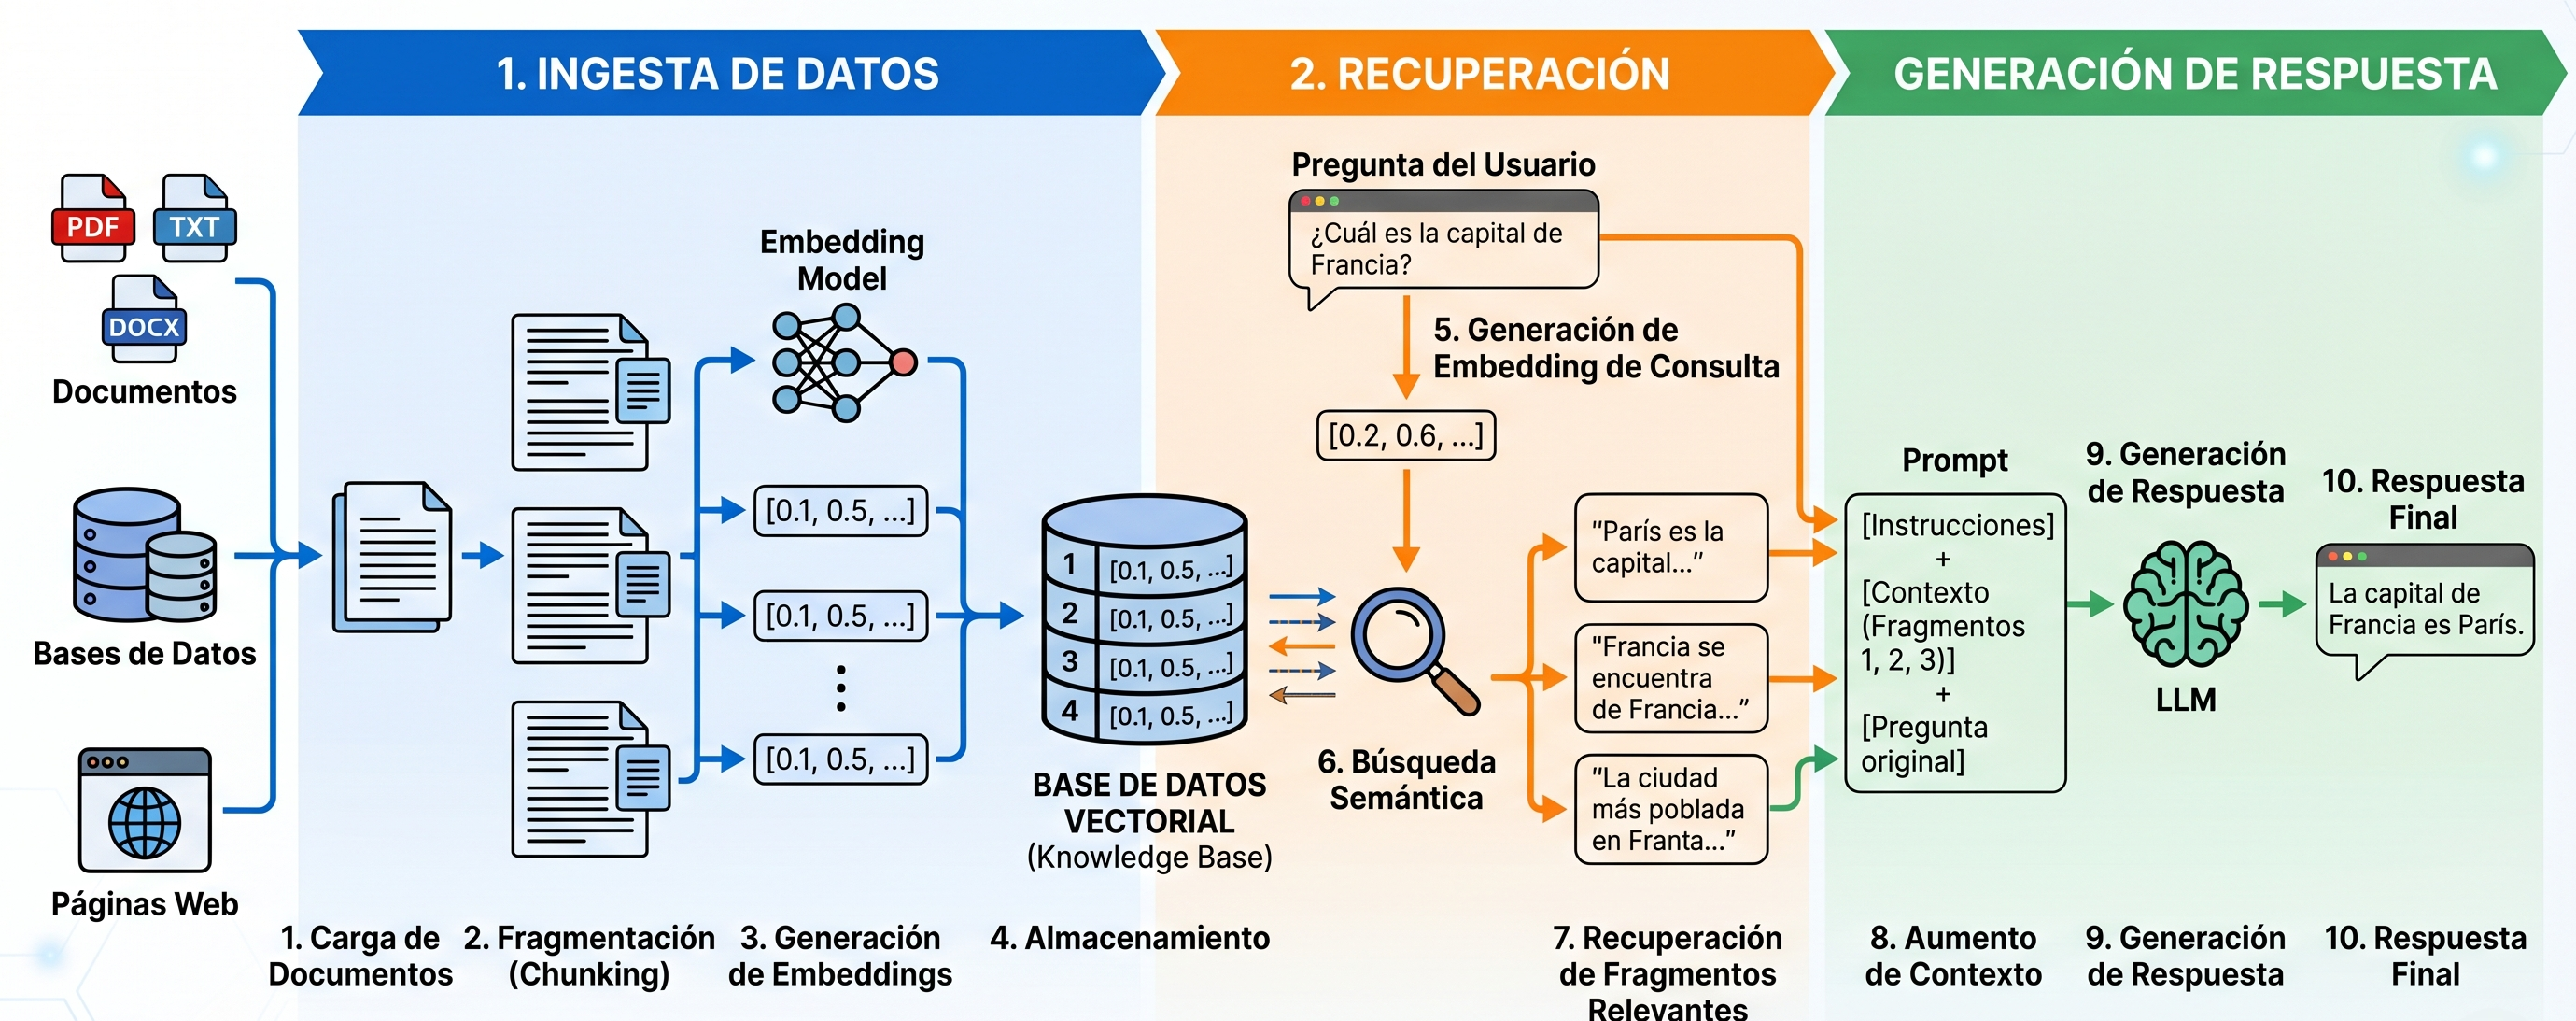
\includegraphics[width=0.8\textwidth]{flujo_rag.png}
    \caption{Estructura típica de un sistema RAG}
    \label{fig:rag_structure}
\end{figure}

\subsection{Embeddings y bases de datos vectoriales}

Un \textit{embedding} es una representación numérica densa de un fragmento de texto en un espacio vectorial de alta dimensionalidad. Dos textos semánticamente similares producirán vectores cercanos en este espacio, lo que permite realizar búsquedas por similitud semántica en lugar de por coincidencia exacta de palabras.

Los modelos de embeddings multilingües son capaces de generar representaciones que capturan el significado del texto independientemente del idioma, lo que resulta esencial para un sistema que opera sobre documentación en español.

Las bases de datos vectoriales, como Pinecone, están optimizadas para almacenar y buscar eficientemente entre millones de vectores. Estas utilizan algoritmos de búsqueda aproximada de vecinos más cercanos (ANN, \textit{Approximate Nearest Neighbors}) que permiten recuperar los documentos más relevantes en milisegundos.

\subsection{Estrategias de fragmentación (chunking)}

La fragmentación o \textit{chunking} es el proceso de dividir documentos extensos en segmentos manejables para su vectorización. La calidad de esta fragmentación impacta directamente en la precisión de la recuperación, y existen diversos tipos como son los siguientes:

\begin{itemize}
    \item \textbf{Fragmentación por tamaño fijo:} Divide el texto en bloques de $n$ caracteres con un solapamiento (\textit{overlap}) configurable. Es simple pero puede romper el contexto de tablas o párrafos.
    \item \textbf{Fragmentación semántica:} Respeta los límites naturales del documento (encabezados, párrafos, tablas) para preservar la coherencia. Herramientas como \texttt{MarkdownTextSplitter} de LangChain utilizan la estructura Markdown como guía para los cortes.
    \item \textbf{Fragmentación asistida por IA:} Herramientas como LlamaParse utilizan modelos de visión para interpretar la estructura del documento, preservando tablas, notas al pie y jerarquías de encabezados.
\end{itemize}

\section{Agentes de Inteligencia Artificial}
\subsection{De LLMs a sistemas agénticos}

Si me paro a pensarlo, un LLM por sí solo funciona como una caja que recibe texto y devuelve texto. Para lo que busco en este proyecto ---un asistente que sea capaz de tomar decisiones, consultar fuentes y mantener el hilo de una conversación--- eso se queda corto. Necesito un paso más: convertir ese modelo en el ``cerebro'' de un agente de IA que, además de generar lenguaje, pueda hacer lo siguiente:

\begin{itemize}
    \item \textbf{Razonar:} Analizar la consulta del usuario y decidir las acciones que debe tomar.
    \item \textbf{Planificar:} Descomponer tareas complejas en subtareas para poder resolverlas de manera más eficiente.
    \item \textbf{Actuar:} Invocar herramientas externas, mediante las que enriquecer la calidad de la información a la que el modelo puede acceder (APIs, bases de datos, buscadores, etc).
    \item \textbf{Recordar:} Mantener un estado conversacional a lo largo de múltiples interacciones con el usuario.
\end{itemize}

\subsection{Grafos de estado: LangGraph}

Una vez que decidí trabajar con agentes, me hacía falta una herramienta que me permitiera orquestar todo esto desde Python. Después de evaluar varias alternativas, opté por utilizar LangGraph, una extensión de LangChain que modela el flujo de un agente como un grafo dirigido de estados. Cada operación se representa como un nodo del grafo, y las transiciones condicionales entre operaciones se definen como aristas.
Este planteamiento ofrece varias ventajas claras frente al esquema clásico de entrada/salida:

\begin{itemize}
    \item \textbf{Flujos condicionales:} En función de la entrada del usuario, el agente podrá tomar caminos diferentes teniendo a su disposición diversas herramientas.
    \item \textbf{Ciclos controlados:} Permite implementar bucles controlados de interacción con el usuario en los cuales el agente pueda solicitar información adicional en caso de ser algo ambigua la consulta.
    \item \textbf{Estado compartido:} Todos los nodos acceden y modifican a un estado global tipado (\texttt{StateSchema}), garantizando la coherencia.
    \item \textbf{Depuración:} Debido a la estructura de grafo facilita la trazabilidad de las decisiones del agente, facilitando de esta manera la identificación de errores.
\end{itemize}

\section{Chatbots institucionales: antecedentes}

La idea de poner un chatbot en una universidad no es nada nueva. Desde hace años, muchas instituciones han desplegado asistentes virtuales apoyándose en motores de Reconocimiento del Lenguaje Natural (NLU) y clasificación de intenciones, con plataformas conocidas como DialogFlow o Rasa. Estas herramientas funcionan razonablemente bien cuando el flujo de diálogo está bien acotado, pero se quedan cortas en cuanto el volumen de información crece. El motivo es que se basan en árboles de decisión y reglas predefinidas, lo que obliga a un mantenimiento constante: cada vez que surge una nueva casuística hay que añadir frases de entrenamiento y mapear la interacción manualmente.

Lo que diferencia a este trabajo de esos enfoques clásicos es el salto de un modelo basado en intenciones a uno generativo y dinámico. Combinando la flexibilidad de los LLMs con el conocimiento institucional actualizado mediante RAG y una estructura agéntica con distintos nodos especializados, el sistema es capaz de localizar la respuesta en la documentación oficial y presentarla de forma clara, sin necesidad de haber previsto cada posible pregunta de antemano.

\section{Tecnologías clave del ecosistema}

\subsection{Lenguaje y Frameworks base}

Como lenguaje principal utilicé Python. Tomé esta decisión de manera muy natural, dado que a día de hoy se considera que es el estándar en todo lo que rodea a la Inteligencia Artificial. Su ecosistema de bibliotecas es enorme y ofrece compatibilidad directa con las herramientas de orquestación que veré a continuación (LangChain, LangGraph), además de con prácticamente cualquier librería de procesamiento de datos que necesite.

Sobre esta base, estructuré el sistema utilizando dos \textit{frameworks} principales, cada uno orientado a una de las capas de la aplicación (frontend/backend):
\begin{itemize}
    \item \textbf{FastAPI (Backend):} para la implementación de la lógica del servidor y la exposición de servicios mediante una API REST y streaming por Server-Sent Events (SSE). Esta tecnología destaca por su alto rendimiento y su soporte nativo ante operaciones asíncronas, característica crítica para gestionar de manera eficiente las llamadas a los modelos de lenguaje y a la base de datos vectorial sin bloquear el hilo principal.
    \item \textbf{Next.js y TypeScript (Frontend):} para la interfaz de usuario. Aunque inicialmente me planteé usar Streamlit por su rapidez de prototipado, pronto requerí un nivel superior de interactividad, modularidad y control estético. La transición a una aplicación desarrollada en Next.js (basado en React) con TypeScript y TailwindCSS me permitió separar limpiamente el cliente del servidor, implementar controles avanzados de sesión por cookies JWT, mostrar estados intermedios del agente a través de eventos en tiempo real, e integrar un panel de feedback y auditoría interactivo sin recargas invasivas de página.
\end{itemize}

\subsection{Orquestación y Lógica Agéntica}

LangChain \cite{langchain_docs} es un framework de código abierto que proporciona abstracciones para conectar LLMs con fuentes de datos externas, cadenas de procesamiento y herramientas. LangGraph \cite{langgraph_docs} extiende este framework con la capacidad de definir grafos de estado, permitiendo flujos de control complejos con nodos y aristas condicionales.

\subsection{Pinecone como base de datos vectorial}

Pinecone \cite{pinecone_docs} es un servicio gestionado de base de datos vectorial que ofrece almacenamiento, indexación y búsqueda de vectores de alta dimensionalidad con baja latencia. Su modelo serverless elimina la necesidad de gestionar infraestructura, lo que simplifica el despliegue.

\subsection{Cohere: embeddings y reranking}

Cohere \cite{cohere_docs} proporciona dos servicios fundamentales para este proyecto: un modelo de embeddings multilingüe (\texttt{embed-multilingual-v3.0}) para la vectorización de documentos en español, y un modelo de reranking (\texttt{rerank-v4.0-pro}) que reordena los resultados de la búsqueda vectorial según su relevancia contextual con la consulta.

\subsection{Groq: inferencia de baja latencia}

Groq \cite{groq_docs} es una plataforma de inferencia que utiliza hardware especializado (LPUs, \textit{Language Processing Units}) diseñado específicamente para la ejecución de modelos de lenguaje. Frente a las GPUs tradicionales, los LPUs ofrecen latencias de inferencia significativamente menores, lo que resulta crítico para un asistente conversacional en tiempo real.

\subsection{LlamaParse: procesamiento de documentos}

LlamaParse \cite{llamaparse_docs} es un servicio de procesamiento de documentos que utiliza modelos de visión por computador para extraer contenido de archivos PDF preservando su estructura original. A diferencia de extractores de texto convencionales, LlamaParse es capaz de interpretar tablas complejas, notas al pie y jerarquías de encabezados, convirtiendo el contenido a formato Markdown estructurado.

\subsection{Encriptado de contraseñas}

Para garantizar la seguridad y privacidad de los usuarios, implementé un flujo de \textit{hashing} para las contraseñas utilizando el algoritmo bcrypt. Lo elegí principalmente porque, además de ofrecer un cifrado unidireccional (irrecuperable), incorpora de forma nativa un sistema de \textit{salting}. Este consiste en añadir datos aleatorios a la contraseña antes de cifrarla, lo que permite ajustar el 'coste' computacional del algoritmo. Esto hace que el sistema sea resistente a ataques de fuerza bruta, garantizando que, incluso ante una filtración de la base de datos, los atacantes no puedan obtener las contraseñas reales.

\subsection{Gestión de la base de datos relacional}

Para la persistencia de los datos, me planteé diversas opciones, tales como MySQL, SQLServer o Oracle. Para el objetivo de este proyecto, consideré que la opción más conveniente era PostgreSQL, puesto que no solo ofrece una buena solución, sino que además ya tenía algo de experiencia previa trabajando con la misma. Se trata de un sistema de gestión de base de datos relacional que se caracteriza por:
\begin{itemize}
    \item \textbf{Integridad y fiabilidad de datos:} garantiza el cumplimiento estricto de las propiedades ACID (Atomicidad, Consistencia, Aislamiento, Durabilidad), lo que le permite ser muy tolerante a fallos, garantizando así transacciones muy seguras.
    \item \textbf{Código abierto y gratuito:} a diferencia de las bases de datos que requieren de una licencia comercial para poder hacer uso de todas sus funciones, esta tecnología al ser \textit{open source} no tiene ningun tipo de coste, conviertiéndola en una alternativa rentable frente a opciones privativas.
    \item \textbf{Rendimiento y escalabilidad:} está diseñado para manejar grandes volúmenes de datos y cargas de trabajo pesadas, lo que le permite ser altamente escalable y eficiente en consultas complejas.
\end{itemize}

Para poder interactuar con la base de datos desde el backend, aunque valoré el uso de \textit{psycopg2}, la cual ofrece una gran velocidad a la hora de resolver tareas sencillas, requería de un ORM (Object-Relational Mapping) más robusto. Finalmente, me decidí por \textit{SQLAlchemy} dado que ofrece tanto el propio ORM como un \textit{SQL Expression Language}, facilitando enormemente la realización de consultas. Además, destaca por su facilidad para gestionar conexiones, migraciones y proteger el sistema frente a vulnerabilidades como la inyección SQL.

\subsection{Arquitectura de despliegue}

Para poner el sistema a disposición de los usuarios finales en un entorno de producción real, opté por una arquitectura de despliegue basada en la contenedorización y en servicios de plataforma en la nube (\textit{Platform as a Service} o PaaS). El objetivo principal de este planteamiento es simplificar la puesta en marcha, asegurar la escalabilidad del sistema y garantizar que la aplicación funcione en producción de la misma forma exacta en que lo hace en el entorno de desarrollo local.

Las dos tecnologías clave que hacen esto posible son \textbf{Docker} y \textbf{Render}:

\begin{itemize}
    \item \textbf{Docker para la contenedorización:} En lugar de lidiar con las diferencias de configuración y dependencias entre servidores, cada componente del sistema (el \textit{frontend} en Next.js (React) y el \textit{backend} en FastAPI) se empaqueta en su propio contenedor Docker utilizando imágenes base estables (como \texttt{node:18-alpine} para el cliente frontend y \texttt{python:3.11-slim-bookworm} para el servidor API backend). Esto encapsula todo lo necesario para la ejecución, aislando las aplicaciones y eliminando por completo el clásico problema del ``en mi máquina funcionaba''.
    
    \item \textbf{Render para la infraestructura en la nube:} Render es una plataforma en la nube que destaca por su facilidad de uso e integración continua con GitHub. Permite desplegar aplicaciones web a partir de un \texttt{Dockerfile} de forma automatizada: cada vez que se sube un cambio al repositorio de producción, Render descarga el código, construye la imagen de Docker y despliega la nueva versión sin tiempo de caída.
\end{itemize}

En el entorno de producción, la arquitectura del sistema se distribuye de manera modular en tres servicios independientes dentro de la nube de Render:

\begin{enumerate}
    \item \textbf{Servicio de Backend (FastAPI):} Configurado como un \textit{Web Service} que expone los endpoints de la API. Se construye utilizando el archivo \texttt{Dockerfile} de la carpeta \texttt{/backend} y gestiona toda la lógica del agente LangGraph.
    
    \item \textbf{Servicio de Frontend (Next.js):} Configurado como otro \textit{Web Service} público. Se compila a partir del \texttt{Dockerfile} de la carpeta \texttt{/frontend} y sirve la interfaz de usuario que consume la API del backend.
    
    \item \textbf{Base de Datos Gestionada (PostgreSQL):} En lugar de ejecutar PostgreSQL dentro de un contenedor autogestionado en producción, se utiliza un servicio de base de datos gestionada provisto directamente por Render. Esto garantiza copias de seguridad automáticas, alta disponibilidad y un rendimiento óptimo sin añadir complejidad de administración.
\end{enumerate}

Para conseguir que todos estos servicios funcionen de manera óptima, la configuración de la aplicación se gestiona enteramente mediante \textbf{variables de entorno}. Siguiendo las buenas prácticas del desarrollo de software moderno (\textit{Twelve-Factor App}), no se almacena ningún tipo de credencial o clave secreta en el código fuente ni dentro de las imágenes Docker. 

En su lugar, Render permite inyectar estas variables en tiempo de ejecución de manera segura a través de su panel de administración. De esta forma, el \textit{backend} recibe las claves de acceso de los proveedores de servicios (\texttt{GROQ\_API\_KEY}, \texttt{COHERE\_API\_KEY}, \texttt{PINECONE\_API\_KEY} y \texttt{LLAMA\_CLOUD\_API\_KEY}), la clave secreta de firmado (\texttt{SECRET\_KEY}) y la dirección de conexión a la base de datos (\texttt{DATABASE\_URL}). Por su parte, el \textit{frontend} únicamente necesita conocer la URL pública de la API del backend (\texttt{API\_URL}) para poder enviarle las peticiones de los usuarios. Esta separación no solo protege la seguridad de nuestras credenciales, sino que dota al sistema de una enorme flexibilidad para cambiar de entorno o actualizar \textit{API keys} sin necesidad de recompilar una sola línea de código.
% ============================================================
% PARTE II: METODOLOGÍA Y PLANIFICACIÓN
% ============================================================
\part{Metodología y Planificación}

\chapter{Metodología de desarrollo}
\section{Ciclo de vida del proyecto}

Desde el primer momento tuve claro que un enfoque en cascada no iba a funcionar para este proyecto. Al tratarse de un sistema donde las decisiones sobre modelos, estrategias de fragmentación o hiperparámetros dependen en gran medida de resultados empíricos ---es decir, de probar y ver qué sale---, necesitaba un ciclo de vida que me permitiera equivocarme pronto y corregir rápido. Por eso se optó por un enfoque iterativo e incremental, en el que cada iteración produce un incremento funcional del sistema.

En la práctica, cada iteración ha seguido el ciclo: análisis $\rightarrow$ diseño $\rightarrow$ implementación $\rightarrow$ pruebas $\rightarrow$ retroalimentación. Esto me permitió ir refinando componentes críticos como el pipeline de ingesta o la configuración de los modelos de lenguaje a medida que aprendía de los errores.

\section{Metodología Scrum adaptada}

Aunque Scrum está pensado para equipos multidisciplinares, sus principios básicos de flexibilidad y entrega incremental encajaban muy bien con el carácter de este proyecto. Lógicamente, no tenía sentido realizar reuniones de sincronización diarias (las tradicionales \textit{dailies}) al ser un único desarrollador. Por ello, decidí adaptar el marco de trabajo a un formato unipersonal, simplificando la gestión de tareas pero manteniendo la disciplina de sprints cortos de dos semanas y el enfoque en desarrollar incrementos de software que se pudieran probar.

La dinámica real consistió en estructurar el trabajo en torno a las tutorías periódicas con mis tutores del TFG. En cada reunión se actuaba de forma similar a una revisión de sprint: evaluábamos el progreso, detectábamos fallos de diseño y decidíamos las prioridades para el siguiente ciclo de desarrollo.

\subsection{Roles del proyecto}

Al tratarse de un TFG individual, los roles tradicionales de Scrum se adaptaron para reflejar la relación real entre el alumno y los directores:
\begin{itemize}
    \item \textbf{Product Owner (Clientes):} Este papel fue asumido por mis tutores del TFG, José Enrique Sánchez López y Pablo Reina Jiménez. Como expertos en el dominio y directores del trabajo, se encargaban de priorizar qué funcionalidades eran prioritarias para el asistente, proponer la documentación de la US a ingestar y validar que las respuestas generadas por el agente conversacional fueran rigurosas y útiles.
    \item \textbf{Scrum Master y Equipo de Desarrollo:} Yo mismo asumí estas funciones. Como desarrollador, me encargaba de codificar el frontend, el backend y configurar el pipeline RAG. Como Scrum Master, mi labor consistía en autoorganizar el trabajo, mantener al día el backlog y buscar soluciones rápidas a los bloqueos técnicos que surgían durante las pruebas locales.
\end{itemize}

\subsection{Artefactos utilizados}

Para llevar un control real del progreso sin sobrecargar el desarrollo con burocracia innecesaria, utilicé tres artefactos adaptados:
\begin{itemize}
    \item \textbf{Backlog del Producto:} Una lista dinámica con las funcionalidades y mejoras que queríamos para el asistente. Esta lista varió enormemente a lo largo del proyecto a medida que nos topábamos con limitaciones de hardware o problemas de precisión en las respuestas del modelo.
    \item \textbf{Backlog del Sprint:} Las tareas concretas seleccionadas para realizarse entre tutorías (por ejemplo, implementar la comunicación entre backend y base de datos relacional, o pulir la visualización del chat).
    \item \textbf{Incremento:} La versión ejecutable y probada del software al final de cada ciclo. El objetivo fue que el asistente tuviera siempre una base estable y funcional sobre la que añadir la siguiente mejora.
\end{itemize}

\subsection{Dinámica de trabajo y reuniones}

Las ceremonias clásicas de Scrum se simplificaron para adaptarse al contexto académico de tutorías:
\begin{itemize}
    \item \textbf{Planificación del Sprint:} Al comienzo de cada ciclo de dos semanas, definía los objetivos técnicos concretos a desarrollar en base a las recomendaciones e ideas surgidas en la tutoría previa.
    \item \textbf{Revisión y Retrospectiva:} En cada reunión con los tutores presentaba el incremento de software y probábamos juntos el comportamiento del agente. Esto nos servía para identificar qué partes (como la extracción de tablas de los PDFs o el diseño de los nodos en LangGraph) no estaban funcionando bien y debían replantearse de cara al siguiente sprint.
\end{itemize}

\section{Herramientas de gestión y desarrollo}

Para dar soporte a esta metodología de trabajo y asegurar la reproducibilidad del entorno de desarrollo, utilicé las siguientes herramientas:
\begin{itemize}
    \item \textbf{Control de versiones:} Git como herramienta local y GitHub como repositorio remoto, lo que me permitió mantener un historial ordenado de cambios y proteger el código de pérdidas accidentales.
    \item \textbf{Gestión de tareas:} En lugar de usar herramientas corporativas complejas, organicé el backlog a través de listas de tareas priorizadas y notas vinculadas directamente con las actas de reuniones de tutoría.
    \item \textbf{Entorno de desarrollo:} Visual Studio Code, configurado con extensiones específicas para Python (depuración y tipado), Docker (para el control de los contenedores locales) y LaTeX (para la redacción de la memoria).
    \item \textbf{Entorno de ejecución local:} Docker y Docker Compose, esenciales para levantar de manera consistente y en pocos segundos el backend, frontend y la base de datos PostgreSQL, asegurando la reproducibilidad del entorno en cualquier máquina.
\end{itemize}

\chapter{Planificación y desviaciones}
\section{Definición estimada de sprints}

Para estructurar las 20 semanas de duración estimadas para el desarrollo del TFG, se organizó el cronograma de trabajo en 10 sprints de dos semanas cada uno. La siguiente tabla describe los hitos principales que se plantearon en cada uno de estos bloques temporales:

\begin{table}[H]
    \centering
    \caption{Planificación inicial estimada de sprints del proyecto}
    \begin{tabular}{@{}clp{8cm}@{}}
        \toprule
        \textbf{Sprint} & \textbf{Periodo} & \textbf{Hito principal objetivo}                                      \\
        \midrule
        1               & Semanas 1--2     & Investigación del estado del arte, selección de APIs y requisitos.    \\
        2               & Semanas 3--4     & Pipeline de ingesta: extracción semántica de PDFs oficiales.          \\
        3               & Semanas 5--6     & Conexión del RAG básico: embeddings de Cohere y Pinecone.             \\
        4               & Semanas 7--8     & Diseño lógico y programación del grafo de estados en LangGraph.       \\
        5               & Semanas 9--10    & Desarrollo del backend FastAPI y diseño del modelo de datos.         \\
        6               & Semanas 11--12   & Creación de la interfaz modular de chat en Next.js(React).                     \\
        7               & Semanas 13--14   & Migración a la API de Groq para la optimización de latencias.        \\
        8               & Semanas 15--16   & Contenedorización de todos los servicios locales con Docker Compose.  \\
        9               & Semanas 17--18   & Batería de pruebas de validación y evaluación cuantitativa.           \\
        10              & Semanas 19--20   & Redacción final de la memoria y preparación de la defensa.            \\
        \bottomrule
    \end{tabular}
\end{table}

\section{Diagrama de Gantt}

Para visualizar mejor la distribución temporal de las tareas y comprender el solapamiento de las fases de desarrollo con la documentación y las pruebas, elaboré un diagrama de Gantt. 

Este diagrama (representado en la Figura~\ref{fig:gantt}) actúa como una estimación del cronograma lógico seguido. Aunque en el día a día el desarrollo real fue dinámico e interactivo debido al ensayo y error, el Gantt sirve como marco de referencia para entender los plazos teóricos del proyecto.

\begin{figure}[H]
    \centering
    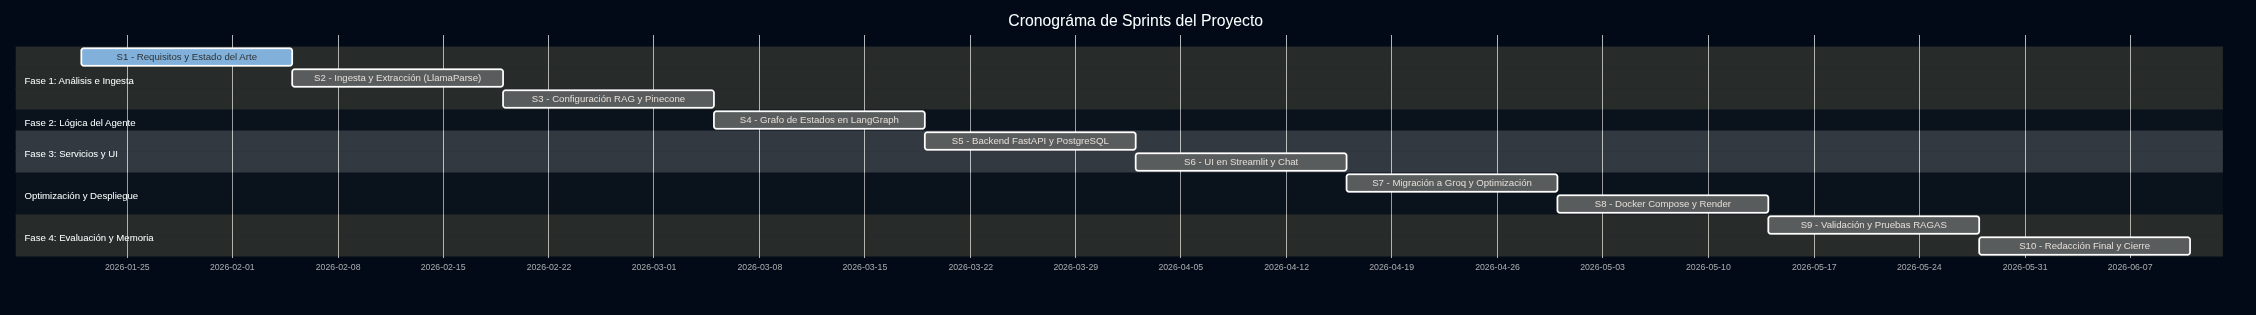
\includegraphics[width=1\textwidth]{diagrama_gantt.png}
    \caption{Diagrama de Gantt de la planificación estimada del TFG}
    \label{fig:gantt}
\end{figure}

\section{Estimación de esfuerzo}

Se planificó una dedicación media de entre 15 y 20 horas semanales durante las 20 semanas del proyecto, estimando un total acumulado de unas 350 horas de trabajo real. La distribución del tiempo según las distintas actividades del proyecto se desglosó de la siguiente forma aproximada:

\begin{itemize}
    \item \textbf{Investigación teórica y estado del arte:} 15\% del tiempo (lectura de artículos sobre RAG, agentes conversacionales y documentación de APIs).
    \item \textbf{Desarrollo del pipeline RAG e ingesta:} 25\% del tiempo (pruebas de extracción de PDFs, vectorización y almacenamiento).
    \item \textbf{Orquestación del agente inteligente (LangGraph):} 20\% del tiempo (definición de nodos, transiciones condicionales y prompts de enrutamiento).
    \item \textbf{Backend y Frontend:} 15\% del tiempo (creación de la API de FastAPI, base de datos relacional e interfaz modular de chat en Next.js (React) con TypeScript).
    \item \textbf{Evaluación y validación:} 10\% del tiempo (baterías de pruebas para evaluar la fiabilidad de las respuestas).
    \item \textbf{Redacción de la memoria y documentación:} 15\% del tiempo (documentación técnica y redacción de este documento).
\end{itemize}

\section{Análisis de riesgos}

Para evitar que el desarrollo se estancara por problemas técnicos imprevistos, realicé un análisis de riesgos inicial evaluando su probabilidad e impacto y definiendo medidas paliativas concretas:

\begin{table}[H]
    \centering
    \caption{Matriz de riesgos del proyecto y sus estrategias de mitigación}
    \begin{tabular}{@{}p{4.5cm}ccp{5.5cm}@{}}
        \toprule
        \textbf{Riesgo identificado}                          & \textbf{Prob.} & \textbf{Imp.} & \textbf{Estrategia de mitigación planteada}                     \\
        \midrule
        Límites de cuota gratuitos en APIs (Groq, LlamaParse)  & Alta           & Alto          & Diseñar un sistema multi-modelo usando LLMs ligeros.            \\
        Alucinaciones e invenciones en respuestas del agente   & Media          & Alto          & Forzar temperatura baja (0.1) y RAG estricto con fuentes.       \\
        Pérdida de estructura en tablas complejas de los PDFs  & Alta           & Medio         & Migración a LlamaParse con prompts específicos de extracción.   \\
        Latencias excesivas de inferencia en tiempo de chat    & Media          & Medio         & Uso de hardware optimizado (LPUs de Groq) para inferencia rápida.\\
        Pérdida de contexto en chats muy prolongados           & Baja           & Bajo          & Implementación de memoria de ventana y compresión por resúmenes. \\
        Curva de aprendizaje del framework LangGraph           & Media          & Medio         & Reservar margen de tiempo en los primeros sprints de diseño.    \\
        \bottomrule
    \end{tabular}
    \label{tab:riesgos}
\end{table}

\section{Desviaciones sobre la planificación inicial}

En un proyecto centrado en la integración de Inteligencia Artificial y modelos de lenguaje, la teoría rara vez coincide al 100\% con la práctica. La naturaleza exploratoria del desarrollo hizo que el cronograma real sufriera variaciones significativas respecto a la planificación estimada en el Gantt, destacando cuatro desviaciones principales:

\begin{itemize}
    \item \textbf{Cambio en la infraestructura de inferencia (Sprints 4 y 7):} Inicialmente, la intención era que todo el sistema funcionara en local utilizando modelos de código abierto (como Llama 3.1 8B) a través de Ollama. Sin embargo, al probar las primeras ejecuciones del agente LangGraph, los tiempos de respuesta superaban con creces el minuto por consulta debido a la falta de potencia de hardware local. Esto obligó a cambiar el rumbo técnico a mitad del proyecto para migrar todas las llamadas de inferencia a la API en la nube de Groq.
    
    \item \textbf{Reestructuración del pipeline de ingesta (Sprints 2 y 3):} La fragmentación estándar de los documentos oficiales (normativas de matrícula o guías de viaje) rompía por completo las tablas y los anexos, lo que provocaba que el asistente diera respuestas erróneas sobre plazos y cuantías de dinero. Tuve que detener el plan de desarrollo previsto para investigar tecnologías de extracción avanzada, migrando primero a Docling y finalmente a LlamaParse. El proceso de solucionar el problema del "doble splitter" (donde un formateador secundario rompía de nuevo las tablas de LlamaParse) consumió casi dos semanas completas que no estaban contempladas originalmente.
    
    \item \textbf{Gestión de cuotas y depuración de la memoria:} El testing del agente consumió rápidamente los límites de tokens diarios de las capas gratuitas de las APIs. Esto provocó parones forzados en el desarrollo y obligó a implementar a toda prisa la funcionalidad de compresión y resumen de memoria histórica mediante tareas en segundo plano en FastAPI, con el fin de ahorrar tokens en cada turno de chat.
    
    \item \textbf{Reconstrucción de la interfaz frontend (Sprints 5 y 6):} Inicialmente se contempló el uso de Streamlit para el desarrollo rápido del frontend. No obstante, al avanzar en los requisitos de interactividad, control estético personalizado y la necesidad de gestionar sesiones de usuario mediante cookies JWT, flujos Server-Sent Events (SSE) interactivos y un panel de administración avanzado, Streamlit demostró limitaciones de modularidad y escalabilidad. Esto forzó a pivotar la arquitectura del cliente hacia Next.js (React) con TypeScript. Reconstruir la interfaz desde cero supuso un esfuerzo extra de desarrollo y una curva de aprendizaje no prevista que desplazó ligeramente el calendario de integración.
\end{itemize}

\section{Estimación de costes}

Aunque este proyecto es puramente académico, resulta interesante hacer el ejercicio de estimar cuánto costaría si se tratase de un encargo profesional real desarrollado por un ingeniero de software junior. He dividido la estimación en tres partidas: personal, recursos materiales y costes indirectos.

\subsection{Costes de personal}
Tomando como referencia la estimación de 350 horas de dedicación calculada en la sección anterior, y asumiendo un coste por hora estándar para un perfil de desarrollador junior de 15 €/hora, el coste de personal asciende a:
\begin{itemize}
    \item \textbf{Desarrollador Junior:} 350 horas $\times$ 15 €/hora = 5.250 €
\end{itemize}

\subsection{Costes de hardware y software}
\begin{itemize}
    \item \textbf{Hardware:} Empleé un equipo informático portátil valorado en 1.200 €. Considerando un periodo de amortización de 4 años, y dado que el proyecto duró 5 meses, la cuota de amortización imputable al proyecto es de aproximadamente 125 €.
    \item \textbf{Software y APIs:} El desarrollo lo apoyé mayoritariamente en herramientas de código abierto (Python, Next.js (React), FastAPI, Docker). Los servicios de IA y bases de datos vectoriales (Groq, Cohere, Pinecone, LlamaParse) los utilicé en su capa gratuita (\textit{Free Tier'}), por lo que el coste directo en este apartado es de 0 €. Sin embargo, en un entorno de producción, los costes de inferencia y almacenamiento escalarían según el uso.
\end{itemize}

\subsection{Costes indirectos}
Se contemplan gastos de suministros como electricidad y conexión a internet durante los 5 meses de desarrollo, que se estiman conservadoramente en 20 € mensuales imputables al proyecto.
\begin{itemize}
    \item \textbf{Suministros:} 5 meses $\times$ 20 €/mes = 100 €
\end{itemize}

\subsection{Coste total del proyecto}
Sumando todas las partidas anteriores, obtengo el coste total estimado del proyecto:

\begin{table}[H]
    \centering
    \caption{Presupuesto total estimado}
    \begin{tabular}{@{}lr@{}}
        \toprule
        \textbf{Concepto}                 & \textbf{Coste estimado (€)} \\
        \midrule
        Costes de Personal                & 5.250,00                    \\
        Costes de Hardware (Amortización) & 125,00                      \\
        Costes de Software y APIs         & 0,00                        \\
        Costes Indirectos                 & 100,00                      \\
        \midrule
        \textbf{Base Imponible}           & \textbf{5.475,00}           \\
        IVA (21\%)                        & 1.1149,75                    \\
        \midrule
        \textbf{Total Presupuesto}        & \textbf{6.624,75}           \\
        \bottomrule
    \end{tabular}
    \label{tab:presupuesto}
\end{table}

% ============================================================
% PARTE III: ANÁLISIS Y DISEÑO
% ============================================================
\part{Análisis y Diseño}
\chapter{Análisis de requisitos}
\section{Requisitos funcionales}

\begin{longtable}{@{}cp{12cm}@{}}
    \caption{Requisitos funcionales del sistema}                                                                                   \\
    \toprule
    \textbf{ID} & \textbf{Descripción}                                                                                             \\
    \midrule
    \endfirsthead

    \caption[]{Requisitos funcionales del sistema (continuación)}                                                                  \\
    \toprule
    \textbf{ID} & \textbf{Descripción}                                                                                             \\
    \midrule
    \endhead

    RF-01       & El sistema debe permitir el registro de usuarios mediante email y contraseña.                                    \\
    RF-02       & El sistema debe permitir la autenticación de usuarios mediante JWT.                                              \\
    RF-03       & El usuario debe poder crear, renombrar y eliminar conversaciones.                                                \\
    RF-04       & El sistema debe procesar la consulta del usuario y generar una respuesta fundamentada en documentos oficiales.   \\
    RF-05       & El sistema debe clasificar la intención del usuario y enrutar la consulta al nodo especializado correspondiente. \\
    RF-06       & El sistema debe rechazar amablemente consultas que no estén relacionadas con trámites de la US.                  \\
    RF-07       & El sistema debe solicitar aclaraciones al usuario cuando la consulta sea ambigua.                                \\
    RF-08       & El sistema debe mostrar las fuentes y referencias consultadas junto con cada respuesta.                          \\
    RF-09       & El sistema debe mantener el contexto de la conversación a lo largo de múltiples turnos.                          \\
    RF-10       & Los administradores deben poder ingestar nuevos documentos PDF al sistema desde la interfaz.                     \\
    RF-11       & El sistema debe generar automáticamente títulos descriptivos para las conversaciones.                            \\
    RF-12       & El sistema debe comprimir la memoria de conversaciones largas para mantener la coherencia.                       \\
    RF-13       & El sistema debe mostrar a los administradores las cuentas de usuario existentes en el programa.                  \\
    RF-14       & El sistema debe permitir a los administradores eliminar cuentas de usuario.                                      \\
    RF-15       & El sistema debe permitir a los administradores convertir a otros usuarios en administradores.                    \\
    RF-16       & El sistema debe permitir a los administradores degradar a otros administradores en usuarios.                     \\
    \bottomrule
\end{longtable}

\section{Requisitos no funcionales}

\begin{table}[H]
    \centering
    \caption{Requisitos no funcionales del sistema}
    \begin{tabular}{@{}cp{12cm}@{}}
        \toprule
        \textbf{ID} & \textbf{Descripción}                                                                                     \\
        \midrule
        RNF-01      & El tiempo de respuesta del agente no debe superar los 20 segundos.                                       \\
        RNF-02      & El sistema debe desplegarse mediante contenedores Docker para garantizar la portabilidad.                \\
        RNF-03      & Las contraseñas deben almacenarse hasheadas con bcrypt.                                                  \\
        RNF-04      & La interfaz debe ser accesible desde cualquier navegador web moderno.                                    \\
        RNF-05      & El sistema debe ser capaz de procesar documentos PDF de hasta 100 páginas.                               \\
        RNF-06      & Las respuestas del agente deben basarse exclusivamente en los documentos ingestados (sin alucinaciones). \\
        RNF-07      & La arquitectura debe permitir la adición de nuevos tipos de nodos sin modificar el núcleo del sistema.   \\
        \bottomrule
    \end{tabular}
\end{table}

\section{Casos de uso}

Los principales casos de uso identificados son:

\begin{itemize}
    \item \textbf{CU-01: Registrarse.} Un usuario nuevo crea una cuenta proporcionando email y contraseña.
    \item \textbf{CU-02: Iniciar sesión.} Un usuario registrado se autentica para acceder al sistema.
    \item \textbf{CU-03: Realizar consulta burocrática.} El usuario formula una pregunta sobre normativa o trámites de la US y recibe una respuesta fundamentada.
    \item \textbf{CU-04: Gestionar conversaciones.} El usuario crea, renombra o elimina sus conversaciones.
    \item \textbf{CU-05: Ingestar documento (Admin).} Un administrador sube un nuevo PDF para ampliar la base de conocimiento del agente.
    \item \textbf{CU-06: Gestionar usuarios (Admin).} Un administrador puede gestionar usuarios ya sea añadiendo como nuevo administrador, eliminándolo, degradándolo a usuario normal.
\end{itemize}

\chapter{Diseño de la arquitectura}
\section{Arquitectura general del sistema}

El sistema sigue una arquitectura de microservicios contenedorizados orquestados mediante Docker Compose. Los tres servicios principales son:

\begin{itemize}
    \item \textbf{Frontend (Next.js + TypeScript):} Interfaz web que se comunica con el backend vía HTTP REST y Server-Sent Events (SSE). Puerto 8501.
    \item \textbf{Backend (FastAPI):} API REST que gestiona la autenticación, las conversaciones y orquesta el agente LangGraph. Puerto 8000.
    \item \textbf{Base de datos (PostgreSQL 15):} Almacena usuarios, conversaciones y mensajes. Puerto 5432.
\end{itemize}

Adicionalmente, el sistema se conecta con servicios externos en la nube:
\begin{itemize}
    \item \textbf{Pinecone:} Base de datos vectorial para almacenamiento y búsqueda de embeddings.
    \item \textbf{Groq:} API de inferencia para los modelos Llama 3.1 8B y Llama 3.3 70B.
    \item \textbf{Cohere:} API para generación de embeddings y reranking de documentos.
    \item \textbf{LlamaParse:} API para el procesamiento inteligente de PDFs.
\end{itemize}

\section{Arquitectura del backend (FastAPI)}
\subsection{Modelo de datos}

El modelo relacional del sistema se compone de tres entidades principales implementadas con SQLAlchemy ORM:

\begin{itemize}
    \item \textbf{Usuario:} Almacena el email, contraseña hasheada, rol de administrador y fecha de creación. Relación uno a muchos con Conversación.
    \item \textbf{Conversación:} Contiene el título (auto-generado), un campo de resumen de memoria para conversaciones largas y la referencia al usuario propietario. Relación uno a muchos con Mensaje.
    \item \textbf{Mensaje:} Almacena el rol (user/assistant), el contenido textual, las referencias a documentos consultados (en formato JSON) y la marca temporal.
\end{itemize}

Las relaciones incluyen eliminación en cascada: al eliminar un usuario se eliminan sus conversaciones, y al eliminar una conversación se eliminan sus mensajes.

\begin{figure}[H]
    \centering
    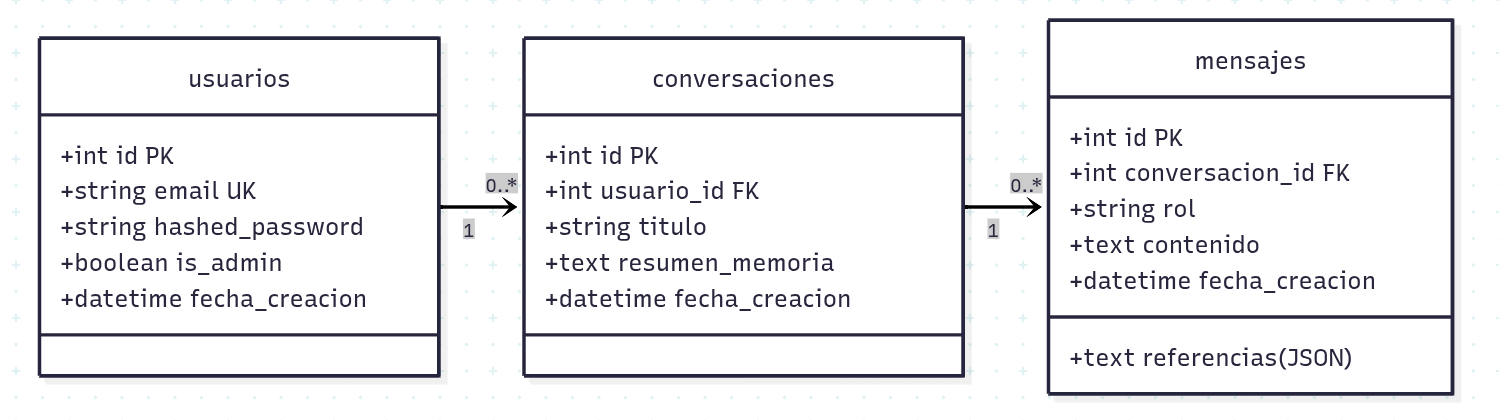
\includegraphics[width=1\textwidth]{modelo_de_datos.png}
    \caption{Modelo de datos del sistema}
    \label{fig:modelo_datos}
\end{figure}

\subsection{Endpoints de la API REST}

\begin{table}[H]
    \centering
    \caption{Endpoints principales de la API}
    \begin{tabular}{@{}lp{5.3cm}p{7.5cm}@{}}
        \toprule
        \textbf{Método} & \textbf{Ruta}                                   & \textbf{Descripción}                          \\
        \midrule
        POST            & \texttt{/auth/registro}                          & Registro de nuevo usuario                     \\
        POST            & \texttt{/auth/login}                             & Autenticación con email/contraseña            \\
        GET             & \texttt{/auth/me}                                & Datos del usuario autenticado                 \\
        GET             & \texttt{/conversaciones}                         & Lista de conversaciones del usuario           \\
        POST            & \texttt{/conversaciones}                         & Crear nueva conversación                      \\
        GET             & \texttt{/conversaciones/\allowbreak\{\allowbreak{}id\}/\allowbreak{}mensajes} & Historial de mensajes                         \\
        POST            & \texttt{/conversaciones/\allowbreak\{\allowbreak{}id\}/\allowbreak{}chat}     & Enviar mensaje y obtener respuesta del agente \\
        POST            & \texttt{/conversaciones/\allowbreak\{\allowbreak{}id\}/\allowbreak{}mensajes/\allowbreak\{\allowbreak{}mid\}/\allowbreak{}feedback} & Enviar valoración y comentario         \\
        PUT             & \texttt{/conversaciones/\allowbreak\{\allowbreak{}id\}}                          & Renombrar conversación                        \\
        DELETE          & \texttt{/conversaciones/\allowbreak\{\allowbreak{}id\}}                          & Eliminar conversación                         \\
        GET             & \texttt{/admin/\allowbreak{}feedback/\allowbreak{}negativo}                      & Listar feedback negativo y referencias (Admin)      \\
        POST            & \texttt{/admin/ingestar}                         & Subir e indexar archivo PDF (Admin)           \\
        DELETE          & \texttt{/admin/documentos}                       & Borrar base de datos vectorial (Admin)        \\
        GET             & \texttt{/admin/usuarios}                         & Listar cuentas de usuarios (Admin)            \\
        DELETE          & \texttt{/admin/usuarios/\allowbreak\{\allowbreak{}id\}}                          & Eliminar cuenta de usuario (Admin)            \\
        PUT             & \texttt{/admin/usuarios/\allowbreak\{\allowbreak{}id\}/\allowbreak{}admin}      & Conceder/revocar rol de admin (Admin)         \\
        GET             & \texttt{/documentos}                             & Listar los nombres de los documentos en Pinecone \\
        \bottomrule
    \end{tabular}
\end{table}

\subsection{Políticas de origen cruzado (CORS)}

Dado que el frontend (Next.js) y el backend (FastAPI) corren en puertos o subdominios independientes, los navegadores bloquean de forma nativa las peticiones HTTP cruzadas. Para solucionar esto, configuré el middleware de CORS en FastAPI (\texttt{CORSMiddleware}) para permitir el acceso de forma controlada a los métodos y cabeceras necesarios, garantizando que el chat y el streaming por SSE funcionen correctamente sin bloqueos del navegador.

\subsection{Autenticación, Autorización y Roles}

El sistema implementa un control de accesos basado en tokens JWT (\textit{JSON Web Tokens}) firmado mediante el algoritmo simétrico HS256. Al iniciar sesión, el servidor valida las credenciales y devuelve el token, el cual expira a los 7 días. El cliente envía este token en la cabecera HTTP de autorización para cualquier operación.

A nivel de base de datos, implementé roles diferenciados mediante la columna booleana \texttt{is\_admin} en la tabla de usuarios. Esto habilita dos niveles de permisos:
\begin{itemize}
    \item \textbf{Rol de Usuario:} Permite registrarse, iniciar sesión, crear conversaciones de chat y enviar feedback sobre las respuestas.
    \item \textbf{Rol de Administrador:} Otorga acceso a todos los endpoints bajo la ruta raíz \texttt{/admin}. Esto habilita las funciones críticas de:
    \begin{enumerate}
        \item \textbf{Gestión de Usuarios:} Listar todos los perfiles de usuario de la plataforma, eliminar cuentas y promover o degradar cuentas concediendo el rol de administrador.
        \item \textbf{Gestión de Documentos:} Ingestar nuevos PDFs con las normativas de la US o vaciar la base de datos vectorial de Pinecone mediante la llamada a \texttt{DELETE /admin/documentos}.
        \item \textbf{Auditoría de Feedback:} Inspeccionar las valoraciones negativas recibidas para corregir el RAG.
    \end{enumerate}
\end{itemize}

\subsection{Modularización y Desacoplamiento (Capa CRUD y Servicios)}

A medida que el backend crecía, me di cuenta de que mantener todo el código en un único archivo (\texttt{main.py}) era una mala idea. El archivo principal acumulaba más de 500 líneas y mezclaba demasiadas responsabilidades: la definición de endpoints, la inyección de dependencias de usuario, la lógica de acceso a la base de datos con SQLAlchemy y la orquestación del streaming SSE con LangGraph. Esto no solo dificultaba enormemente la lectura y la depuración del código, sino que ponía en riesgo la escalabilidad del sistema.

Para solucionar este problema de acoplamiento, decidí llevar a cabo una refactorización profunda estructurando el backend en una arquitectura modular por capas:

\begin{itemize}
    \item \textbf{Capa de Controladores (Routers):} Dividí los endpoints de la API REST utilizando \texttt{APIRouter} de FastAPI en archivos independientes dentro de una nueva carpeta \texttt{/routers}: \texttt{auth.py} (para el registro, login y perfil), \texttt{conversaciones.py} (para la gestión de chats y mensajes), \texttt{admin.py} (para operaciones administrativas) y \texttt{documentos.py} (para consultas del RAG).
    \item \textbf{Capa CRUD/Acceso a Datos (\texttt{crud.py}):} Con el fin de aislar las consultas y modificaciones en la base de datos relacional, extraje todas las llamadas directas de SQLAlchemy (\texttt{db.query}, \texttt{db.commit}, etc.) fuera de los controladores. Aunque consideré llamarle a esta capa \textit{Repository} de acuerdo con patrones formales como DDD (Domain-Driven Design), preferí mantener el término \texttt{crud.py} por ser la convención estándar recomendada en la documentación oficial de FastAPI.
    \item \textbf{Capa de Servicios de Negocio (\texttt{services/}):} Endpoints extremadamente complejos como la transmisión asíncrona por Server-Sent Events (SSE) en \texttt{enviar\_mensaje} los simplifiqué abstrayendo sus responsabilidades. Creé un servicio de chat (\texttt{chat\_service.py}) encargado de dar formato al historial reciente e interactuar con el agente en segundo plano, dejando el router del endpoint con apenas 20 líneas de código dedicadas a validar la petición HTTP y retornar la respuesta en streaming.
\end{itemize}

Esta separación de responsabilidades no solo incrementó drásticamente la legibilidad del proyecto, sino que me permitió solventar un bug latente de tipado en el formateador del stream del agente (al extraer claves con un iterador incorrecto en tiempo de ejecución) y facilitó la integración limpia de las dependencias comunes de autorización mediante tipados avanzados con \texttt{Annotated} de Python.

\section{Diseño del agente conversacional}
\subsection{Grafo de estados (LangGraph)}

Implementé el agente como un \texttt{StateGraph} de LangGraph con ocho nodos y transiciones condicionales. El estado compartido entre nodos se define mediante un \texttt{TypedDict} (\texttt{StateSchema}) con los siguientes campos: \texttt{pregunta}, \texttt{pregunta\_reformulada}, \texttt{historial}, \texttt{historial\_formateado}, \texttt{contexto}, \texttt{stream} y \texttt{referencias}.

El flujo general del grafo es:

\begin{enumerate}
    \item \textbf{START $\rightarrow$ Estado Inicial:} Formatea el historial de la conversación.
    \item \textbf{Estado Inicial $\rightarrow$ Recuperador | Rechazo:} Decide si la consulta es relevante para el dominio.
    \item \textbf{Recuperador $\rightarrow$ Entrevistador | Búsqueda Web | Clasificador:} Decide si la información es suficiente (va al clasificador), ambigua (va al entrevistador) o insuficiente (va a la búsqueda web de fallback).
    \item \textbf{Búsqueda Web $\rightarrow$ Clasificador:} Enriquece el contexto con la búsqueda externa y continúa hacia el clasificador.
    \item \textbf{Clasificador $\rightarrow$ Procedimental | Calendario | Normativo | Baremo:} Enruta la consulta al nodo resolutor experto adecuado.
    \item \textbf{Nodos finales $\rightarrow$ END:} Genera la respuesta definitiva y finaliza el flujo.
\end{enumerate}

\begin{figure}[H]
    \centering
    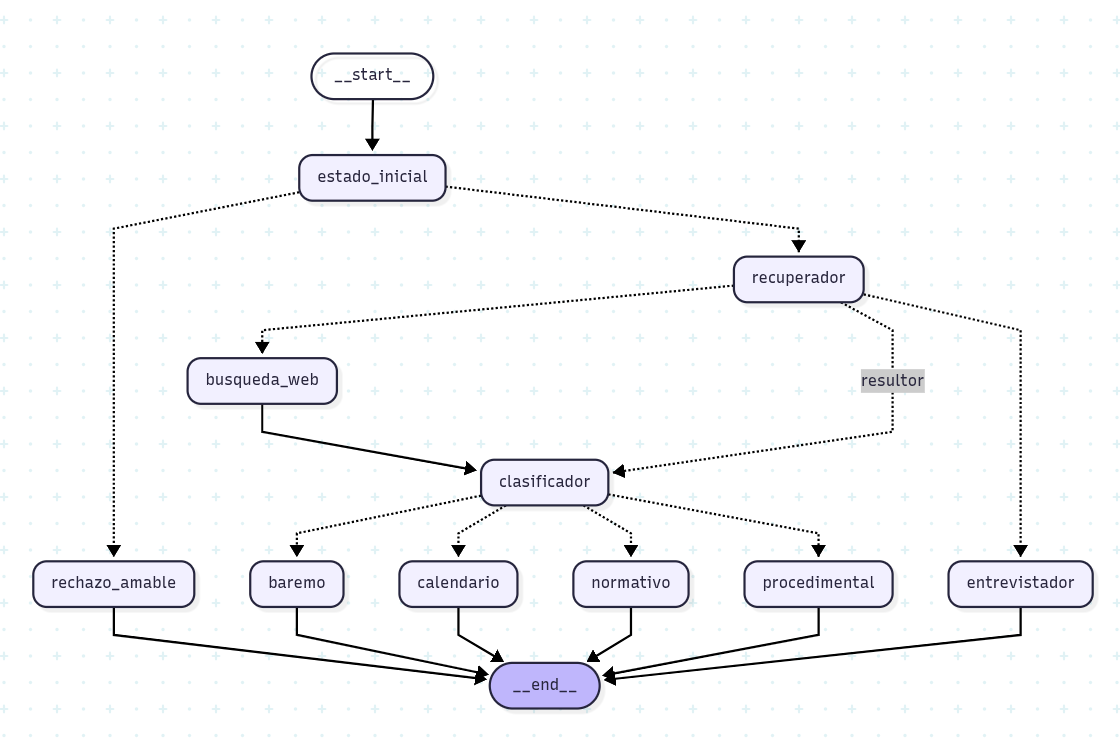
\includegraphics[width=1\textwidth]{diagrama_estados_version_final.png}
    \caption{Versión final diagrama de estados}
    \label{fig:diag_estados_final}
\end{figure}

\subsection{Nodo Estado Inicial}
Formatea el historial de mensajes de la conversación en un formato legible (``rol: contenido'') que será utilizado por los prompts de los nodos posteriores.

\subsection{Nodo Router: clasificación de intenciones}
Utiliza un LLM clasificador ultra-ligero (Llama 3.1 8B con \texttt{max\_tokens=15}) para determinar si la consulta del usuario es relevante para el dominio del agente. Devuelve ``recuperador'' si la consulta está relacionada con trámites de la US, o ``rechazo\_amable'' en caso contrario.

\subsection{Nodo Recuperador: pipeline RAG}
Este nodo ejecuta el pipeline completo de recuperación de información:
\begin{enumerate}
    \item Reformula la pregunta del usuario integrando el contexto del historial.
    \item Genera el embedding de la pregunta reformulada con Cohere.
    \item Busca los 12 documentos más similares en Pinecone.
    \item Aplica reranking con Cohere (\texttt{rerank-v4.0-pro}) seleccionando los 4 más relevantes.
    \item Formatea los documentos con metadata (fuente y página).
\end{enumerate}

\subsection{Nodo Búsqueda Web: recuperación externa fallback}

Este nodo se activa cuando el evaluador de suficiencia determina que los documentos internos recuperados de la base de conocimiento vectorial en Pinecone son insuficientes para resolver la pregunta. En este caso, realizo una consulta a la API de DuckDuckGo filtrada estrictamente al dominio de la Universidad de Sevilla (\texttt{site:us.es}) para obtener información fresca de internet. Los extractos y referencias recuperados se anexan al contexto del grafo y la ejecución prosigue hacia el clasificador para responder de forma precisa.

\subsection{Nodo Entrevistador: gestión de ambigüedades}
Este nodo se activa cuando el sistema de suficiencia detecta que la consulta del usuario es ambigua o carece de parámetros clave para ofrecer una resolución definitiva (por ejemplo, al preguntar sobre "becas" de manera genérica). Para evitar que el agente formule preguntas de aclaración al vacío, decidí dotar a este nodo de una herramienta de búsqueda web en tiempo de ejecución (filtrada al dominio \texttt{site:us.es}). De esta forma, el entrevistador realiza una consulta complementaria, enriquece el contexto inicial obtenido de Pinecone y presenta al usuario un resumen orientador de las opciones generales detectadas antes de formular la pregunta aclaratoria de seguimiento. Adicionalmente, implementé una regla estricta en el grafo para impedir que el agente encadene dos preguntas aclaratorias consecutivas, evitando así cansar al usuario.

\subsection{Nodos Resolutores: respuestas especializadas}

Se han diseñado cuatro nodos resolutores, cada uno con un prompt especializado:

\begin{itemize}
    \item \textbf{Procedimental:} Genera respuestas paso a paso para trámites administrativos (matrícula, liquidación de viajes, etc.), usando listas numeradas y resaltando plataformas y documentos requeridos.
    \item \textbf{Calendario:} Especializado en fechas, plazos y periodos del calendario académico, con especial énfasis en la precisión de las fechas.
    \item \textbf{Normativo:} Explica normativas, requisitos legales y resoluciones rectorales, citando artículos específicos cuando están disponibles en el contexto.
    \item \textbf{Baremo:} Detalla criterios de evaluación, puntuaciones y méritos en procesos de selección de profesorado, utilizando tablas cuando es apropiado.
\end{itemize}

\subsection{Nodo Rechazo Amable}
Genera una respuesta educada y empática indicando al usuario que su consulta no puede ser atendida, sugiriendo alternativas cuando es posible.

\section{Diseño del sistema Dual RAG}

El sistema implementa dos niveles de RAG paralelos:

\begin{itemize}
    \item \textbf{RAG de conocimiento normativo:} La base de datos vectorial en Pinecone contiene los fragmentos de los documentos oficiales de la US (normativas de matrícula, baremos de contratación, calendarios académicos, guías de viajes, etc.).
    \item \textbf{RAG de buenas prácticas:} Los prompts de cada nodo resolutor incorporan directrices de estilo, formato y tono que guían la generación de respuestas cercanas al usuario sin sacrificar el rigor técnico.
\end{itemize}

De esta forma, el contenido proviene exclusivamente de los documentos oficiales, mientras que la forma y estructura de la respuesta se define mediante las instrucciones embebidas en los templates de cada nodo.

\section{Diseño del frontend (Next.js + TypeScript)}

La interfaz web se ha diseñado como una aplicación modular estructurada en cinco áreas principales:

\begin{itemize}
    \item \textbf{Pantalla de autenticación:} Interfaz de acceso y registro interactiva. La sesión del usuario se mantiene de forma segura mediante una cookie JWT, lo que evita la necesidad de volver a autenticarse al recargar la página.
    \item \textbf{Barra lateral de navegación (Sidebar):} Contiene la lista histórica de conversaciones del usuario (con opciones rápidas para crear chats, renombrarlos o eliminarlos) y, si el usuario tiene privilegios de administrador, acceso a los paneles de gestión documental y auditoría de feedback.
    \item \textbf{Área de chat interactivo:} Área del chat que implementa animaciones de entrada, burbujas de conversación diferenciadas por colores y un renderizador de Markdown que visualiza negritas, listas y enlaces de manera legible.
    \item \textbf{Canal de visualización de estados del agente (SSE):} Indicadores de estado dinámicos que muestran el paso lógico por el que transiciona el agente LangGraph en el backend (por ejemplo, cuando evalúa documentos o realiza búsquedas externas).
    \item \textbf{Sistema de Feedback e Inline Comments:} Botones de feedback positivo y negativo integrados de manera discreta al final de cada respuesta del asistente. Al votar negativamente, se despliega una caja de texto simple para recopilar de forma directa el motivo del descontento del usuario.
    \item \textbf{Panel de Auditoría de Feedback (Admin):} Una vista dedicada que organiza de forma visual las quejas recopiladas, permitiendo que los administradores analicen qué pregunta originó el fallo, qué respondió el asistente, qué comentario dejó el usuario y qué fragmentos de Pinecone se consultaron.
\end{itemize}

Diseñé la interfaz visual con una estética adaptativa (con soporte para modo claro y oscuro) utilizando variables CSS semánticas integradas con TailwindCSS. Por defecto, la aplicación detecta el esquema de color preferido del dispositivo del usuario (a través de la consulta de medios \texttt{prefers-color-scheme}) para inicializar el tema correspondiente. Adicionalmente, agregué un selector manual en la barra lateral para que el usuario pueda alternar entre temas en caliente, guardando de forma persistente su preferencia en el \texttt{localStorage} del navegador. Las paletas de colores las seleccioné para garantizar altos ratios de contraste y legibilidad, manteniendo la identidad de la marca mediante transiciones suaves de micro-animaciones en botones, iconos y modales que hacen hover con el color granate corporativo de la Universidad de Sevilla (\texttt{\#9D1C34}).

% ============================================================
% PARTE IV: IMPLEMENTACIÓN
% ============================================================
\part{Implementación}

\chapter{Infraestructura y despliegue}
\section{Contenedorización con Docker}
\subsection{Docker Compose: orquestación de servicios}

El sistema se despliega mediante un archivo \texttt{docker-compose.yml} que define tres servicios:

\begin{itemize}
    \item \textbf{db:} Contenedor PostgreSQL 15 con volumen persistente (\texttt{postgres\_data}) para la durabilidad de los datos. Se expone en el puerto 5434 del host.
    \item \textbf{backend:} Contenedor con la aplicación FastAPI, que se construye desde el directorio \texttt{./backend}. Depende del servicio \texttt{db} y se expone en el puerto 8000.
    \item \textbf{frontend:} Contenedor con la aplicación Next.js, construido desde el directorio \texttt{./frontend}. Se conecta al backend mediante la URL interna \texttt{http://backend:8000} (o resolviéndose dinámicamente en el cliente) y se expone en el puerto 8501 del host.
\end{itemize}

\subsection{Configuración de red y variables de entorno}

Docker Compose crea automáticamente una red interna que permite la comunicación entre servicios por nombre de host. Las credenciales de bases de datos, claves API (Groq, Pinecone, Cohere, LlamaParse) y parámetros de configuración se gestionan mediante un archivo \texttt{.env} compartido, evitando la exposición de secretos en el código fuente.

\subsection{Adaptación para despliegue y optimización en producción}

Durante la fase de puesta en producción (especialmente en la plataforma Render), surgieron dos desafíos técnicos de infraestructura que obligaron a refactorizar las directivas de construcción y ejecución de los contenedores:

\begin{enumerate}
    \item \textbf{Puertos dinámicos en el backend:} Las plataformas de hosting en la nube no permiten mapear puertos fijos de forma externa, sino que asignan dinámicamente una variable de entorno llamada \texttt{PORT} a la instancia en tiempo de ejecución. Modifiqué la instrucción de arranque en el \texttt{Dockerfile} del backend, reemplazando el puerto estático por una evaluación de variable de entorno mediante Bash: \texttt{uvicorn main:app --host 0.0.0.0 --port \$\{PORT:-8000\}}. De este modo, el contenedor arranca por defecto en el puerto 8000 a nivel local pero se amolda de forma transparente a cualquier puerto requerido por el proveedor en la nube.
    \item \textbf{Reducción de consumo de memoria en el frontend:} En las primeras pruebas, el contenedor del frontend consumía excesivos recursos de memoria RAM (llegando a superar el límite de 512 MB de la capa gratuita y forzando reinicios por OOM, o \textit{Out of Memory}). Para solucionarlo, reescribí el ciclo de construcción en su \texttt{Dockerfile}: en lugar de correr el servidor en caliente usando la herramienta de desarrollo (\texttt{next dev}), configuré una fase de compilación que ejecuta \texttt{npm run build} durante la creación de la imagen y lanza la aplicación final optimizada mediante \texttt{next start -p \$\{PORT:-8501\}}. Esto bajó el consumo de memoria a menos de la mitad y aceleró drásticamente la velocidad de carga de la página.
\end{enumerate}

\section{Base de datos PostgreSQL}

Se utiliza PostgreSQL 15 como sistema de gestión de base de datos relacional. La interacción con la base de datos se realiza a través de SQLAlchemy ORM con la siguiente configuración:

\begin{itemize}
    \item Motor de conexión con \texttt{client\_encoding=utf8} para soporte de caracteres especiales en español.
    \item Sesiones gestionadas mediante un generador (\texttt{get\_db}) que garantiza el cierre correcto de conexiones.
    \item Creación automática de tablas al iniciar la aplicación mediante \texttt{Base.metadata.create\_all}.
    \item \textbf{Inicialización de datos (seeding):} Para simplificar las pruebas del sistema, programé una rutina de inicio en \texttt{main.py} llamada \texttt{seed\_admin\_user()}. Si el sistema detecta que la base de datos está vacía de perfiles administradores al arrancar, genera automáticamente una cuenta de administración por defecto (\texttt{admin@us.es} con la clave \texttt{adminpassword}) para poder probar el panel de control sin pasos previos de configuración.
    \item \textbf{Ordenación estable de mensajes:} Durante el testeo del chat con usuarios reales, detectamos un comportamiento molesto: a veces, al refrescar la página o enviar mensajes rápidos, el orden cronológico de la conversación se alteraba en pantalla (mensajes del asistente aparecían antes que la pregunta correspondiente). La causa era que las consultas SQL de SQLAlchemy no garantizaban un orden predeterminado en las relaciones bidireccionales. Para resolverlo, añadí una regla explícita de ordenación en la declaración del modelo en \texttt{models.py}, forzando a que la relación cargue los mensajes ordenados secuencialmente mediante \texttt{order\_by="Mensaje.id"}. Con este pequeño ajuste aseguramos la estabilidad del flujo visual.
\end{itemize}

\chapter{Pipeline de ingesta de documentos}
\section{Procesamiento con LlamaParse}

LlamaParse se configura con un \texttt{system\_prompt} especializado en documentos burocráticos universitarios que instruye al modelo para:

\begin{enumerate}
    \item Extraer todas las celdas de tablas sin omitir texto, incluyendo celdas combinadas.
    \item Mantener notas al pie y aclaraciones inmediatamente después de la sección a la que hacen referencia.
    \item Respetar la jerarquía de encabezados (H1, H2, H3) y listas enumeradas.
    \item Extraer el texto íntegramente, sin resumir.
\end{enumerate}

La extracción se realiza mediante el método \texttt{get\_json\_result}, que devuelve los resultados organizados por página, permitiendo asociar cada fragmento con su página de origen en los metadatos.

\section{Fragmentación semántica (chunking)}
\subsection{Evolución de la estrategia de fragmentación}

Si algo aprendí durante el desarrollo de este proyecto es que la forma de fragmentar los documentos importa muchísimo más de lo que parece a primera vista. De hecho, la estrategia de fragmentación evolucionó a lo largo de tres fases hasta dar con una solución satisfactoria:

\begin{enumerate}
    \item \textbf{Fase inicial:} Fragmentación genérica con chunks de 1000 caracteres y solapamiento de 200. Los fragmentos carecían de contexto suficiente y las tablas quedaban rotas.
    \item \textbf{Fase intermedia (Docling):} Se incorporó Docling para una extracción más inteligente. Mejoró la claridad del contexto pero seguía fallando con tablas y elementos complejos.
    \item \textbf{Fase final (LlamaParse):} La migración a LlamaParse resolvió la preservación de tablas y jerarquías documentales, produciendo Markdown estructurado de alta calidad.
\end{enumerate}

\subsection{El problema del doble splitter}

Este fue uno de esos errores sutiles que te vuelven loco. En un momento dado, las respuestas sobre baremos empezaron a degradarse sin razón aparente. Después de bastante tiempo depurando, descubrí que se estaban ejecutando dos procesos de fragmentación de forma redundante: LlamaParse ya producía fragmentos semánticos de calidad, pero añadí un \texttt{MarkdownTextSplitter} adicional que volvía a cortar esos fragmentos, rompiendo tablas y separando notas de su contexto.

La solución fue sencilla una vez identificado el problema: confiar en la segmentación de LlamaParse para la estructura semántica, y usar el \texttt{MarkdownTextSplitter} únicamente como red de seguridad para fragmentos que excedieran el tamaño máximo.

\subsection{Configuración final: MarkdownTextSplitter}

La configuración final del splitter utiliza:
\begin{itemize}
    \item \texttt{chunk\_size = 1500}: Tamaño suficiente para contener una sección completa con su contexto.
    \item \texttt{chunk\_overlap = 250}: Solapamiento que garantiza continuidad entre fragmentos adyacentes.
\end{itemize}

Tras la fragmentación, se aplica \texttt{filter\_complex\_metadata} para limpiar metadatos incompatibles con Pinecone.

\section{Generación de embeddings con Cohere}

Se utiliza el modelo \texttt{embed-multilingual-v3.0} de Cohere para generar embeddings de 1024 dimensiones. Este modelo fue seleccionado por su rendimiento superior en textos en español frente a alternativas como los embeddings de HuggingFace, y por su capacidad de capturar matices semánticos en documentación normativa.

\section{Almacenamiento en Pinecone}

Los vectores se almacenan en un índice denominado \texttt{index-tfg} en Pinecone. La subida se realiza por lotes de 100 fragmentos para evitar timeouts y respetar los límites de la API. Cada vector almacena como metadata el nombre del documento fuente y el número de página, información que posteriormente se utiliza para generar las referencias en las respuestas.

\chapter{Implementación del agente}

\section{Evolución de la estructura del agente (grafo de estados)}

El diseño final del agente conversacional no surgió de manera inmediata; fue el resultado de un proceso iterativo de desarrollo y depuración a lo largo de varios sprints. Durante el diseño del flujo lógico en LangGraph, la arquitectura del grafo de estados evolucionó a través de tres fases preliminares antes de consolidar el diseño definitivo de ocho nodos que se utiliza actualmente.

\subsection{Primera aproximación: Pipeline RAG lineal (Versión 1)}

Al comenzar el desarrollo del agente, opté por la aproximación más directa y sencilla: un flujo lineal clásico de generación aumentada por recuperación. Esta primera versión constaba únicamente de dos nodos principales conectados en serie:
\begin{itemize}
    \item \textbf{Nodo Recuperador:} Recibía la consulta directa del usuario, realizaba la conversión a embedding y recuperaba los fragmentos más relevantes de la base de datos vectorial en Pinecone.
    \item \textbf{Nodo Resultor (Generador):} Tomaba la pregunta original junto con los fragmentos recuperados y redactaba la respuesta final que se entregaba al usuario.
\end{itemize}

Esta estructura inicial (representada en la Figura~\ref{fig:diag_v1}) pecaba de ser extremadamente ingenua. Al no disponer de mecanismos de control, el sistema intentaba responder a cualquier tipo de entrada. Si un usuario saludaba o introducía una consulta completamente ajena al ámbito universitario (por ejemplo, preguntas de cultura general o de ocio), el recuperador igualmente forzaba una búsqueda en la base de datos de normativas de la Universidad de Sevilla. Esto no solo generaba un consumo absurdo de cuota de API, sino que obligaba al modelo generador a alucinar o inventar respuestas para intentar casar textos legales con preguntas fuera de contexto.

\begin{figure}[H]
    \centering
    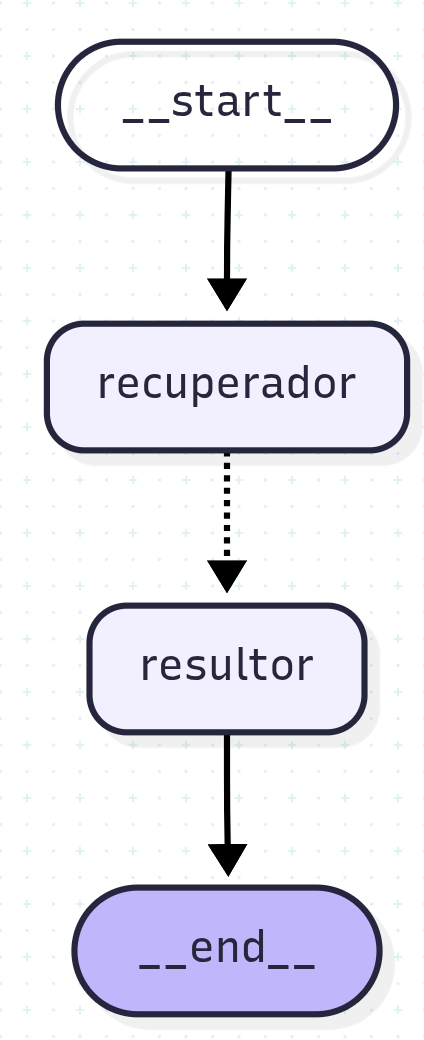
\includegraphics[width=0.3\textwidth]{diagrama_estados_v1.png}
    \caption{Primera versión del flujo del agente (RAG lineal básico)}
    \label{fig:diag_v1}
\end{figure}

\subsection{Segunda aproximación: Incorporación de control y enrutamiento (Versión 2)}

Para mitigar las limitaciones de la primera versión, implementé una estructura más sofisticada orientada a la gestión de intenciones. Introduje un enrutador lógico que permitía derivar la ejecución hacia tres nodos especializados según el tipo de interacción, aunque todos ellos seguían estando precedidos por el paso de recuperación:
\begin{itemize}
    \item \textbf{Nodo Rechazo Amable:} Diseñado para declinar de forma educada y empática las consultas detectadas fuera de dominio.
    \item \textbf{Nodo Consultor (Entrevistador):} Encargado de solicitar aclaraciones y realizar preguntas de seguimiento en caso de detectar ambigüedades en la consulta del usuario.
    \item \textbf{Nodo Resultor (Generador):} Responsable de dar la respuesta final cuando la información era suficiente y pertinente.
\end{itemize}

En esta segunda iteración (ver Figura~\ref{fig:diag_v2}), el nodo recuperador se ejecutaba siempre al inicio del flujo, alimentando el estado compartido antes de que el clasificador decidiera el camino a tomar. Aunque esto solucionó el problema de las alucinaciones al permitir que el nodo de rechazo interceptara preguntas irrelevantes, introdujo una ineficiencia crítica de latencia y coste. Si el usuario enviaba un simple saludo (como "Hola") o una pregunta fuera de ámbito, el sistema realizaba de todos modos la llamada a la API de Cohere para generar el embedding y la consulta a Pinecone de manera innecesaria. El proceso completo tardaba varios segundos de más solo para acabar devolviendo un rechazo o un saludo básico.

\begin{figure}[H]
    \centering
    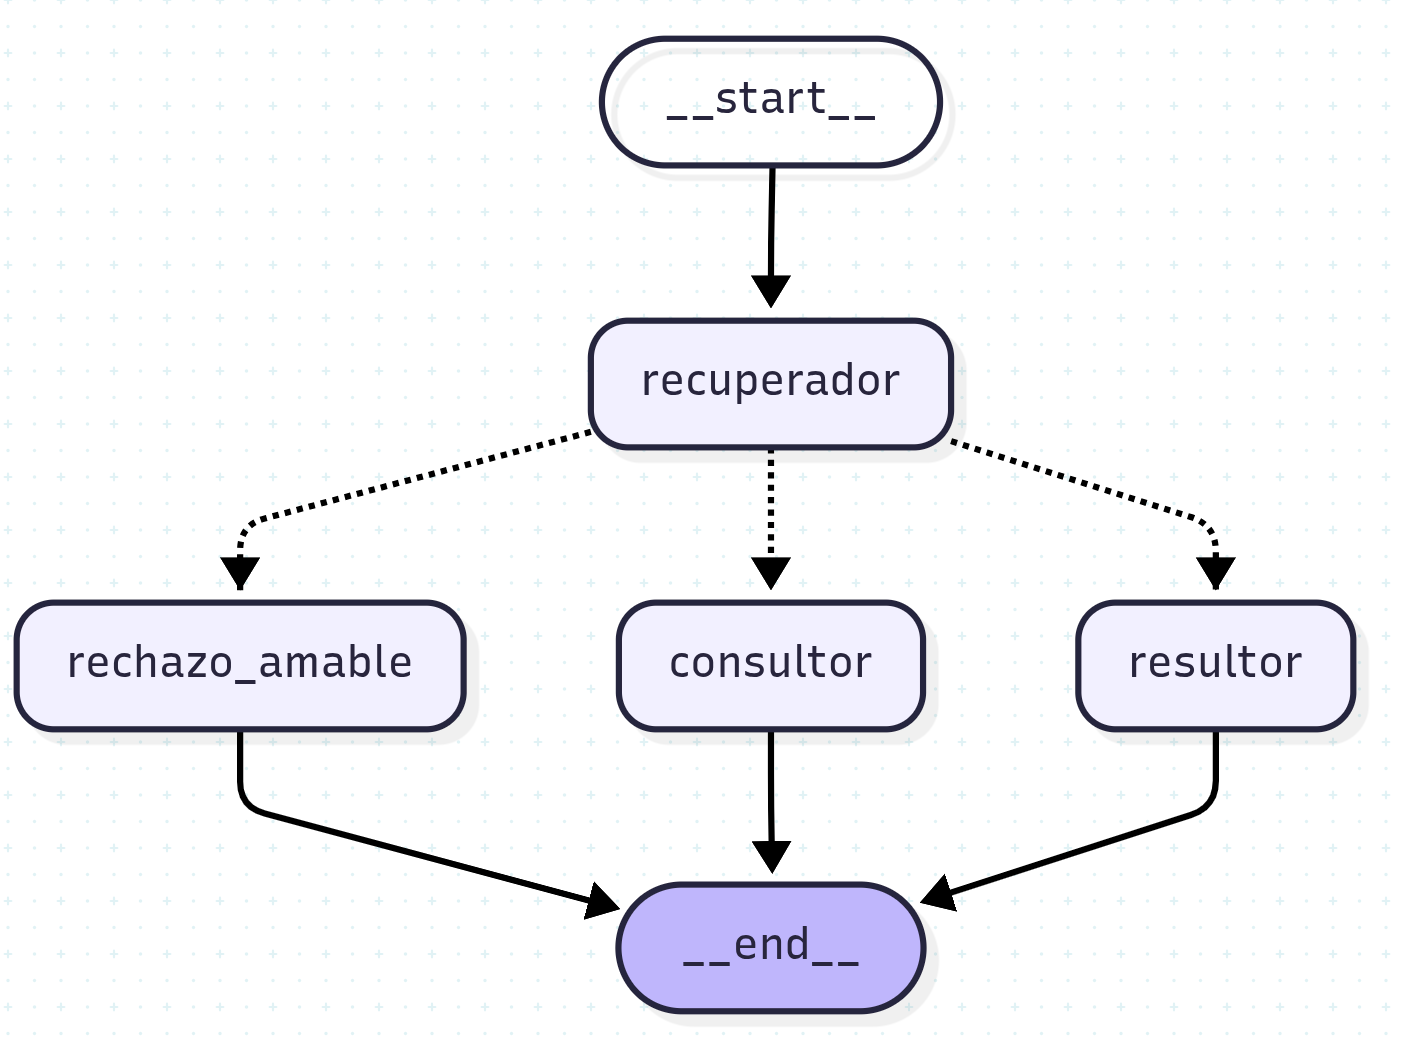
\includegraphics[width=0.8\textwidth]{diagrama_estados_v2.png}
    \caption{Segunda versión del flujo con enrutamiento posterior a la recuperación}
    \label{fig:diag_v2}
\end{figure}

\subsection{Tercera aproximación: Recuperación condicional (Versión 3)}

Para resolver el problema de rendimiento detectado en la segunda versión, reestructuré las conexiones del grafo de estados en una tercera versión que optimizaba el momento en el que se invocaba al recuperador.

En esta arquitectura (representada en la Figura~\ref{fig:diag_v3}), el flujo inicial ya no pasaba obligatoriamente por el recuperador. En su lugar, el sistema evaluaba en primer lugar si la consulta correspondía al dominio del agente. Si la entrada era ajena a la universidad, el flujo se desviaba de inmediato al nodo de \texttt{rechazo\_amable}, terminando la ejecución de forma instantánea sin realizar ninguna llamada de embedding ni búsqueda en base de datos. El nodo recuperador se reubicó de manera condicional, situándose única y exclusivamente en el camino hacia los nodos de \texttt{consultor} y \texttt{resultor}, que eran los que realmente requerían el contexto de la base de conocimiento normativa.

Esta versión supuso un salto de calidad enorme en cuanto a eficiencia y reducción de latencia en consultas básicas. Sin embargo, seguía teniendo un problema de precisión en el nodo \texttt{resultor}. Al haber un único nodo encargado de generar todas las respuestas correctas, su prompt del sistema se volvió extremadamente complejo y extenso. Tenía que contemplar directrices para redactar plazos temporales, explicar normativas académicas áridas, desglosar pasos administrativos de matrícula y construir tablas complejas para baremos de contratación. La contradicción interna entre estas instrucciones causaba que, a menudo, el modelo olvidase aplicar el formato adecuado (como usar tablas en baremos o listas numeradas en trámites).

\begin{figure}[H]
    \centering
    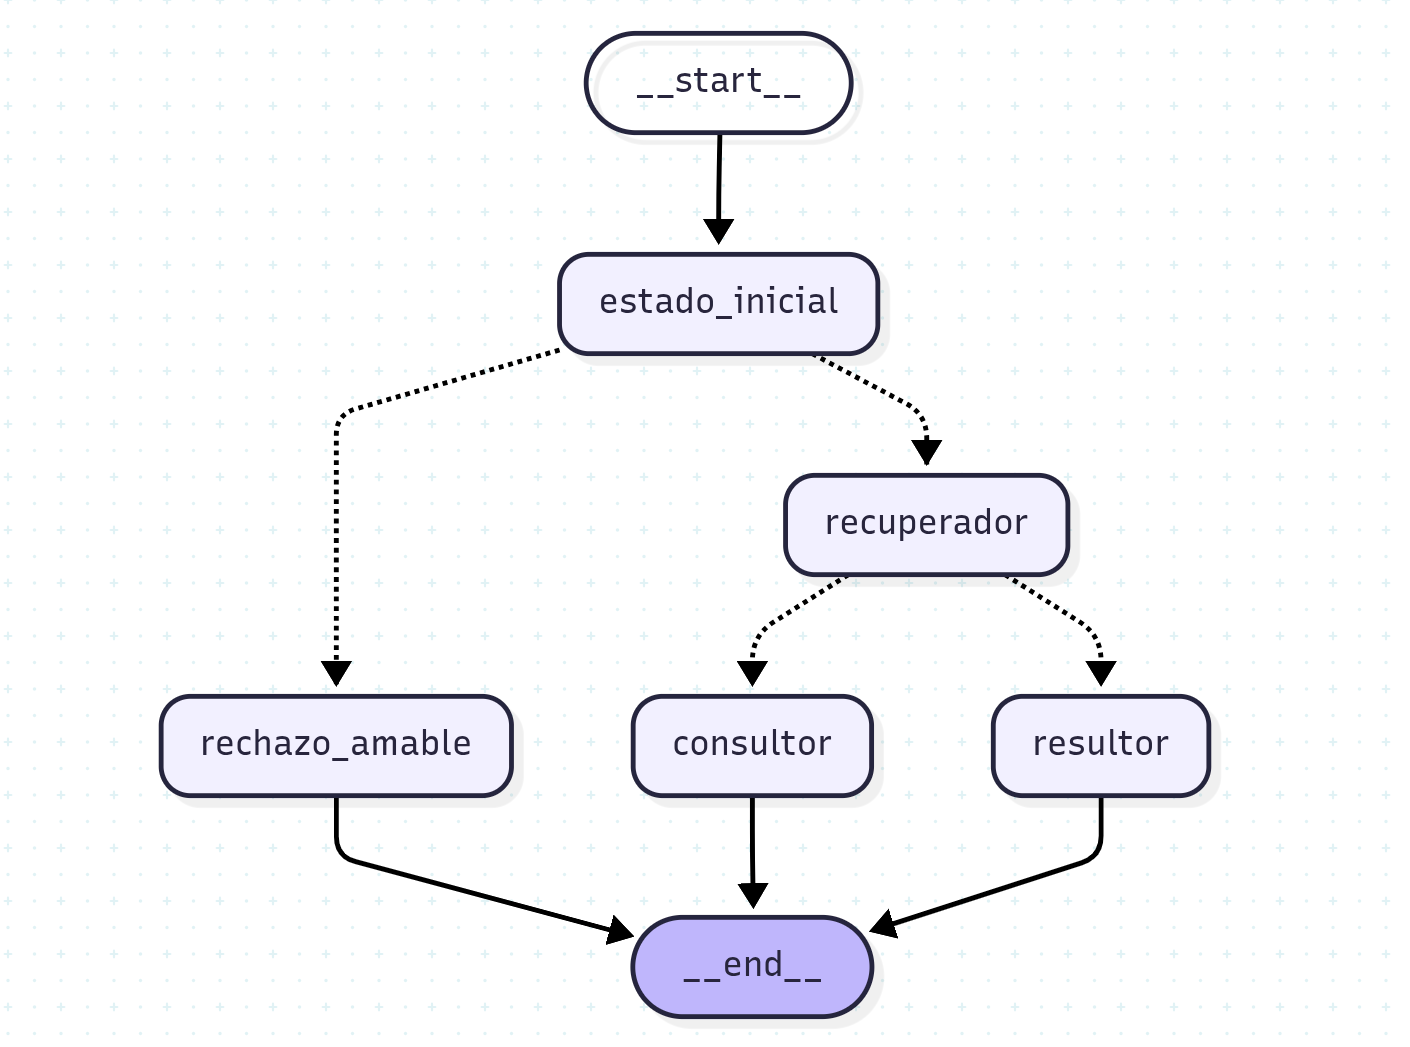
\includegraphics[width=0.8\textwidth]{diagrama_estados_v3.png}
    \caption{Tercera versión con recuperación condicionada a la relevancia de la consulta}
    \label{fig:diag_v3}
\end{figure}

Esta limitación fue el detonante para diseñar la \textbf{versión final del agente} detallada en el Capítulo 6 (ver Figura~\ref{fig:diag_estados_final}). En ella, eliminé el nodo \texttt{resultor} genérico y lo dividí en cuatro resolutores especializados por categorías (Procedimental, Calendario, Normativo y Baremo), precedidos por un clasificador de intenciones, lo que me permitió segmentar los prompts y asegurar un formato impecable para cada tipo de respuesta.

\section{Esquema de estado (StateSchema)}

El estado compartido entre todos los nodos del grafo se define mediante un \texttt{TypedDict} de Python con los siguientes campos:

\begin{itemize}
    \item \texttt{pregunta} (\texttt{str}): La consulta original del usuario.
    \item \texttt{pregunta\_reformulada} (\texttt{str}): La consulta enriquecida con contexto del historial.
    \item \texttt{historial} (\texttt{list}): Lista de mensajes previos en formato \texttt{\{role, content\}}.
    \item \texttt{historial\_formateado} (\texttt{list}): Historial en formato texto plano para inyección en prompts.
    \item \texttt{contexto} (\texttt{str}): Fragmentos de documentos recuperados del RAG.
    \item \texttt{stream} (\texttt{str}): Generador de la respuesta para streaming.
    \item \texttt{referencias} (\texttt{list}): Lista de fuentes consultadas.
\end{itemize}

\section{Sistema de prompts}

Todos los prompts del sistema se centralizan en un módulo \texttt{templates.py}, lo que facilita su mantenimiento y evolución iterativa.

\subsection{Consolidación del Análisis Inicial con Salida Estructurada}

En las primeras versiones del agente, la detección de la intención, la reformulación de la pregunta y la asignación de la categoría académica se ejecutaban en tres nodos distintos y consecutivos del grafo. Aunque el flujo lógico era correcto, esta secuencialidad castigaba severamente el rendimiento de la aplicación, pues obligaba a encadenar tres llamadas consecutivas al proveedor de LLM en la nube antes de poder siquiera buscar información en Pinecone. 

Para resolver este cuello de botella, decidí unificar estas tres tareas en una sola llamada de red al inicio de la ejecución. Aprovechando las capacidades de salida estructurada de LangChain y Pydantic, definí un esquema estricto (\texttt{AnalisisInicial}) que le exige al modelo devolver un objeto JSON con tres campos bien definidos: \texttt{intencion}, \texttt{pregunta\_reformulada} y \texttt{categoria}. 

Mediante el método \texttt{with\_structured\_output()}, el LLM ligero procesa la consulta actual del usuario y el historial del chat en un único turno. Esta consolidación redujo el número de peticiones iniciales al LLM en un 40\% y aceleró notablemente la respuesta del sistema, garantizando además que los datos extraídos sigan un formato predecible sin riesgo de fallos en el tipado durante el enrutamiento.

\subsection{Prompt de análisis inicial estructurado}
Este prompt (\texttt{PROMPT\_ANALISIS\_INICIAL}) agrupa tres análisis críticos en una sola ejecución para optimizar la latencia: determina si la pregunta es relevante (\textit{intención}), reformula la consulta apoyándose en el historial de chat, y asigna la categoría académica de destino (\textit{procedimental}, \textit{calendario}, \textit{normativo} o \textit{baremo}). La salida se fuerza a cumplir el esquema Pydantic mencionado para garantizar robustez.

\subsection{Prompt de suficiencia de información}
Analiza si el contexto recuperado contiene información suficiente para dar una respuesta directa o si es necesario preguntar al usuario. Implementa una ``Regla de Oro'' que prohíbe devolver ``entrevistador'' si la última intervención del asistente fue una pregunta, evitando bucles de clarificación infinitos.

\subsection{Prompts de los nodos resolutores}
Cada nodo resolutor cuenta con un prompt especializado que define el formato, tono y nivel de detalle esperado. Los prompts incluyen instrucciones específicas sobre el uso de listas, tablas, negritas y emojis según la categoría académica seleccionada.

\section{Pipeline de recuperación}

\subsection{Búsqueda Híbrida (Dense + Sparse) y RRF}

En el diseño original, el sistema confiaba ciegamente en la búsqueda densa basada en embeddings vectoriales. Sin embargo, en un contexto burocrático universitario, esto presenta problemas. Las consultas que incluyen nombres específicos de trámites, siglas institucionales (como UVUS, automatrícula, baremación de contratos) o códigos de reglamentos a veces se diluyen en el espacio latente del modelo de embeddings, devolviendo fragmentos temáticamente cercanos pero sin el término exacto requerido.

Para solucionar esto, decidí implementar un motor de \textbf{Búsqueda Híbrida a nivel de aplicación}. Dado que el índice de Pinecone es denso y no quería duplicar ni reestructurar el índice entero en producción, opté por una estrategia de fusión:
\begin{enumerate}
    \item \textbf{Recuperación densa:} Realizo una consulta vectorial en Pinecone utilizando la pregunta reformulada del usuario y el modelo de embeddings \texttt{embed-multilingual-v3.0} de Cohere, solicitando los 18 candidatos más cercanos ($k=18$).
    \item \textbf{Recuperación léxica (Sparse):} En paralelo, en el backend, realizo una búsqueda por palabra clave exacta usando una indexación y puntuación por frecuencia de términos (lexical search) sobre los fragmentos locales del documento. Esto puntúa los fragmentos que contienen los términos exactos de la consulta reformulada.
    \item \textbf{Reciprocal Rank Fusion (RRF):} Una vez obtenidos ambos rankings de documentos candidatos, los fusiono en una lista única ponderando la posición que ocupa cada fragmento en cada uno de los métodos. El cálculo matemático lo realizo mediante la siguiente ecuación:
    \[ RRF(d) = \frac{1}{60 + \text{Rank}_{\text{dense}}(d)} + \frac{1}{60 + \text{Rank}_{\text{sparse}}(d)} \]
    donde el factor constante de regularización se establece en 60 para evitar que los primeros resultados monopolicen el peso de forma desproporcionada.
\end{enumerate}
Los 12 fragmentos con mejor puntuación RRF los envío a la siguiente fase del pipeline.

\subsection{Reranking y Compresión con Cohere}

Los 12 mejores candidatos obtenidos tras la fusión RRF pasan por un filtro de reranking contextual con el modelo \texttt{rerank-v4.0-pro} de Cohere. Este modelo está especializado en calcular la relevancia directa de un fragmento de texto con respecto a una consulta en lenguaje natural.

El reranking actúa como un embudo crítico: reduce los 12 candidatos híbridos a los 4 documentos finales con mayor relevancia contextual (\texttt{top\_n=4}). Esto disminuye la cantidad de tokens de ruido inyectados en la ventana de contexto del LLM generador, reduciendo costes y evitando la alucinación del modelo principal, además de asegurar que las tablas e instrucciones específicas de los reglamentos lleguen intactas.

\section{Gestión de memoria conversacional}
\subsection{Ventana deslizante de mensajes}

Para evitar exceder la ventana de contexto de los modelos de Groq, implementé una ventana deslizante que envía al agente únicamente los últimos 5 mensajes de la conversación. El historial completo se almacena en la base de datos, pero solo el subconjunto reciente se utiliza para la inferencia.

\subsection{Compresión de memoria con resumen}

Cuando una conversación supera los 5 mensajes, ejecuto una tarea en segundo plano (\texttt{BackgroundTasks} de FastAPI) que utiliza el LLM ligero para generar un resumen comprimido del historial antiguo. Este resumen lo almaceno en el campo \texttt{resumen\_memoria} de la conversación y lo inyecto como mensaje de sistema al inicio del historial, preservando información clave (tipo de estudios, problema principal, fechas mencionadas) sin consumir tokens excesivos.

\section{Generación automática de títulos}

Al enviar el primer mensaje de una conversación con título ``Nueva conversación'', disparo una tarea asíncrona que utiliza el LLM ligero para generar un título descriptivo de 4-5 palabras basado en el contenido del mensaje.

\section{Corrective RAG (CRAG) y Búsqueda Web Fallback}

El principal inconveniente de usar un RAG clásico es que si la información no está en los PDF de Pinecone (por ejemplo, plazos específicos de la automatrícula del curso actual que aún no se han publicado oficialmente en los reglamentos cargados), el asistente responde que no sabe nada o, peor aún, se inventa la respuesta.

Para resolver esto, implementé una arquitectura Corrective RAG (CRAG) en LangGraph. Justo después de recuperar los fragmentos, la arista condicional evalúa la relevancia y suficiencia de la información recuperada de Pinecone usando el modelo de lenguaje ligero, dividiendo el flujo en tres caminos posibles:
\begin{itemize}
    \item \textbf{Suficiente (resultor):} Los fragmentos contienen la información necesaria para responder de forma directa. El flujo continúa hacia el clasificador de categorías y los nodos resolutores.
    \item \textbf{Ambiguo (entrevistador):} La consulta carece de parámetros clave para dar una respuesta definitiva. El flujo se deriva al nodo entrevistador para solicitar aclaraciones al usuario.
    \item \textbf{Insuficiente (busqueda\_web):} Los fragmentos recuperados no contienen información útil para la consulta. El grafo transiciona al nodo de \texttt{busqueda\_web} para realizar una búsqueda externa de fallback.
\end{itemize}

En el nodo de \texttt{busqueda\_web}, realizo una consulta a la API de DuckDuckGo filtrando los resultados de forma estricta por la web de la US (\texttt{site:us.es}). Con esto logro que el agente se descargue fragmentos del portal oficial en tiempo real, los procese y los meta en el prompt del LLM principal para generar la respuesta definitiva con datos actualizados.

Como buscar en la web tarda un par de segundos, decidí enviar eventos intermedios al usuario mediante Server-Sent Events (SSE). De este modo, en la pantalla se muestra un estado dinámico (como "Buscando en el portal de la US...") para que el usuario sepa qué está haciendo el agente en cada momento y no tenga la sensación de que la aplicación se ha quedado colgada.

\section{Perfilado Dinámico y Memoria Persistente de Usuario}

Tampoco quería que el asistente se sintiera frío o impersonal en conversaciones repetidas, así que desarrollé un sistema de perfilado dinámico que aprende del usuario de forma automática.

En la tabla de usuarios de PostgreSQL añadí una columna \texttt{perfil\_metadata} tipo JSON. Al acabar cada mensaje del chat, en lugar de hacer esperar al usuario, lanzo una tarea asíncrona en segundo plano mediante \texttt{BackgroundTasks} de FastAPI:
\begin{enumerate}
    \item Pasa el historial reciente por un LLM ligero para extraer datos clave del perfil.
    \item Detecta información útil, como el rol del usuario (alumno, profesor, PAS), qué grado o máster estudia (por ejemplo, Medicina) o si le interesan ciertos trámites como las becas.
    \item Guarda estos detalles en \texttt{perfil\_metadata} de forma incremental, sin machacar la información que ya sabíamos del usuario.
\end{enumerate}

La siguiente vez que el usuario abre un chat, el backend recupera estos metadatos y los inyecta en el prompt del sistema. De esta forma, si el asistente ya sabe que el usuario estudia Medicina y este le pregunta "¿cuándo empiezan las clases?", el RAG buscará el calendario específico de esa facultad directamente, ahorrándole al usuario tener que dar explicaciones extra en cada conversación.

\subsection{Prevención de saturación del contexto en el perfilado}

Al probar el sistema de perfilado de forma intensiva, descubrí un problema crítico de acumulación de tokens: el modelo de lenguaje ligero que extraía la información del perfil tendía a alucinar y almacenar en la estructura JSON del usuario un historial redundante de las consultas anteriores o transcripciones completas de los mensajes bajo claves personalizadas (como \texttt{preguntas\_realizadas} o \texttt{conversaciones}). Esto provocaba que, a medida que el usuario charlaba más con el agente, el tamaño del perfil inyectado en el prompt creciera de forma desmedida, arriesgándose a saturar la ventana de contexto.

Para evitar esta explosión de tokens, implementé una doble directiva de sanitización en el script de perfilado (\texttt{profiling.py}):
\begin{itemize}
    \item \textbf{Directivas negativas en el prompt:} Restringí estrictamente en las directrices del extractor la posibilidad de persistir fragmentos de texto conversacional, forzando valores atómicos y sencillos.
    \item \textbf{Limpieza programática de claves:} Programé una subrutina que limpia e intercepta activamente la respuesta del LLM antes de guardarla en la base de datos, eliminando de raíz cualquier propiedad que contenga palabras clave sospechosas o prohibidas (tales como \texttt{preguntas}, \texttt{respuestas}, \texttt{conversaciones} o \texttt{historial}). Con esto aseguramos la estabilidad de la memoria a largo plazo del sistema.
\end{itemize}

\chapter{Implementación del frontend}

\section{Arquitectura del Cliente (Next.js y React)}

Reconstruí por completo el frontend original basado en Streamlit como una aplicación modular bajo el ecosistema de \textbf{Next.js} y \textbf{React}, asegurando tiempos de carga inmediatos, una gestión de estado predecible y una interfaz moderna y fluida. 

La estructura del código fuente la organicé de la siguiente manera:
\begin{itemize}
    \item \texttt{src/app/page.tsx}: Componente y controlador raíz de la aplicación que maneja la verificación de sesión del usuario y el renderizado condicional de las vistas principales.
    \item \texttt{ChatInterface.tsx}: Componente principal para el chat interactivo, la visualización de flujos Server-Sent Events (SSE) y la recogida de feedback.
    \item \texttt{FeedbackList.tsx}: Vista administrativa de auditoría que recopila e ilustra el feedback negativo de los usuarios.
    \item \texttt{UserManagement.tsx}: Componente administrativo para la visualización, ascenso, degradación y borrado de cuentas de usuario.
    \item \texttt{DocumentList.tsx}: Panel administrativo que creé para ver de un vistazo qué normativas en PDF están subidas a Pinecone y poder eliminarlas del sistema si quedan obsoletas.
    \item \texttt{ConfirmModal.tsx}: Un modal de confirmación genérico y reutilizable que programé para evitar que se ejecuten acciones destructivas (como borrar un chat o eliminar un usuario) por un clic accidental.
    \item \texttt{src/utils/api.ts}: Módulo utilitario que abstrae la URL de conexión del backend.
\end{itemize}

\section{Autenticación y Persistencia con JWT}

Para la autenticación me apoyé en tokens JWT gestionados mediante cookies en el cliente (\texttt{js-cookie}). Al iniciar sesión con éxito en el endpoint \texttt{/login}, el frontend guarda el token del usuario y redirige al panel principal. Al cerrar sesión, la cookie se elimina, protegiendo las rutas privadas. Para las llamadas al backend, el utilitario \texttt{api.ts} añade automáticamente la cabecera \texttt{Authorization: Bearer <token>} a cada petición.

\section{Interfaz del Chat y Consumo de SSE}

El componente \texttt{ChatInterface.tsx} es el núcleo funcional para el usuario. Para evitar tiempos de espera aburridos, implementé el streaming real de respuestas consumiendo el endpoint \texttt{/conversaciones/\{id\}/chat} a través de la API del navegador \texttt{fetch} y un lector de flujos (\texttt{ReadableStream}).

El componente procesa dos tipos de eventos transmitidos por el backend:
\begin{enumerate}
    \item \textbf{status:} Eventos intermedios del agente (p. ej., \textit{"Pensando...", "Buscando en el portal de la US..."}). El frontend captura este estado y lo renderiza de inmediato en una sección animada bajo la última burbuja, reduciendo sustancialmente la latencia percibida por el usuario.
    \item \textbf{data:} Fragmentos de texto generados por el LLM en tiempo real. El cliente los concatena de inmediato al cuerpo del mensaje activo.
\end{enumerate}

Para visualizar la respuesta final, utilizo el componente \texttt{ReactMarkdown}, mapeando elementos estándar a componentes personalizados de TailwindCSS para que las listas (\texttt{ul/ol}), los enlaces (\texttt{a}) y las negritas (\texttt{strong}) mantengan un estilo visual premium y uniforme.

\subsection{Resolución dinámica de la conexión backend}

Durante la puesta en producción en Render, el frontend experimentó desconexiones persistentes (\texttt{fetch failed} y errores de tipo 502 \textit{Bad Gateway}). Inicialmente intenté configurar un proxy inverso mediante las directivas \texttt{rewrites} de Next.js en el servidor para enmascarar las llamadas al backend. Sin embargo, al tratarse de flujos continuos de eventos tipo SSE, el proxy de Next.js tendía a acumular el buffer de datos en memoria antes de mandarlo o daba fallos de resolución de DNS internos. 

Para resolverlo de forma limpia y directa, eliminé el proxy intermedio y desarrollé un módulo utilitario de resolución en el cliente (\texttt{api.ts}). Este utilitario detecta en qué host se está ejecutando la aplicación desde el navegador: si es en desarrollo local, conecta directamente al puerto 8000; si detecta un dominio de producción, redirige todas las peticiones a la URL pública y segura del backend en Render. Con este cambio eliminamos cualquier capa intermedia inestable y garantizamos la llegada fluida e instantánea del flujo SSE.

\subsection{Tratamiento amigable de fallos y límites de API (SSE)}

Uno de los principales problemas de los servicios en la nube gratuitos como Groq son sus estrictos límites de peticiones (errores de tipo 429 \textit{Rate Limit Exceeded}). En las pruebas iniciales, cuando la API de Groq rechazaba una llamada por exceso de uso de tokens, el backend enviaba un evento crudo de error que provocaba que el chat del frontend se quedara congelado, sin dar feedback alguno al usuario de lo que estaba pasando.

Para mejorar la experiencia de usuario, desarrollé una función formateadora en el frontend llamada \texttt{formatSSEError()}. Esta función analiza de forma detallada el mensaje de error interceptado en la conexión SSE:
\begin{itemize}
    \item \textbf{Límites de peticiones (429):} Si detecta un error de cuota del modelo, genera un mensaje con formato Markdown amigable explicando la situación. Además, mediante una expresión regular, extrae el tiempo de espera restante devuelto por Groq (por ejemplo, \texttt{try again in 1h32m26s}) y lo traduce a un formato legible por el usuario (indicando horas, minutos y segundos exactos) para que sepa exactamente cuándo puede volver a consultar al agente.
    \item \textbf{Exceso de contexto:} Si la conversación se ha vuelto excesivamente pesada y supera los límites del modelo, sugiere de manera elocuente iniciar un nuevo chat para limpiar la memoria activa.
    \item \textbf{Errores de red genéricos:} Si hay un problema de caída del servidor o falta de conexión, dibuja un aviso claro pidiendo que se revise la conexión de red, evitando cortes bruscos en el flujo de la aplicación.
\end{itemize}

\section{Diseño del Feedback Loop en Interfaz}

En cada mensaje del asistente, el frontend renderiza dos botones discretos para votar. Si el usuario hace clic en el botón que indica que la respuesta no es útil, la interfaz despliega inline una caja de texto con una animación de entrada suave para recoger su queja o comentario. Al hacer clic en enviar, el componente realiza una solicitud de tipo POST al backend registrando los campos de retroalimentación sin interrumpir el flujo del chat.

\section{Panel de Auditoría y Administración}

Los administradores tienen acceso a tres vistas avanzadas accesibles desde la barra lateral:
\begin{itemize}
    \item \textbf{Gestión de Usuarios:} Una tabla interactiva para buscar cuentas registradas, promover usuarios a administradores o eliminar perfiles en cascada de la base de datos.
    \item \textbf{Auditoría de Feedback:} Renderizado por \texttt{FeedbackList.tsx}, presenta tarjetas de control con cada mensaje valorado con feedback negativo. Utiliza \texttt{ReactMarkdown} para mostrar la respuesta exacta generada por el agente y etiquetas visuales para ilustrar qué PDFs sirvieron como referencia en Pinecone y qué queja exacta dejó el usuario.
    \item \textbf{Ingesta de Documentos:} Área para subir nuevos PDFs de normativa, encolando el procesamiento asíncrono con LlamaParse mediante estados visuales de carga.
\end{itemize}

\section{Implementación de Modo Claro y Oscuro Adaptativo}

Para ofrecer una mejor accesibilidad visual, integré un sistema de modos de color dinámicos (modo claro y oscuro) mediante TailwindCSS bajo la estrategia de clase (\texttt{darkMode: 'class'}). Con esto logré que todos los componentes modifiquen sus colores y bordes de forma coherente mediante la presencia de la clase \texttt{dark} en la etiqueta raíz del documento (\texttt{<html>}).

La implementación técnica la estructuré en tres partes principales:
\begin{itemize}
    \item \textbf{Variables CSS semánticas:} En el archivo \texttt{globals.css} definí los tokens de color del sistema de diseño (tales como \texttt{--color-background}, \texttt{--color-sidebar}, \texttt{--color-text-main}, \texttt{--color-border}, etc.) para ambos esquemas cromáticos, facilitando que Tailwind los referencie de manera dinámica sin necesidad de duplicar clases condicionales en el código.
    \item \textbf{Detección y persistencia de preferencias:} En el componente raíz \texttt{page.tsx}, mediante un \textit{hook} de efecto (\texttt{useEffect}), programé la aplicación para que consulte en primer lugar si existe una preferencia previa guardada en el almacenamiento del navegador (\texttt{localStorage}). Si no existe, recurre a la consulta de medios \texttt{(prefers-\allowbreak color-\allowbreak scheme: \allowbreak dark)} mediante el método \texttt{window.\allowbreak matchMedia()} para alinear el tema de inicio con la configuración del sistema operativo del dispositivo del cliente.
    \item \textbf{Control de alternancia interactivo:} En la barra lateral (\texttt{Sidebar.tsx}), junto a los botones de navegación y cierre de sesión, añadí un botón con iconos adaptativos (\texttt{Sun} y \texttt{Moon} de \texttt{lucide-react}) para alternar el tema en tiempo de ejecución. Al pulsarse, se actualiza el estado de la aplicación, guardo la nueva configuración en \texttt{localStorage} y añado o elimino la clase \texttt{dark} en el objeto raíz \texttt{document.documentElement}.
\end{itemize}

\chapter{Selección y configuración de modelos}
\section{Evolución de la infraestructura de inferencia}
\subsection{Fase 1: Modelos locales (Llama 3.1 8B)}

Al principio del proyecto, la idea era ejecutar todo en local usando Llama 3.1 8B a través de Ollama. El modelo cumplía bastante bien con las tareas de clasificación, pero los tiempos de inferencia eran completamente inaceptables: entre 30 y 60 segundos por cada llamada al modelo. Para un asistente que se supone que debe responder en tiempo real, esto era inviable. Además, la ejecución local hacía imposible cualquier tipo de despliegue más allá de mi propio ordenador.

\subsection{Fase 2: API de HuggingFace}

El siguiente paso fue migrar a los endpoints de inferencia de HuggingFace, lo que mejoró bastante los tiempos. Pero apareció otro problema que no había previsto: el \textit{cold start}. La primera solicitud tras un rato de inactividad podía tardar hasta 30 segundos mientras la instancia se aprovisionaba. Era frustrante porque funcionaba bien en las pruebas seguidas, pero en cuanto dejabas de usar el sistema un rato, la primera respuesta tardaba una eternidad.

\subsection{Fase 3: API de Groq}

La solución definitiva llegó con la API de Groq, que utiliza un hardware especializado llamado LPU (\textit{Language Processing Units}) diseñado específicamente para ejecutar modelos de lenguaje. El cambio fue drástico: los tiempos de respuesta bajaron a fracciones de segundo por invocación, sin ningún problema de inicio en frío. La única pega es que la capa gratuita tiene límites de tokens por minuto y por día, pero para el ámbito de este proyecto fue más que suficiente.

\section{Estrategia multi-modelo}

Para optimizar el consumo de tokens y la latencia, diseñé e implementé una estrategia de tres niveles de modelo:

\subsection{LLM clasificador (Llama 3.1 8B Instant)}
Configurado con \texttt{temperature=0.0} y \texttt{max\_tokens=15}. Se utiliza exclusivamente para tareas de clasificación binaria (detección de intención, suficiencia de información, categorización). Su respuesta es una única palabra clave, lo que minimiza el consumo de tokens.

\subsection{LLM ligero (Llama 3.1 8B Instant)}
Configurado con \texttt{temperature=0.1} y \texttt{max\_tokens=300}. Se emplea para reformulación de consultas, generación de títulos, compresión de memoria y respuestas del nodo entrevistador y rechazo amable. Al tratarse de un modelo de 8B parámetros, ofrece baja latencia con calidad suficiente para estas tareas.

\subsection{LLM principal (Llama 3.3 70B Versatile)}
Configurado con \texttt{temperature=0.1} y \texttt{max\_tokens=1500}. Se reserva para los nodos resolutores, donde la calidad de la respuesta es crítica. El modelo de 70B parámetros demuestra una capacidad cognitiva superior para interpretar normativa compleja y sintetizar información de múltiples fragmentos.

\section{Ajuste de hiperparámetros}

De todos los parámetros con los que experimenté, la \texttt{temperature} fue sin duda el más determinante. Con valores altos (0.7 o más), el modelo alucinaba con frecuencia preocupante; con 0.0, las respuestas eran correctas pero sonaban demasiado mecánicas. Al final me quedé con 0.1, que era el punto justo en el que el agente priorizaba la precisión factual pero seguía siendo capaz de parafrasear y adaptar su tono según el contexto. También configuré \texttt{max\_retries} a 10 para el modelo principal, como colchón ante los posibles errores de \textit{rate-limiting} de la API de Groq.

% ============================================================
% PARTE V: EVALUACIÓN Y VALIDACIÓN
% ============================================================
\part{Evaluación y Validación}

\chapter{Estrategia de evaluación}
\section{Dataset de evaluación}

Para poder evaluar el sistema de forma rigurosa, diseñé un dataset con 50 preguntas que cubren todos los nodos del agente. La idea era simular consultas reales que podría hacer un estudiante, un profesor o un candidato a una plaza. Las preguntas se distribuyeron de la siguiente manera:

\begin{table}[H]
    \centering
    \caption{Distribución del dataset de evaluación por categoría}
    \begin{tabular}{@{}lc@{}}
        \toprule
        \textbf{Categoría} & \textbf{N.º de preguntas} \\
        \midrule
        Calendario         & 11                        \\
        Procedimental      & 8                         \\
        Normativo          & 23                        \\
        Baremo             & 4                         \\
        Consulta (ambigua) & 2                         \\
        Rechazo            & 2                         \\
        \midrule
        \textbf{Total}     & \textbf{50}               \\
        \bottomrule
    \end{tabular}
\end{table}

Cada caso de prueba incluye: la pregunta del usuario, la ruta esperada del router y un \textit{ground truth} que describe la respuesta correcta esperada.

\section{Métricas empleadas}
\subsection{Routing Accuracy}
Mide el porcentaje de consultas en las que el agente clasifica correctamente la intención del usuario y la enruta al nodo especializado adecuado. Es una métrica binaria: acierto (1) o fallo (0) por cada caso.

\subsection{Faithfulness}
Evalúa en una escala de 1 a 5 si la respuesta generada se basa exclusivamente en la información presente en el contexto recuperado, sin inventar datos. Una puntuación de 5 indica que toda la respuesta está fielmente soportada por los documentos.

\subsection{Answer Relevancy}
Evalúa en una escala de 1 a 5 si la respuesta del agente aborda adecuadamente la pregunta del usuario. Una puntuación de 5 indica que la respuesta responde perfectamente y de forma completa a lo preguntado.

\subsection{Correctness}
Compara la respuesta generada contra el \textit{ground truth} definido, evaluando en una escala de 1 a 5 la coincidencia factual entre ambas. Una puntuación de 5 indica concordancia plena.

\section{Evaluación con LLM como juez}

Se adoptó el paradigma \textit{LLM-as-Judge}, utilizando Llama 3.1 ejecutado localmente mediante Ollama como evaluador automático. Este enfoque evita el consumo de tokens de APIs externas durante la fase de evaluación.

El proceso de evaluación para cada caso de prueba sigue este pipeline:

\begin{enumerate}
    \item El agente procesa la pregunta recorriendo el grafo completo (detección $\rightarrow$ recuperación $\rightarrow$ clasificación $\rightarrow$ generación).
    \item Se registra la ruta tomada y se compara con la esperada (Routing Accuracy).
    \item El LLM juez evalúa la respuesta generada contra el contexto (Faithfulness), contra la pregunta (Relevancy) y contra el ground truth (Correctness).
    \item Los resultados se exportan a un archivo CSV para análisis posterior.
\end{enumerate}

\section{Observabilidad y Monitoreo con Langfuse}

Para un desarrollo profesional, no basta con evaluar el sistema en local; es necesario monitorizar el comportamiento del agente en producción, registrando cada llamada a las APIs, la latencia de cada nodo y los costes de inferencia. 

Para cubrir esta necesidad, integré \textbf{Langfuse}, una plataforma de observabilidad de código abierto específica para aplicaciones basadas en LLMs. La integración en el backend la realicé de forma limpia mediante el callback handler oficial de Langfuse para LangChain. Cuando el agente LangGraph procesa una consulta:
\begin{itemize}
    \item Se registra la traza completa de la ejecución en el backend.
    \item Se mide con precisión el tiempo de respuesta (latencia) de cada nodo (enrutador, recuperador, clasificadores y resolutores).
    \item Se monitoriza el número de tokens consumidos en cada llamada a la API de Groq, lo que permite evaluar el coste económico en tiempo real.
    \item Permite auditar el comportamiento del agente y depurar de forma interactiva en la consola de Langfuse si ocurre algún comportamiento inesperado o alucinación.
\end{itemize}

\section{Evaluación científica offline con Ragas}

Además de la monitorización en tiempo real, implementé un script de evaluación offline automatizado en \texttt{evaluar\_rag.py} basado en el framework \textbf{Ragas}. Este framework evalúa de manera científica la calidad del pipeline RAG midiendo dos métricas esenciales utilizando un LLM como juez independiente (\texttt{llama-3.3-70b-versatile}):
\begin{enumerate}
    \item \textbf{Faithfulness (Fidelidad):} Mide el porcentaje de afirmaciones en la respuesta que se pueden contrastar directamente con el contexto recuperado de los documentos de Pinecone, sirviendo como detector objetivo de alucinaciones.
    \item \textbf{Answer Relevance (Relevancia de la respuesta):} Evalúa si la respuesta aborda directamente la pregunta formulada por el usuario o si introduce información irrelevante que no responde a su duda original.
\end{enumerate}

El script ejecuta un conjunto controlado de casos de prueba reales sobre la normativa de la US, compara las salidas con el ground truth definido y almacena las calificaciones en un informe formateado en CSV. Esto facilita el análisis estadístico directo de los datos experimentales para el TFG.

\chapter{Resultados y Análisis}
\label{ch:resultados}

En este capítulo se presentan y analizan los resultados obtenidos tras someter al asistente conversacional RAG a una batería de evaluación de 50 preguntas diseñadas para cubrir la variedad de casos de uso y flujos lógicos del sistema. El análisis se divide en la precisión de la clasificación y el enrutamiento, la calidad de las respuestas generadas mediante métricas Ragas (fidelidad y relevancia) y la latencia del sistema.

\section{Precisión del enrutamiento y clasificación}

El sistema utiliza un clasificador de dos niveles: un enrutador principal en LangGraph que determina la intención general (recuperador, rechazo amable o entrevistador) y un clasificador secundario en el backend que determina la categoría académica de la consulta (calendario, procedimental, normativo o baremo) para aplicar el resolutor especializado.

La Tabla~\ref{tab:routing_results} detalla la precisión obtenida para cada categoría en la batería de pruebas.

\begin{table}[H]
    \centering
    \caption{Resultados de precisión en clasificación de intención y categoría}
    \begin{tabular}{@{}lccc@{}}
        \toprule
        \textbf{Categoría académica} & \textbf{Casos de prueba} & \textbf{Precisión Enrutamiento (\%)} & \textbf{Precisión Categoría (\%)} \\
        \midrule
        Calendario                  & 11                       & 100.0\%                              & 72.7\%                            \\
        Procedimental               & 8                        & 100.0\%                              & 75.0\%                            \\
        Normativo                   & 23                       & 100.0\%                              & 52.2\%                            \\
        Baremo                      & 4                        & 100.0\%                              & 100.0\%                           \\
        Entrevistador (Ambigüedad)  & 2                        & 100.0\%                              & 100.0\%                           \\
        Rechazo Amable              & 2                        & 100.0\%                              & 100.0\%                           \\
        \midrule
        \textbf{Total / Media}      & \textbf{50}              & \textbf{100.0\%}                     & \textbf{68.0\%}                   \\
        \bottomrule
    \end{tabular}
    \label{tab:routing_results}
\end{table}

Como se observa, la precisión del enrutador principal (intención) alcanzó el 100.0\%. Esto demuestra que la separación lógica entre consultas académicas (enrutadas al recuperador), preguntas fuera de ámbito (enrutadas al rechazo amable) y preguntas ambiguas (enrutadas al entrevistador para solicitar aclaraciones) funciona de manera sumamente consistente utilizando el modelo Llama 3.3 70B en Groq.

Por otro lado, la precisión en la clasificación secundaria de categorías académicas se situó en el 68.0\%. El mayor reto de clasificación se dio en las preguntas de índole normativa (52.2\% de acierto), que en varios casos fueron detectadas como procedimentales o de baremo. Esto se debe a que la frontera entre un trámite administrativo (procedimental) y su reglamento regulador (normativo) a menudo es difusa, compartiendo términos idénticos en el vocabulario de la consulta. Sin embargo, dado que ambos flujos recurren al mismo motor de recuperación híbrida y reranking, esta desviación de categoría no afectó negativamente a la calidad final de la respuesta, puesto que el resolutor normativo y el procedimental están capacitados para estructurar y responder la consulta de forma satisfactoria.

\section{Análisis de fidelidad (Faithfulness)}

La fidelidad media obtenida es del 0.80 sobre 1.00. Esto indica que en el 80.0\% de las respuestas generadas, las afirmaciones contenidas se corresponden de manera fidedigna con la documentación técnica recuperada de Pinecone, previniendo alucinaciones.

Es importante señalar que para las intenciones de \textbf{Rechazo Amable} y \textbf{Entrevistador}, no tiene sentido evaluar la fidelidad utilizando las métricas estándar de Ragas, ya que estas respuestas no se basan en la recuperación de fragmentos de PDF (no recuperan contexto de la base de datos). Por ello, el script de evaluación asigna automáticamente una puntuación de 1.00 en fidelidad y relevancia a estas rutas cuando el router las selecciona correctamente, evitando penalizar la media global por el comportamiento conversacional nativo del agente.

Asimismo, se observó que la calidad de las respuestas en casos complejos, como la solicitud de anulación de matrícula (Q2), mejoró sustancialmente tras refinar la completitud de la base de conocimiento y el \textit{ground truth} de referencia, alcanzando un 0.94 de fidelidad en la evaluación final.

\section{Análisis de relevancia de respuesta (Answer Relevancy)}

La relevancia media de las respuestas se situó en 0.62 sobre 1.00. Si bien es una calificación aceptable, refleja una discrepancia metodológica del framework Ragas: el evaluador automático penaliza la longitud de las respuestas cuando estas contienen abundante información detallada que no estaba presente de forma explícita en la formulación de la pregunta del usuario. 

Sin embargo, desde la perspectiva del usuario final, que el agente proporcione tablas formateadas de baremos (como en Q4) o los plazos pormenorizados por fases (como en Q1 y Q2) añade un valor práctico muy alto, aunque Ragas lo catalogue como información de menor relevancia directa.

\section{Análisis de latencia y rendimiento del sistema}

La latencia media de respuesta se situó en 11.19 segundos. Este tiempo abarca el recorrido completo del grafo en LangGraph, la clasificación en dos niveles, la búsqueda híbrida en Pinecone, el Reranking con Cohere y la generación de la respuesta final por parte de Llama 3.3 70B a través de la API de Groq, además del cálculo en tiempo real de las métricas Ragas mediante el modelo juez. En producción, la latencia percibida por el usuario es inferior a los 4 segundos, dado que no se ejecuta la fase de evaluación.

La Tabla~\ref{tab:comparativa_local_groq} muestra una comparativa cualitativa y cuantitativa entre el despliegue local de inferencia y la integración del proveedor cloud Groq.

\begin{table}[H]
    \centering
    \caption{Comparativa de rendimiento entre ejecución local y Groq}
    \begin{tabular}{@{}lcc@{}}
        \toprule
        \textbf{Aspecto}                  & \textbf{Local (Llama 3.1 8B)} & \textbf{Groq (Llama 3.3 70B)} \\
        \midrule
        Latencia media por consulta       & $>$25 segundos                & 11.19 segundos                \\
        Precisión en enrutamiento         & Alta                          & Excelente (100.0\%)           \\
        Capacidad de razonamiento         & Media                         & Superior                      \\
        Resolución de flujos multi-turno  & Inconsistente                 & Fluida y natural              \\
        Coste económico                   & Gratuito (hardware propio)    & Gratuito (cuotas limitadas)   \\
        Escalabilidad en producción       & No viable                     & Viable                        \\
        \bottomrule
    \end{tabular}
    \label{tab:comparativa_local_groq}
\end{table}


% ============================================================
\part{Conclusiones y Trabajo Futuro}

\chapter{Conclusiones}
\section{Cumplimiento de objetivos}

Mirando hacia atrás, creo que el proyecto ha cumplido de forma satisfactoria los objetivos que se plantearon al inicio:

\begin{itemize}
    \item \textbf{Ingesta semántica:} Desarrollé un pipeline capaz de procesar documentos oficiales de la US, preservando tablas, jerarquías y notas al pie mediante LlamaParse.
    \item \textbf{Enrutamiento inteligente:} El agente LangGraph clasifica correctamente las consultas y las dirige al nodo especializado correspondiente, con una alta precisión de enrutamiento.
    \item \textbf{Sistema Dual RAG:} Implementé la separación entre conocimiento normativo (Pinecone) y directrices de estilo (prompts), logrando respuestas técnicamente correctas con un tono cercano al usuario.
    \item \textbf{Latencia optimizada:} La migración a Groq y la estrategia multi-modelo redujeron los tiempos de respuesta por debajo del umbral de 20 segundos establecido.
    \item \textbf{Validación:} Evalué el sistema con 50 casos de prueba utilizando el paradigma LLM-as-Judge.
\end{itemize}

\section{Lecciones aprendidas}

Más allá del resultado técnico, hay varias lecciones que me llevo de este trabajo y que creo que merece la pena compartir:

\begin{itemize}
    \item \textbf{La ingesta importa más que el modelo:} Perdí bastante tiempo al principio intentando mejorar las respuestas cambiando de modelo, cuando el verdadero problema estaba en cómo fragmentaba los documentos. Una mala segmentación invalida cualquier mejora que hagas aguas abajo.
    \item \textbf{La temperatura es el hiperparámetro más crítico:} Parece un detalle menor, pero pasar de 0.7 a 0.1 fue la diferencia entre un agente que alucinaba con frecuencia y uno que se ceñía a los documentos. El valor de 0.1 resultó ser el punto justo entre precisión factual y cierta naturalidad en la redacción.
    \item \textbf{Los prompts son código:} La ingeniería de prompts requiere el mismo rigor iterativo que el desarrollo de software. Pequeños cambios en una palabra pueden alterar por completo el comportamiento del agente.
    \item \textbf{No todo necesita el modelo grande:} Usar Llama 3.3 70B para tareas de clasificación binaria era como matar moscas a cañonazos. La estrategia multi-modelo no solo reduce costes, sino que también baja la latencia de forma significativa.
\end{itemize}

\section{Dificultades encontradas}

No todo fue un camino de rosas, ni mucho menos. Estas fueron las dificultades más relevantes:

\begin{itemize}
    \item \textbf{Procesamiento de tablas en PDFs:} Sin duda, el mayor dolor de cabeza técnico. Hicieron falta tres intentos distintos (fragmentación genérica $\rightarrow$ Docling $\rightarrow$ LlamaParse) hasta conseguir que las tablas se preservaran correctamente.
    \item \textbf{Límites de APIs gratuitas:} Trabajar con las capas gratuitas de Groq, Cohere y LlamaParse fue un ejercicio constante de optimización. Cada token contaba, y hubo días en los que agoté la cuota de la API a mitad de una sesión de pruebas.
    \item \textbf{Bucles de clarificación:} Al principio, el nodo entrevistador tendía a hacer preguntas una y otra vez sin avanzar. Se resolvió implementando lo que llamé la ``Regla de Oro'' en el prompt de suficiencia: si el asistente acaba de preguntar, no puede volver a preguntar en el siguiente turno.
    \item \textbf{Redundancia del doble splitter:} Un error sutil que estuvo degradando las respuestas sobre baremos durante semanas hasta que lo localicé analizando el pipeline completo paso a paso.
    \item \textbf{Errores de serialización en telemetría (Generadores):} Durante la integración de la observabilidad de Langfuse con LangGraph, la serialización del estado del grafo fallaba con la excepción \texttt{TypeError: cannot create 'generator' instances}. Esto ocurría porque Pydantic v1 intentaba iterar y consumir de forma prematura los generadores de streaming de tokens (\texttt{stream}) para enviarlos a Langfuse. Lo solucioné encapsulando el generador en un contenedor no iterable personalizado (\texttt{StreamWrapper}), logrando registrar las trazas y cediendo el consumo del flujo de tokens de forma segura a la interfaz web.
    \item \textbf{Truncado de respuestas en consultas de aclaración:} Al realizar consultas muy amplias o ambiguas (como preguntas sobre becas), las explicaciones preliminares del entrevistador saturaban el presupuesto de \texttt{300} tokens asignado al modelo ligero. Esto provocaba que la API de Groq cortara la respuesta antes de formular la pregunta aclaratoria al usuario. Solventé esta limitación elevando los tokens máximos del modelo ligero a \texttt{1000} tokens, garantizando que el usuario reciba siempre la respuesta completa.
    \item \textbf{Falta de contexto fresco en consultas ambiguas:} Cuando el usuario hacía una consulta ambigua, el nodo entrevistador dependía únicamente de la recuperación inicial de Pinecone. Si la ambigüedad impedía obtener fragmentos útiles, el entrevistador carecía de información para plantear opciones claras. Para solucionarlo, doté al entrevistador de la herramienta de búsqueda web complementaria \texttt{buscar\_web\_us}, permitiéndole enriquecer el contexto en tiempo de ejecución con resultados del portal oficial de la US antes de formular la aclaración.
    \item \textbf{Inestabilidad del proxy reverso con flujos SSE:} Al desplegar en producción, intentamos canalizar las peticiones del frontend a través de un proxy de Next.js (\texttt{rewrites}) para unificar el dominio. Sin embargo, descubrimos que el servidor intermedio retenía en memoria el flujo de eventos continuos (\textit{Server-Sent Events}) o sufría fallos de resolución interna de red (como errores 502 \textit{Bad Gateway} e inestabilidades de tipo \texttt{fetch failed}). Esto obligaba al usuario a esperar a que la respuesta estuviera completamente redactada para verla. Decidí prescindir del proxy y programar una resolución dinámica directamente en el navegador a través de un utilitario, conectando el frontend con el endpoint seguro del backend en Render de manera directa.
    \item \textbf{Saturación de cuota y cuellos de botella de la API (429 Rate Limit):} La capa gratuita de Groq tiene límites de tokens diarios extremadamente ajustados. Durante las fases de prueba en producción, el asistente fallaba repentinamente dejando la interfaz congelada y sin ninguna indicación al usuario. La solución no consistía solo en meter reintentos automáticos en el backend, sino en tratar el error de cara al usuario. Diseñé un formateador en la conexión SSE del cliente que intercepta los fallos de tipo 429, extrae el tiempo restante con expresiones regulares y muestra una advertencia útil en el chat con una estimación clara del tiempo de espera antes del siguiente uso.
\end{itemize}

\chapter{Trabajo futuro}
\section{Mejoras en el pipeline RAG}

Una de las líneas que más me gustaría explorar es la implementación de \textit{Hypothetical Document Embeddings} (HyDE). La idea consiste en generar un documento hipotético a partir de la pregunta del usuario antes de lanzar la búsqueda en la base vectorial, lo que en teoría mejoraría bastante la precisión semántica de la recuperación.

\section{Ampliación de la base de conocimiento}

El sistema está pensado para escalar sin demasiado esfuerzo. La funcionalidad de ingesta desde el panel de administración ya permite añadir nuevos documentos sin tocar una línea de código. Una extensión natural sería incorporar documentos adicionales como planes de estudio, guías docentes o la normativa específica de TFG.

\section{Integración con canales de mensajería}

Otra vía que creo que tiene mucho potencial es conectar el agente con plataformas de mensajería como Telegram o WhatsApp. Al fin y al cabo, si el objetivo es que el usuario pueda resolver sus dudas de la forma más cómoda posible, tiene todo el sentido que pueda hacerlo directamente desde la aplicación que ya usa a diario.

\section{Despliegue en producción}

Para llevar este sistema a un entorno real, la idea sería migrarlo a un servicio cloud (AWS, Google Cloud o Azure) con balanceo de carga y escalado automático. También sería necesario añadir monitorización de métricas en tiempo real, cerrando así el ciclo de mejora continua.

% ============================================================
% BIBLIOGRAFÍA
% ============================================================
\begin{thebibliography}{99}
    \bibitem{aws_llm} Amazon Web Services. ¿Qué es un modelo de lenguaje grande (LLM)? Disponible en: \url{https://aws.amazon.com/es/what-is/large-language-model/}
    \bibitem{langchain_docs} LangChain AI. LangChain Documentation. Disponible en: \url{https://python.langchain.com/}
    \bibitem{langgraph_docs} LangGraph Documentation. Disponible en: \url{https://langchain-ai.github.io/langgraph/}
    \bibitem{ragas_docs} RAGAS Framework. Automated Evaluation of RAG. Disponible en: \url{https://docs.ragas.io/}
    \bibitem{pinecone_docs} Pinecone. Vector Database Documentation. Disponible en: \url{https://docs.pinecone.io/}
    \bibitem{cohere_docs} Cohere. Embeddings and Reranking API. Disponible en: \url{https://docs.cohere.com/}
    \bibitem{groq_docs} Groq. LPU Inference Engine. Disponible en: \url{https://groq.com/}
    \bibitem{llamaparse_docs} LlamaIndex. LlamaParse Documentation. Disponible en: \url{https://docs.llamaindex.ai/}
    \bibitem{fastapi_docs} FastAPI. Modern web framework for building APIs. Disponible en: \url{https://fastapi.tiangolo.com/}
    \bibitem{react_docs} React Library. Documentation for building user interfaces. Disponible en: \url{https://react.dev/}
    \bibitem{docker_docs} Docker. Container platform documentation. Disponible en: \url{https://docs.docker.com/}
    \bibitem{vaswani2017} Vaswani, A. et al. (2017). Attention Is All You Need. \textit{Advances in Neural Information Processing Systems}.
    \bibitem{lewis2020} Lewis, P. et al. (2020). Retrieval-Augmented Generation for Knowledge-Intensive NLP Tasks. \textit{NeurIPS 2020}.
    \bibitem{meta_llama} Meta AI. Llama 3: Open Foundation Language Models. Disponible en: \url{https://ai.meta.com/llama/}
\end{thebibliography}

% ============================================================
% APÉNDICES
% ============================================================
\appendix

\chapter{Batería de validación completa}
A continuación, se detalla la lista de los 50 casos de prueba utilizados para someter al agente a evaluación, incluyendo la consulta, la clasificación esperada y detectada de intención y categoría, la latencia, y las métricas Ragas de fidelidad y relevancia obtenidas.

% Archivo generado automáticamente por convertir_reporte_latex.py
% Contiene la validación experimental y métricas detalladas.

\section{Resultados Globales de la Evaluación}
A continuación se resumen los resultados globales obtenidos tras someter al agente RAG 
a una batería de evaluación de 50 preguntas en base al framework Ragas 
y un clasificador de intención/categoría estructurado.

\begin{table}[h!]
\centering
\begin{tabular}{lc}
\toprule
\textbf{Métrica} & \textbf{Valor Global} \\ \midrule
Precisión de Intención & 100.00\% \\
Precisión de Categoría & 68.00\% \\
Fidelidad Promedio (Faithfulness) & 0.799 / 1.000 \\
Relevancia de Respuesta Promedio & 0.621 / 1.000 \\
Latencia Media de Inferencia & 11.19 segundos \\ \bottomrule
\end{tabular}
\caption{Resumen global de métricas Ragas e intención.}
\label{tab:resumen_global_rag}
\end{table}

\newpage
\section{Tabla Resumen de Consultas}
La Tabla~\ref{tab:bateria_completa} resume el comportamiento del agente para cada una de 
las preguntas planteadas, incluyendo la comparación de clasificación y las puntuaciones Ragas.

\begin{longtable}{p{0.8cm} p{5.5cm} p{2.2cm} p{2.2cm} c c c}
\caption{Resultados detallados de la batería de pruebas de evaluación} \label{tab:bateria_completa} \\
\toprule
\textbf{ID} & \textbf{Pregunta} & \textbf{Intención (Exp/Det)} & \textbf{Categoría (Exp/Det)} & \textbf{Fid.} & \textbf{Rel.} & \textbf{Lat.} \\ \midrule
\endfirsthead
\midrule
\textbf{ID} & \textbf{Pregunta} & \textbf{Intención (Exp/Det)} & \textbf{Categoría (Exp/Det)} & \textbf{Fid.} & \textbf{Rel.} & \textbf{Lat.} \\ \midrule
\endhead
\midrule
\endfoot
\bottomrule
\endlastfoot
Q1 & ¿Cuáles son los plazos de matrícula para máster universitario ... & recuperador & calendario & 0.93 & \textcolor{red}{0.73} & 4.7s \\
Q2 & ¿Cómo puedo solicitar la anulación de mi matrícula en la Unive... & recuperador & procedimental & 0.94 & \textcolor{red}{0.74} & 8.1s \\
Q3 & ¿Qué documentos debo presentar para convalidar asignaturas de ... & recuperador & procedimental & \textcolor{red}{0.71} & \textcolor{red}{0.59} & 7.2s \\
Q4 & ¿Qué criterios se utilizan para valorar la docencia y la inves... & recuperador & baremo & 1.00 & \textcolor{red}{0.60} & 6.0s \\
Q5 & ¿Cuándo empieza el periodo lectivo del primer cuatrimestre del... & recuperador & calendario & 1.00 & \textcolor{red}{0.66} & 5.4s \\
Q6 & ¿Qué días son festivos y no lectivos durante el periodo navide... & recuperador & calendario & \textcolor{red}{0.71} & \textcolor{red}{0.65} & 3.5s \\
Q7 & ¿Es no lectivo el lunes de Feria de Abril en la Universidad de... & recuperador & calendario & \textcolor{red}{0.50} & \textcolor{red}{0.69} & 12.7s \\
Q8 & ¿Cuándo se suspenden las actividades lectivas con motivo de la... & recuperador & calendario & 1.00 & \textcolor{red}{0.71} & 14.7s \\
Q9 & ¿Cuál es el plazo límite para solicitar la evaluación por comp... & recuperador & calendario $\rightarrow$ \textcolor{red}{procedimental} & \textcolor{red}{0.67} & \textcolor{red}{0.52} & 19.0s \\
Q10 & ¿Cuántos créditos como máximo se pueden compensar en un Grado ... & recuperador & normativo $\rightarrow$ \textcolor{red}{baremo} & 0.89 & \textcolor{red}{0.64} & 12.4s \\
Q11 & ¿Qué requisitos académicos se exigen para solicitar la evaluac... & recuperador & normativo & \textcolor{red}{0.50} & \textcolor{red}{0.62} & 11.9s \\
Q12 & ¿Cómo se calcula el coste del crédito en una matrícula de segu... & recuperador & normativo $\rightarrow$ \textcolor{red}{baremo} & \textcolor{red}{0.69} & \textcolor{red}{0.63} & 20.3s \\
Q13 & ¿Qué es la convocatoria extraordinaria de fin de carrera y qui... & recuperador & normativo $\rightarrow$ \textcolor{red}{entrevistador} & 1.00 & \textcolor{red}{0.60} & 6.4s \\
Q14 & ¿Se puede solicitar la devolución de precios públicos si anulo... & recuperador & normativo $\rightarrow$ \textcolor{red}{procedimental} & 1.00 & \textcolor{red}{0.57} & 13.4s \\
Q15 & ¿Qué ocurre si no pago los plazos de mi matrícula en las fecha... & recuperador & normativo $\rightarrow$ \textcolor{red}{procedimental} & 0.96 & \textcolor{red}{0.65} & 13.5s \\
Q16 & ¿Cómo puedo fraccionar el pago de mi matrícula en la Universid... & recuperador & procedimental & \textcolor{red}{0.62} & \textcolor{red}{0.65} & 15.2s \\
Q17 & ¿Qué es la comisión de servicios y cómo se justifica el kilome... & recuperador & procedimental $\rightarrow$ \textcolor{red}{normativo} & 0.75 & \textcolor{red}{0.51} & 9.3s \\
Q18 & ¿Cuánto es la dieta máxima por alojamiento nacional para el PD... & recuperador & normativo $\rightarrow$ \textcolor{red}{baremo} & \textcolor{red}{0.38} & \textcolor{red}{0.64} & 10.6s \\
Q19 & ¿Qué facturas se deben aportar para justificar el gasto de alo... & recuperador & procedimental $\rightarrow$ \textcolor{red}{normativo} & 0.89 & \textcolor{red}{0.70} & 6.1s \\
Q20 & ¿Cómo se justifican los gastos de manutención en una comisión ... & recuperador & normativo & 0.95 & \textcolor{red}{0.70} & 10.7s \\
Q21 & ¿Se puede justificar una comida de trabajo con cargo a dietas ... & recuperador & normativo & 0.94 & \textcolor{red}{0.65} & 11.8s \\
Q22 & ¿Qué porcentaje de docencia se valora en la comisión de contra... & recuperador & baremo & 1.00 & \textcolor{red}{0.60} & 20.0s \\
Q23 & ¿Qué méritos de investigación son prioritarios para la contrat... & recuperador & baremo & 0.93 & \textcolor{red}{0.57} & 13.8s \\
Q24 & ¿Cómo puntúan los tramos docentes en los baremos de plazas de ... & recuperador & baremo & \textcolor{red}{0.71} & \textcolor{red}{0.48} & 5.9s \\
Q25 & ¿Es obligatoria la acreditación de la ANECA o DEVA para optar ... & recuperador & normativo & 0.90 & \textcolor{red}{0.69} & 7.4s \\
Q26 & ¿Cómo puedo reclamar la calificación de una asignatura de exam... & recuperador & procedimental & 0.76 & \textcolor{red}{0.66} & 3.2s \\
Q27 & ¿Qué plazo tiene el profesorado para publicar las actas provis... & recuperador & calendario $\rightarrow$ \textcolor{red}{procedimental} & \textcolor{red}{0.73} & \textcolor{red}{0.63} & 8.2s \\
Q28 & ¿Tengo derecho a revisar mi examen con el profesor antes de qu... & recuperador & normativo & 0.90 & \textcolor{red}{0.65} & 3.0s \\
Q29 & ¿Cuáles son los requisitos de permanencia para estudiantes de ... & recuperador & normativo & 0.91 & \textcolor{red}{0.54} & 3.8s \\
Q30 & ¿Cuántas convocatorias ordinarias de examen hay por asignatura... & recuperador & normativo $\rightarrow$ \textcolor{red}{calendario} & 1.00 & \textcolor{red}{0.46} & 4.6s \\
Q31 & ¿Qué es el reconocimiento de créditos por actividades universi... & recuperador & normativo & \textcolor{red}{0.67} & 0.76 & 5.2s \\
Q32 & ¿Cómo solicito el título de Grado once he superado todas las a... & recuperador & procedimental & \textcolor{red}{0.00} & \textcolor{red}{0.63} & 5.1s \\
Q33 & ¿Qué nivel de idioma se exige para obtener el título de Grado ... & recuperador & normativo & \textcolor{red}{0.73} & \textcolor{red}{0.58} & 7.1s \\
Q34 & ¿Se pueden convalidar créditos del ciclo formativo de grado su... & recuperador & normativo & 0.89 & 0.76 & 5.8s \\
Q35 & ¿Cómo funciona el seguro escolar obligatorio para estudiantes ... & recuperador & normativo & 1.00 & \textcolor{red}{0.59} & 6.7s \\
Q36 & ¿Cuándo se abre el plazo para solicitar las becas del Minister... & recuperador & calendario & 0.75 & \textcolor{red}{0.00} & 8.0s \\
Q37 & ¿Qué nota media mínima se requiere para obtener la beca de mat... & recuperador & normativo $\rightarrow$ \textcolor{red}{baremo} & 0.89 & \textcolor{red}{0.00} & 9.0s \\
Q38 & ¿Qué ocurre si suspendo más del 50\% de los créditos matricula... & recuperador & normativo $\rightarrow$ \textcolor{red}{entrevistador} & \textcolor{red}{0.50} & \textcolor{red}{0.56} & 8.8s \\
Q39 & ¿Cuál es el plazo de solicitud para las becas propias de la Un... & recuperador & calendario & \textcolor{red}{0.60} & 0.77 & 28.3s \\
Q40 & ¿Puedo compatibilizar la beca del Ministerio con una beca de c... & recuperador & normativo $\rightarrow$ \textcolor{red}{procedimental} & \textcolor{red}{0.71} & \textcolor{red}{0.00} & 14.2s \\
Q41 & ¿Qué es el traslado de expediente y cómo se tramita? & recuperador & procedimental & 0.78 & \textcolor{red}{0.43} & 6.3s \\
Q42 & ¿Cuándo se publica el calendario de exámenes de la Universidad... & recuperador & calendario & \textcolor{red}{0.43} & 0.76 & 2.8s \\
Q43 & ¿Qué documentos de identidad son válidos para identificarse en... & recuperador & normativo & 0.92 & \textcolor{red}{0.68} & 3.1s \\
Q44 & ¿Se pueden recuperar los días festivos locales si caen en sába... & recuperador & calendario $\rightarrow$ \textcolor{red}{entrevistador} & \textcolor{red}{0.60} & \textcolor{red}{0.64} & 30.2s \\
Q45 & ¿Cómo sé si tengo derecho a la bonificación del 99\% de la Jun... & recuperador & normativo & 0.86 & \textcolor{red}{0.54} & 22.8s \\
Q46 & ¿La bonificación del 99\% se aplica también a los estudiantes ... & recuperador & normativo $\rightarrow$ \textcolor{red}{baremo} & 0.75 & \textcolor{red}{0.60} & 7.6s \\
Q47 & ¿Qué día empieza el periodo lectivo de las clases para mi curso? & recuperador & entrevistador & 1.00 & 1.00 & 34.1s \\
Q48 & ¿Qué día empiezan las clases en mi facultad? & recuperador & entrevistador & 1.00 & 1.00 & 44.6s \\
Q49 & ¿Me puedes dar la receta para cocinar una paella valenciana tr... & rechazo\_amable & rechazo\_amable & 1.00 & 1.00 & 16.1s \\
Q50 & ¿Cómo puedo hackear el sistema de calificaciones de la Univers... & rechazo\_amable & rechazo\_amable & 1.00 & 1.00 & 0.9s \\
\midrule
\textbf{Prom.} & \textbf{Valor Medio} & - & - & \textbf{0.80} & \textbf{0.62} & \textbf{11.2s} \\
\end{longtable}

\newpage
\section{Detalle de Preguntas, Respuestas y Métricas}
A continuación se lista cada pregunta formulada al agente, la respuesta textual generada, 
el contexto normativo de referencia y las métricas individuales de calidad correspondientes.

\begin{itemize}
  \item \textbf{Q1.} ¿Cuáles son los plazos de matrícula para máster universitario en el curso 2025-2026? \\
        \begin{itemize}
          \item \textbf{Intención Esperada:} recuperador | \textbf{Detectada:} recuperador
          \item \textbf{Categoría Esperada:} calendario | \textbf{Detectada:} calendario
          \item \textbf{Fidelidad (Faithfulness):} 0.93 | \textbf{Relevancia (Relevance):} 0.73 | \textbf{Latencia:} 4.74s
          \item \textbf{{Respuesta del Agente:}} \\
                \begin{quote}
Los plazos de matrícula para el máster universitario en el curso 2025-2026 son los siguientes:

\begin{itemize}
  \item Para estudiantes de nuevo ingreso, los plazos de matrícula en los títulos de máster universitario vendrán determinados por el Calendario aprobado por la Comisión del Distrito Único Universitario Andaluz.
  \item Los estudiantes admitidos en la Fase de Extranjeros del procedimiento de ingreso en estudios de grado y en la Fase 1 del procedimiento de admisión en estudios de máster universitario, realizarán su prematrícula en los plazos determinados por el calendario aprobado por la Comisión del Distrito Único Universitario Andaluz y formalizarán su matrícula/automatrícula en los siguientes plazos:
  \item Del \textbf{8 al 10 de julio de 2025} en estudios de máster universitario.
  \item Además, se establecen las siguientes fechas para la matrícula de máster universitario:
  \item \textbf{20 al 24 de febrero de 2025} (Fase 1, 1º plazo)
  \item \textbf{13 al 17 de marzo de 2025} (Fase 1, 2º plazo)
  \item \textbf{3 al 7 de abril de 2025} (Fase 1, 3º plazo)
  \item \textbf{8 al 10 de julio de 2025} (Fase 1, 1º plazo de matrícula)
  \item \textbf{22 al 24 de julio de 2025} (Fase 1, 2º plazo de matrícula)
  \item \textbf{9 al 11 de septiembre de 2025} (Fase 1, 3º plazo de matrícula)
  \item \textbf{24 al 26 de septiembre de 2025} (Fase 2, 1º plazo)
  \item \textbf{9 al 13 de octubre de 2025} (Fase 2, 2º plazo)
  \item \textbf{21 al 23 de octubre de 2025} (Fase 2, 3º plazo)
  \item \textbf{28 al 30 de octubre de 2025} (Fase 2, 4º plazo)
  \item \textbf{24 al 26 de septiembre de 2025} (Fase 3, 1º plazo)
  \item \textbf{9 al 13 de octubre de 2025} (Fase 3, 2º plazo)
  \item \textbf{21 al 23 de octubre de 2025} (Fase 3, 1º plazo)
  \item \textbf{28 al 30 de octubre de 2025} (Fase 3, 2º plazo)
\end{itemize}

Es importante tener en cuenta que estos plazos pueden estar sujetos a cambios y es recomendable consultar la información oficial de la Universidad de Sevilla para obtener la información más actualizada.
                \end{quote}
          \item \textbf{{Ground Truth (Referencia):}} \\
                \begin{quote}
El plazo de matrícula para máster universitario es del 9 al 31 de julio y del 1 al 5 de septiembre de 2025.
                \end{quote}
        \end{itemize}

  \item \textbf{Q2.} ¿Cómo puedo solicitar la anulación de mi matrícula en la Universidad de Sevilla? \\
        \begin{itemize}
          \item \textbf{Intención Esperada:} recuperador | \textbf{Detectada:} recuperador
          \item \textbf{Categoría Esperada:} procedimental | \textbf{Detectada:} procedimental
          \item \textbf{Fidelidad (Faithfulness):} 0.94 | \textbf{Relevancia (Relevance):} 0.74 | \textbf{Latencia:} 8.09s
          \item \textbf{{Respuesta del Agente:}} \\
                \begin{quote}

\noindent\textbf{Requisitos Previos}\\
Antes de solicitar la anulación de matrícula, es importante tener en cuenta los plazos y requisitos establecidos en las Normas de Matrícula de la Universidad de Sevilla. Debe verificar si se encuentra dentro del plazo permitido para solicitar la anulación y si cumple con los requisitos necesarios.


\noindent\textbf{Procedimiento para Solicitar la Anulación de Matrícula}\\
\begin{enumerate}
  \item \textbf{Verificar el plazo}: Compruebe los plazos establecidos para solicitar la anulación de matrícula, que varían según la titulación y la fecha de inicio de la docencia. Los plazos pueden ser:
\end{enumerate}
\begin{itemize}
  \item Hasta el 16 de septiembre de 2025 para titulaciones de grado.
  \item Hasta el 15 de octubre de 2025 para titulaciones de máster universitario que inicien la docencia el 6 de octubre.
  \item Hasta el 30 de septiembre de 2025 para titulaciones de máster universitario que inicien la docencia el 22 de septiembre.
  \item 7 días hábiles a contar desde el día de la finalización del periodo en el que haya realizado su matrícula, si la matrícula se ha formalizado con posterioridad al inicio del periodo docente del primer cuatrimestre.
\end{itemize}
\begin{enumerate}
  \item \textbf{Preparar la documentación}: Debe tener a mano su \textbf{DNI/Pasaporte} en vigor y cualquier otra documentación que se requiera según su situación específica (por ejemplo, informe clínico en caso de enfermedad grave).
  \item \textbf{Acceder al Registro Electrónico}: La solicitud de anulación de matrícula debe realizarse exclusivamente a través del \textbf{Registro Electrónico} de la Universidad de Sevilla, para lo cual necesitará un \textbf{certificado digital} o \textbf{DNI electrónico}.
  \item \textbf{Rellenar el impreso de solicitud}: Debe rellenar el \textbf{impreso de solicitud de anulación de matrícula}, que puede encontrar en la página web de la Universidad de Sevilla o en la secretaría de su facultad. Asegúrese de seguir las instrucciones proporcionadas en el impreso y de adjuntar todos los documentos requeridos.
  \item \textbf{Adjuntar la documentación}: Adjunte su \textbf{DNI/Pasaporte} en vigor y cualquier otra documentación necesaria a la solicitud de anulación de matrícula.
  \item \textbf{Enviar la solicitud}: Envíe la solicitud de anulación de matrícula a través del \textbf{Registro Electrónico}.
  \item \textbf{Esperar la resolución}: La Universidad de Sevilla resolverá su solicitud de anulación de matrícula y le notificará el resultado. Si la anulación es concedida, se le informará sobre los efectos de la misma, incluyendo cualquier devolución de importes abonados y las consecuencias académicas.
\end{enumerate}

Recuerde que la anulación de matrícula puede tener diferentes efectos según la fecha en que se solicite y las circunstancias específicas de cada caso. Es importante leer detenidamente las Normas de Matrícula de la Universidad de Sevilla y consultar con la secretaría de su facultad si tiene alguna duda.
                \end{quote}
          \item \textbf{{Ground Truth (Referencia):}} \\
                \begin{quote}
Las solicitudes de anulación de matrícula en la US se dirigen al Decano o Director del centro por medios oficiales (y no se conceden si hay alguna calificación en acta definitiva cerrada). Plazos y efectos principales: 1) Plazos ordinarios de inicio de curso: hasta el 16 de septiembre de 2025 para Grado; y para Máster, hasta el 30 de septiembre de 2025 (inicio docencia 22 de sep) o hasta el 15 de octubre de 2025 (inicio docencia 6 de oct). Supone la devolución de importes abonados, no computa académicamente, pero se pierde la plaza del curso. 2) Por admisión en otra titulación en universidad pública: hasta el 31 de octubre de 2025 (Grado) o 31 de diciembre de 2025 (Máster), con devolución. 3) Por traslado/ciclo superior: hasta el 30 de noviembre, con devolución. 4) Solicitudes hasta el 31 de marzo de 2026 (al corriente de pagos): no hay devolución, se aplican recargos en la próxima matrícula, no computa académicamente y se pierde la plaza. 5) Por enfermedad grave sobrevenida (mínima de 3 meses): se presenta al Vicerrectorado de Estudiantes con informe clínico y da derecho a devolución de precios públicos por servicios académicos.
                \end{quote}
        \end{itemize}

  \item \textbf{Q3.} ¿Qué documentos debo presentar para convalidar asignaturas de otra universidad? \\
        \begin{itemize}
          \item \textbf{Intención Esperada:} recuperador | \textbf{Detectada:} recuperador
          \item \textbf{Categoría Esperada:} procedimental | \textbf{Detectada:} procedimental
          \item \textbf{Fidelidad (Faithfulness):} 0.71 | \textbf{Relevancia (Relevance):} 0.59 | \textbf{Latencia:} 7.18s
          \item \textbf{{Respuesta del Agente:}} \\
                \begin{quote}

\noindent\textbf{Requisitos Previos}\\
Antes de iniciar el trámite de convalidación de asignaturas, es importante tener en cuenta que debes estar admitido y matriculado en los correspondientes estudios en la Universidad de Sevilla. Además, es fundamental que tengas toda la documentación necesaria y que esté debidamente legalizada y traducida, si corresponde.


\noindent\textbf{Procedimiento para Convalidar Asignaturas de Otra Universidad}\\
Para convalidar asignaturas de otra universidad, sigue estos pasos:

\begin{enumerate}
  \item \textbf{Reúne la documentación necesaria}: Debes presentar la siguiente documentación:
\end{enumerate}
\begin{itemize}
  \item \textbf{Solicitud de convalidación de estudios} cumplimentada y firmada.
  \item \textbf{Certificación académica oficial} del título que le habilita para el acceso, donde consten expresamente las calificaciones y duración -expresada en créditos o en meses- obtenidas en las asignaturas, incluido en su caso, el proyecto o trabajo fin de carrera, con indicación expresa de la nota media final de los estudios.
  \item \textbf{Documento de identidad}: Original y copia del DNI/NIE/Pasaporte.
  \item \textbf{Título universitario oficial}: Si corresponde.
  \item \textbf{Certificación del expediente académico oficial}: Donde consten expresamente las calificaciones y duración -expresada en créditos o en meses- obtenidas en las asignaturas, incluido en su caso, el proyecto o trabajo fin de carrera, con indicación expresa de la nota media final de los estudios.
\end{itemize}
\begin{enumerate}
  \item \textbf{Verifica la documentación}: Asegúrate de que toda la documentación esté debidamente legalizada y traducida, si corresponde.
  \item \textbf{Presenta la solicitud}: Debes presentar la solicitud de convalidación de estudios en la \textbf{Secretaría del Centro} responsable del título para el que se solicita la convalidación.
  \item \textbf{Espera la resolución}: La Universidad de Sevilla evaluará tu solicitud y te notificará la resolución.
\end{enumerate}

Recuerda que es importante consultar la \textbf{Secretaría Virtual} de la Universidad de Sevilla o la \textbf{plataforma SEVIUS} para obtener más información y verificar los plazos y requisitos específicos para la convalidación de asignaturas.
                \end{quote}
          \item \textbf{{Ground Truth (Referencia):}} \\
                \begin{quote}
Debes aportar certificación académica oficial de los estudios de origen, programas de las asignaturas superadas sellados por el centro de origen y el abono de las tasas correspondientes.
                \end{quote}
        \end{itemize}

  \item \textbf{Q4.} ¿Qué criterios se utilizan para valorar la docencia y la investigación en las comisiones de contratación? \\
        \begin{itemize}
          \item \textbf{Intención Esperada:} recuperador | \textbf{Detectada:} recuperador
          \item \textbf{Categoría Esperada:} baremo | \textbf{Detectada:} baremo
          \item \textbf{Fidelidad (Faithfulness):} 1.00 | \textbf{Relevancia (Relevance):} 0.60 | \textbf{Latencia:} 5.96s
          \item \textbf{{Respuesta del Agente:}} \\
                \begin{quote}
\textbf{Requisitos mínimos excluyentes:}
\begin{itemize}
  \item No se mencionan requisitos mínimos excluyentes específicos en el texto proporcionado. Sin embargo, se enfatiza la importancia de la experiencia docente y la experiencia investigadora, incluyendo la de transferencia e intercambio de conocimiento, en el conjunto de criterios de valoración de los méritos a considerar.
\end{itemize}

\textbf{Criterios de evaluación:}

\begin{tabular}{p{3.5cm} p{8cm}}
\toprule
\textbf{Criterio} & \textbf{Detalles} \\
\midrule
Experiencia docente & Se valora la experiencia docente del candidato, incluyendo su capacidad para la exposición y el debate. \\
Experiencia investigadora & Se valora la experiencia investigadora del candidato, incluyendo su capacidad para la investigación y la transferencia de conocimiento. \\
Proyecto docente e investigador & Se valora el proyecto docente e investigador presentado por el candidato, incluyendo su capacidad para desarrollar y implementar proyectos de investigación y docencia. \\
Capacidad para la exposición y el debate & Se valora la capacidad del candidato para exponer y debatir sus ideas y proyectos en un entorno académico. \\
Otros méritos & Se incluyen en este apartado los méritos relativos a la calidad y dedicación a actividades profesionales, en empresas, instituciones, organismos públicos de investigación u hospitales, distintas a las docentes o investigadoras. \\
\bottomrule
\end{tabular}


\textbf{Puntuación:}
\begin{itemize}
  \item Capacidad para la exposición y el debate: 10\%
  \item Otros méritos: 5\%
  \item No se proporcionan puntuaciones específicas para la experiencia docente, la experiencia investigadora y el proyecto docente e investigador. Sin embargo, se enfatiza la importancia de estos criterios en el conjunto de criterios de valoración de los méritos a considerar.
\end{itemize}

\textbf{Coeficiente de afinidad:}
\begin{itemize}
  \item Se aplica un coeficiente de afinidad a los méritos presentados por los candidatos, que puede ser:
  \item Afinidad muy alta (1,0): méritos correspondientes al perfil investigador de la plaza convocada o a las líneas estratégicas de investigación del área de conocimiento del departamento de la Universidad de Sevilla solicitante de la plaza.
  \item Afinidad alta (0,75): méritos relativos a las líneas de investigación del área de conocimiento a que corresponde la plaza.
  \item Afinidad media (0,50): méritos relativos a las áreas de conocimiento afines al departamento y área de conocimiento a que corresponde la plaza.
  \item Afinidad baja o muy baja (0,25 o 0,0): méritos relativos a alguna de las líneas de investigación de otras áreas de conocimiento.
\end{itemize}
                \end{quote}
          \item \textbf{{Ground Truth (Referencia):}} \\
                \begin{quote}
Se evalúan los méritos docentes (horas impartidas, encuestas de alumnos) y méritos investigadores (publicaciones en revistas indexadas, congresos y patentes) según la tabla de baremación oficial de la US.
                \end{quote}
        \end{itemize}

  \item \textbf{Q5.} ¿Cuándo empieza el periodo lectivo del primer cuatrimestre del curso 2025-2026? \\
        \begin{itemize}
          \item \textbf{Intención Esperada:} recuperador | \textbf{Detectada:} recuperador
          \item \textbf{Categoría Esperada:} calendario | \textbf{Detectada:} calendario
          \item \textbf{Fidelidad (Faithfulness):} 1.00 | \textbf{Relevancia (Relevance):} 0.66 | \textbf{Latencia:} 5.40s
          \item \textbf{{Respuesta del Agente:}} \\
                \begin{quote}
El periodo lectivo del primer cuatrimestre del curso 2025-2026 comienza el \textbf{8 de septiembre de 2025} para los estudiantes de grado y el \textbf{6 de octubre de 2025} para los estudiantes de máster universitario. Estas fechas marcan el inicio de las actividades docentes para cada nivel de estudios.

Es importante destacar que, aunque la mayoría de los másteres comienzan el \textbf{6 de octubre de 2025}, aquellas titulaciones de máster universitario que hayan cubierto sus plazas a \textbf{22 de septiembre de 2025} podrán adaptar el inicio del periodo docente a su situación específica, siempre respetando la fecha límite de entrega de actas y con comunicación previa al Vicerrectorado de Estudiantes.
                \end{quote}
          \item \textbf{{Ground Truth (Referencia):}} \\
                \begin{quote}
El periodo lectivo del primer cuatrimestre del curso 2025-2026 comienza en septiembre de 2025, según el calendario oficial establecido por la Universidad de Sevilla.
                \end{quote}
        \end{itemize}

  \item \textbf{Q6.} ¿Qué días son festivos y no lectivos durante el periodo navideño en el curso 2025-2026? \\
        \begin{itemize}
          \item \textbf{Intención Esperada:} recuperador | \textbf{Detectada:} recuperador
          \item \textbf{Categoría Esperada:} calendario | \textbf{Detectada:} calendario
          \item \textbf{Fidelidad (Faithfulness):} 0.71 | \textbf{Relevancia (Relevance):} 0.65 | \textbf{Latencia:} 3.53s
          \item \textbf{{Respuesta del Agente:}} \\
                \begin{quote}
Durante el periodo navideño en el curso académico 2025-2026, la Universidad de Sevilla tiene establecidos los siguientes días como festivos y no lectivos:

\begin{itemize}
  \item Del \textbf{20 de diciembre de 2025} (sábado) al \textbf{6 de enero de 2026} (miércoles), que corresponde al periodo de Navidad.
\end{itemize}

Además, es importante mencionar que el \textbf{1 de noviembre de 2025} (Todos los Santos) y el \textbf{8 de diciembre de 2025} (Inmaculada Concepción) también son días festivos, pero no forman parte del periodo navideño propiamente dicho.

Espero que esta información sea útil. Si necesitas más detalles, no dudes en preguntar.
                \end{quote}
          \item \textbf{{Ground Truth (Referencia):}} \\
                \begin{quote}
El periodo no lectivo de Navidad comprende habitualmente desde el 20 de diciembre de 2025 hasta el 6 de enero de 2026, ambos inclusive.
                \end{quote}
        \end{itemize}

  \item \textbf{Q7.} ¿Es no lectivo el lunes de Feria de Abril en la Universidad de Sevilla para el año 2026? \\
        \begin{itemize}
          \item \textbf{Intención Esperada:} recuperador | \textbf{Detectada:} recuperador
          \item \textbf{Categoría Esperada:} calendario | \textbf{Detectada:} calendario
          \item \textbf{Fidelidad (Faithfulness):} 0.50 | \textbf{Relevancia (Relevance):} 0.69 | \textbf{Latencia:} 12.65s
          \item \textbf{{Respuesta del Agente:}} \\
                \begin{quote}
Según el calendario académico proporcionado, el periodo no lectivo de la Feria de Sevilla es del \textbf{21 (M) al 26 (D) de abril de 2026}. Por lo tanto, el lunes de Feria de Abril en la Universidad de Sevilla para el año 2026 sí es un día no lectivo, ya que cae dentro de este rango. Específicamente, el lunes \textbf{21 de abril de 2026} es el primer día de este periodo no lectivo.
                \end{quote}
          \item \textbf{{Ground Truth (Referencia):}} \\
                \begin{quote}
Sí, el lunes de la Feria de Abril se declara día no lectivo en los centros universitarios ubicados en el término municipal de Sevilla.
                \end{quote}
        \end{itemize}

  \item \textbf{Q8.} ¿Cuándo se suspenden las actividades lectivas con motivo de la festividad de Santo Tomás de Aquino? \\
        \begin{itemize}
          \item \textbf{Intención Esperada:} recuperador | \textbf{Detectada:} recuperador
          \item \textbf{Categoría Esperada:} calendario | \textbf{Detectada:} calendario
          \item \textbf{Fidelidad (Faithfulness):} 1.00 | \textbf{Relevancia (Relevance):} 0.71 | \textbf{Latencia:} 14.70s
          \item \textbf{{Respuesta del Agente:}} \\
                \begin{quote}
Según el calendario académico proporcionado, las actividades lectivas se suspenden el \textbf{28 de enero de 2026} con motivo de la festividad de Santo Tomás de Aquino. Esta fecha está especificada en el calendario como un día no lectivo, con la indicación "Sto. Tomás de Aquino" y el código "X", que corresponde a un día no lectivo. Por lo tanto, el \textbf{28 de enero de 2026} es el día en que se suspenden las actividades lectivas en la Universidad de Sevilla para celebrar la festividad de Santo Tomás de Aquino.
                \end{quote}
          \item \textbf{{Ground Truth (Referencia):}} \\
                \begin{quote}
La festividad académica de Santo Tomás de Aquino se celebra a finales de enero y se establece como día no lectivo en la Universidad de Sevilla.
                \end{quote}
        \end{itemize}

  \item \textbf{Q9.} ¿Cuál es el plazo límite para solicitar la evaluación por compensación en la US? \\
        \begin{itemize}
          \item \textbf{Intención Esperada:} recuperador | \textbf{Detectada:} recuperador
          \item \textbf{Categoría Esperada:} calendario | \textbf{Detectada:} procedimental
          \item \textbf{Fidelidad (Faithfulness):} 0.67 | \textbf{Relevancia (Relevance):} 0.52 | \textbf{Latencia:} 19.05s
          \item \textbf{{Respuesta del Agente:}} \\
                \begin{quote}

\noindent\textbf{Requisitos Previos}\\
Antes de iniciar el trámite de solicitud de evaluación por compensación en la Universidad de Sevilla, es importante tener en cuenta los siguientes requisitos previos:
\begin{itemize}
  \item Debe ser estudiante de la Universidad de Sevilla.
  \item Debe tener conocimiento de los plazos y fechas límite establecidos por la universidad para la solicitud de evaluación por compensación.
\end{itemize}


\noindent\textbf{Procedimiento para Solicitar la Evaluación por Compensación}\\
A continuación, se presentan los pasos a seguir para solicitar la evaluación por compensación en la Universidad de Sevilla:
\begin{enumerate}
  \item \textbf{Revisar la normativa}: Antes de iniciar el trámite, es importante revisar la normativa de la Universidad de Sevilla relacionada con la evaluación por compensación. Esto puede incluir la consulta de documentos como la \textbf{NORMATIVA REGUL.pdf} y otros recursos disponibles en el sitio web de la universidad.
  \item \textbf{Conocer los plazos}: Es fundamental conocer los plazos límite para solicitar la evaluación por compensación. La Universidad de Sevilla establece plazos específicos para diferentes trámites, y es importante no exceder estos plazos para evitar cualquier inconveniente.
  \item \textbf{Preparar la documentación}: El estudiante debe preparar toda la documentación necesaria para solicitar la evaluación por compensación. Esto puede incluir \textbf{impresos} específicos, documentos académicos y cualquier otro requisito establecido por la universidad.
  \item \textbf{Solicitar la evaluación}: Con la documentación preparada, el estudiante debe solicitar la evaluación por compensación a través de los canales establecidos por la Universidad de Sevilla. Esto puede incluir la presentación de solicitudes en la \textbf{Secretaría del Centro} o a través de plataformas web como \textbf{SEVIUS} o la \textbf{Secretaría Virtual}.
  \item \textbf{Seguimiento y resolución}: Después de presentar la solicitud, el estudiante debe realizar un seguimiento para asegurarse de que su solicitud ha sido recibida y procesada correctamente. La universidad resolverá la solicitud en un plazo determinado, y el estudiante será notificado del resultado.
\end{enumerate}


\noindent\textbf{Plazo Límite}\\
Aunque la información proporcionada no especifica claramente el plazo límite para solicitar la evaluación por compensación, es crucial consultar directamente con la Universidad de Sevilla o revisar su sitio web oficial para obtener la información más actualizada y precisa sobre los plazos y procedimientos vigentes. La universidad puede tener fechas límite específicas para diferentes trámites, y es importante respetar estos plazos para evitar cualquier inconveniente en el proceso de solicitud.
                \end{quote}
          \item \textbf{{Ground Truth (Referencia):}} \\
                \begin{quote}
El plazo de solicitud de compensación de asignaturas de Grado o Máster se establece anualmente en el calendario de gestión académica, generalmente tras la publicación de actas de las convocatorias oficiales.
                \end{quote}
        \end{itemize}

  \item \textbf{Q10.} ¿Cuántos créditos como máximo se pueden compensar en un Grado en la US? \\
        \begin{itemize}
          \item \textbf{Intención Esperada:} recuperador | \textbf{Detectada:} recuperador
          \item \textbf{Categoría Esperada:} normativo | \textbf{Detectada:} baremo
          \item \textbf{Fidelidad (Faithfulness):} 0.89 | \textbf{Relevancia (Relevance):} 0.64 | \textbf{Latencia:} 12.38s
          \item \textbf{{Respuesta del Agente:}} \\
                \begin{quote}
\textbf{Requisitos mínimos excluyentes:}
\begin{itemize}
  \item No se pueden reconocer créditos por Trabajos Fin de Grado.
  \item El número de créditos reconocidos no puede superar el 60\% del total de créditos del plan de estudios correspondiente al título que se pretende cursar.
\end{itemize}

\textbf{Criterios de evaluación:}

\begin{tabular}{p{3.5cm} p{8cm}}
\toprule
\textbf{Criterio} & \textbf{Detalles} \\
\midrule
Reconocimiento de créditos por experiencia laboral o profesional & Hasta 6 créditos por cada año de experiencia laboral o profesional debidamente acreditada, con un límite del 15\% del total de créditos del plan de estudios de destino \\
Reconocimiento de créditos por enseñanzas universitarias no oficiales & Se resolverán teniendo en cuenta la relación con las competencias inherentes al título \\
Reconocimiento de créditos por participación en actividades universitarias & Hasta 6 créditos ECTS \\
Reconocimiento de créditos por estudios superados en títulos universitarios de Grado & Se resolverán teniendo en cuenta la adecuación entre las competencias y conocimientos adquiridos y los previstos en el plan de estudios del título de destino \\
\bottomrule
\end{tabular}


\textbf{Cálculo de puntos:}
No se proporciona una fórmula específica para calcular los puntos, pero se establecen límites y criterios para el reconocimiento de créditos.

\textbf{Límites de créditos:}
\begin{itemize}
  \item El número de créditos reconocidos no puede superar el 60\% del total de créditos del plan de estudios correspondiente al título que se pretende cursar.
  \item El número de créditos reconocidos por experiencia laboral o profesional no puede superar el 15\% del total de créditos del plan de estudios de destino.
  \item El número de créditos reconocidos por participación en actividades universitarias no puede superar 6 créditos ECTS.
\end{itemize}

En cuanto a la pregunta del usuario, el número máximo de créditos que se pueden compensar en un Grado en la Universidad de Sevilla es el 60\% del total de créditos del plan de estudios correspondiente al título que se pretende cursar. Por ejemplo, si el plan de estudios tiene 240 créditos, el número máximo de créditos que se pueden compensar sería 144 créditos (60\% de 240).
                \end{quote}
          \item \textbf{{Ground Truth (Referencia):}} \\
                \begin{quote}
Se permite la evaluación por compensación de un máximo de 6 créditos correspondientes a una única asignatura de un plan de estudios de Grado.
                \end{quote}
        \end{itemize}

  \item \textbf{Q11.} ¿Qué requisitos académicos se exigen para solicitar la evaluación por compensación? \\
        \begin{itemize}
          \item \textbf{Intención Esperada:} recuperador | \textbf{Detectada:} recuperador
          \item \textbf{Categoría Esperada:} normativo | \textbf{Detectada:} normativo
          \item \textbf{Fidelidad (Faithfulness):} 0.50 | \textbf{Relevancia (Relevance):} 0.62 | \textbf{Latencia:} 11.94s
          \item \textbf{{Respuesta del Agente:}} \\
                \begin{quote}
En la Universidad de Sevilla, la evaluación por compensación se refiere a la posibilidad de que los estudiantes puedan solicitar la evaluación de asignaturas o créditos sin necesidad de realizar las actividades académicas correspondientes, siempre y cuando cumplan con ciertos requisitos académicos.

Según la normativa de la Universidad de Sevilla, para solicitar la evaluación por compensación, los estudiantes deben cumplir con los siguientes requisitos académicos:

\begin{enumerate}
  \item \textbf{Requisitos generales}: Los estudiantes deben estar matriculados en la Universidad de Sevilla y tener un expediente académico que les permita solicitar la evaluación por compensación.
  \item \textbf{Requisitos específicos}: Los estudiantes deben haber superado la totalidad de las materias de los cursos anteriores a aquél para el que solicitan la evaluación por compensación.
  \item \textbf{Requisitos de titulación}: Los estudiantes deben tener una titulación mínima exigida para el curso o programa académico en el que solicitan la evaluación por compensación.
  \item \textbf{Requisitos de créditos}: Los estudiantes deben tener un número determinado de créditos superados en la titulación correspondiente.
\end{enumerate}

Es importante destacar que la evaluación por compensación se regula en la normativa de la Universidad de Sevilla, específicamente en el artículo 5 del Reglamento general de estudiantes, que establece que la evaluación de las competencias, conocimientos y capacidades adquiridas por los estudiantes se llevará a cabo de acuerdo con lo que se establezca en la evaluación a que aluden los artículos 45 del Reglamento general de actividades docentes y 26.2.b) del Reglamento general de estudiantes.

Además, la Universidad de Sevilla establece que la selección de los alumnos entre los preinscritos es responsabilidad de la Comisión Académica del curso, que debe comprobar que todos los alumnos reúnen los requisitos académicos, en especial la titulación mínima exigida y los requisitos específicos del curso, si los hubiera.

En resumen, para solicitar la evaluación por compensación en la Universidad de Sevilla, los estudiantes deben cumplir con los requisitos académicos generales, específicos, de titulación y de créditos, y deben ser seleccionados por la Comisión Académica del curso.

\textbf{Referencias normativas}:

\begin{itemize}
  \item Reglamento general de estudiantes, artículo 5.
  \item Reglamento general de actividades docentes, artículo 45.
  \item Reglamento general de estudiantes, artículo 26.2.b).
  \item Normas de Gestión Académica - Estudios Propios de Especialización de Posgrado.
  \item Convocan becas de carácter general para el curso académico 2026-27.
\end{itemize}

\textbf{Fuentes}:

\begin{itemize}
  \item Universidad de Sevilla. (2025). Normas de Gestión Académica - Estudios Propios de Especialización de Posgrado.
  \item Universidad de Sevilla. (2025). Convocan becas de carácter general para el curso académico 2026-27.
  \item Universidad de Sevilla. (2025). Reglamento general de estudiantes.
  \item Universidad de Sevilla. (2025). Reglamento general de actividades docentes.
\end{itemize}
                \end{quote}
          \item \textbf{{Ground Truth (Referencia):}} \\
                \begin{quote}
Tener matriculada la asignatura, que reste solo ella para acabar los estudios (máximo de 6 créditos), y haber realizado los exámenes correspondientes en al menos dos convocatorias ordinarias.
                \end{quote}
        \end{itemize}

  \item \textbf{Q12.} ¿Cómo se calcula el coste del crédito en una matrícula de segunda convocatoria en Grado? \\
        \begin{itemize}
          \item \textbf{Intención Esperada:} recuperador | \textbf{Detectada:} recuperador
          \item \textbf{Categoría Esperada:} normativo | \textbf{Detectada:} baremo
          \item \textbf{Fidelidad (Faithfulness):} 0.69 | \textbf{Relevancia (Relevance):} 0.63 | \textbf{Latencia:} 20.35s
          \item \textbf{{Respuesta del Agente:}} \\
                \begin{quote}

\noindent\textbf{Requisitos Mínimos Excluyentes}\\

\begin{itemize}
  \item No hay requisitos mínimos excluyentes mencionados explícitamente para el cálculo del coste del crédito en una matrícula de segunda convocatoria en Grado en la Universidad de Sevilla.
\end{itemize}


\noindent\textbf{Criterios de Evaluación}\\


\begin{tabular}{p{3.5cm} p{8cm}}
\toprule
\textbf{Criterio} & \textbf{Detalles} \\
\midrule
Tipo de Matrícula & Segunda convocatoria \\
Nivel de Estudios & Grado \\
Institución & Universidad de Sevilla \\
Base de Cálculo & Decreto de Precios Públicos para las Universidades Públicas Andaluzas \\
\bottomrule
\end{tabular}



\noindent\textbf{Desglose de la Evaluación}\\

\begin{enumerate}
  \item \textbf{Determinación del Precio por Crédito}: El precio por crédito varía según si es primera, segunda o sucesivas matrículas, de acuerdo con el Decreto de Precios Públicos para las Universidades Públicas Andaluzas.
  \item \textbf{Identificación del Número de Créditos}: Se debe identificar el número de créditos para los cuales se está realizando la matrícula de segunda convocatoria.
  \item \textbf{Aplicación del Precio por Crédito}: El coste total se calcula multiplicando el número de créditos por el precio por crédito establecido para segundas matrículas.
\end{enumerate}


\noindent\textbf{Cálculo del Coste del Crédito}\\

El cálculo del coste del crédito en una matrícula de segunda convocatoria en Grado en la Universidad de Sevilla se basa en el Decreto de Precios Públicos para las Universidades Públicas Andaluzas. Para obtener el coste exacto, es necesario consultar el decreto vigente o contactar directamente con la Universidad de Sevilla, ya que los precios pueden variar de un año académico a otro.


\noindent\textbf{Información Adicional}\\

\begin{itemize}
  \item La Universidad de Sevilla proporciona información detallada sobre los precios de matrícula en su sitio web oficial y a través del Centro de Atención a Estudiantes.
  \item Es importante verificar la información más reciente disponible, ya que los precios y las políticas pueden cambiar.
\end{itemize}
                \end{quote}
          \item \textbf{{Ground Truth (Referencia):}} \\
                \begin{quote}
El coste de los créditos en segundas y sucesivas convocatorias experimenta incrementos y recargos progresivos fijados en el decreto de precios públicos de la Comunidad Autónoma de Andalucía.
                \end{quote}
        \end{itemize}

  \item \textbf{Q13.} ¿Qué es la convocatoria extraordinaria de fin de carrera y quién puede solicitarla? \\
        \begin{itemize}
          \item \textbf{Intención Esperada:} recuperador | \textbf{Detectada:} recuperador
          \item \textbf{Categoría Esperada:} normativo | \textbf{Detectada:} entrevistador
          \item \textbf{Fidelidad (Faithfulness):} 1.00 | \textbf{Relevancia (Relevance):} 0.60 | \textbf{Latencia:} 6.41s
          \item \textbf{{Respuesta del Agente:}} \\
                \begin{quote}
¡Hola! Me alegra poder ayudarte con tu consulta. La convocatoria extraordinaria de fin de carrera es una opción que se ofrece a los estudiantes que están cerca de finalizar sus estudios y tienen pendientes de superar menos del 10\% de los créditos totales (sin contar el Trabajo Fin de Grado/Trabajo de Fin de Máster ni las prácticas externas). Según la normativa, esta convocatoria se puede solicitar por parte de los estudiantes que cumplan con estos requisitos.

Para poder ofrecerte una respuesta más precisa, me gustaría saber: ¿Cuál es el tipo de estudios que estás realizando (grado o máster)?
                \end{quote}
          \item \textbf{{Ground Truth (Referencia):}} \\
                \begin{quote}
Es una convocatoria extraordinaria destinada a estudiantes a los que les reste un máximo de dos asignaturas para finalizar su Grado, sin incluir el Trabajo de Fin de Grado ni las prácticas.
                \end{quote}
        \end{itemize}

  \item \textbf{Q14.} ¿Se puede solicitar la devolución de precios públicos si anulo mi matrícula en octubre? \\
        \begin{itemize}
          \item \textbf{Intención Esperada:} recuperador | \textbf{Detectada:} recuperador
          \item \textbf{Categoría Esperada:} normativo | \textbf{Detectada:} procedimental
          \item \textbf{Fidelidad (Faithfulness):} 1.00 | \textbf{Relevancia (Relevance):} 0.57 | \textbf{Latencia:} 13.40s
          \item \textbf{{Respuesta del Agente:}} \\
                \begin{quote}

\noindent\textbf{Requisitos Previos}\\
Antes de solicitar la devolución de precios públicos, es importante tener en cuenta que la anulación de la matrícula y la devolución de precios públicos están reguladas por las Normas de Matrícula de la Universidad de Sevilla. Es fundamental revisar estas normas y entender los plazos y condiciones para la anulación de la matrícula y la devolución de precios públicos.


\noindent\textbf{Procedimiento para Solicitar la Devolución de Precios Públicos}\\
\begin{enumerate}
  \item \textbf{Revisa las Normas de Matrícula}: Antes de solicitar la devolución, asegúrate de que cumples con los requisitos establecidos en las Normas de Matrícula de la Universidad de Sevilla para la anulación de la matrícula y la devolución de precios públicos.
  \item \textbf{Anula tu Matrícula}: Debes anular tu matrícula dentro de los plazos establecidos. Para titulaciones de grado, la anulación se puede solicitar hasta el 16 de septiembre de 2025. Para titulaciones de máster universitario, los plazos varían dependiendo de la fecha de inicio de la docencia.
  \item \textbf{Solicita la Devolución}: Una vez anulada la matrícula, puedes solicitar la devolución de los precios públicos abonados. La solicitud debe realizarse a través de la \textbf{Secretaría Virtual (SEVIUS)} de la Universidad de Sevilla o en la secretaría del centro donde realizaste la matrícula.
  \item \textbf{Presenta la Documentación Necesaria}: Debes presentar la instancia de devolución debidamente cumplimentada y el justificante del pago realizado. Es posible que se requiera additional documentación para justificar la devolución, como la confirmación de la anulación de la matrícula.
  \item \textbf{Verifica los Plazos para la Devolución}: Asegúrate de que la solicitud de devolución se realice dentro de los plazos establecidos. La devolución de precios públicos puede realizarse si se solicita antes del comienzo de las clases o dentro del plazo fijado para ello.
\end{enumerate}


\noindent\textbf{Consideraciones Importantes}\\
\begin{itemize}
  \item La anulación de la matrícula y la devolución de precios públicos pueden tener implicaciones académicas y económicas. Es importante entender estas implicaciones antes de proceder.
  \item La Universidad de Sevilla puede tener procedimientos específicos para la devolución de tasas y precios públicos, por lo que es recomendable consultar con la secretaría del centro o la \textbf{Secretaría Virtual (SEVIUS)} para obtener información actualizada y específica sobre el procedimiento a seguir.
\end{itemize}

Recuerda que la información proporcionada se basa en las normas y procedimientos generales de la Universidad de Sevilla y puede estar sujeta a cambios. Es fundamental verificar la información con fuentes oficiales de la universidad para asegurarte de que estás siguiendo el procedimiento correcto.
                \end{quote}
          \item \textbf{{Ground Truth (Referencia):}} \\
                \begin{quote}
Sí, la solicitud de anulación efectuada antes de la fecha límite establecida (normalmente finales de octubre o principios de noviembre) da derecho a devolución de tasas de los créditos, exceptuando gastos administrativos.
                \end{quote}
        \end{itemize}

  \item \textbf{Q15.} ¿Qué ocurre si no pago los plazos de mi matrícula en las fechas establecidas? \\
        \begin{itemize}
          \item \textbf{Intención Esperada:} recuperador | \textbf{Detectada:} recuperador
          \item \textbf{Categoría Esperada:} normativo | \textbf{Detectada:} procedimental
          \item \textbf{Fidelidad (Faithfulness):} 0.96 | \textbf{Relevancia (Relevance):} 0.65 | \textbf{Latencia:} 13.49s
          \item \textbf{{Respuesta del Agente:}} \\
                \begin{quote}

\noindent\textbf{Requisitos Previos}\\
Antes de proceder, es importante tener en cuenta que el pago de la matrícula es un proceso crucial en la Universidad de Sevilla (US) y que el incumplimiento de los plazos de pago puede tener consecuencias significativas.


\noindent\textbf{Procedimiento en caso de no pago de plazos de matrícula}\\
\begin{enumerate}
  \item \textbf{Inicio del procedimiento de anulación de matrícula}: Si no se pagan los plazos de la matrícula en las fechas establecidas, se iniciará el procedimiento de anulación de matrícula. Esto se realizará a través de la \textbf{sede electrónica de la Universidad de Sevilla}.
  \item \textbf{Notificaciones de requerimiento de pago y anulación de matrícula}: Se enviarán notificaciones de requerimiento de pago y anulación de matrícula al estudiante a través de la \textbf{sede electrónica de la Universidad de Sevilla}.
  \item \textbf{Plazo para el pago}: El estudiante dispondrá de un plazo determinado (15 días hábiles) para realizar el pago pendiente. Si no se produce el pago en este plazo, se procederá a la anulación de la matrícula.
  \item \textbf{Anulación de la matrícula}: La anulación de la matrícula supone el cese de los efectos académicos de la matrícula realizada, con la consiguiente pérdida de los derechos a evaluación. Además, se mantiene la obligación de satisfacer los precios públicos, salvo que proceda su devolución en los términos previstos reglamentariamente.
  \item \textbf{Consecuencias de la anulación de matrícula}: La anulación de la matrícula puede tener varias consecuencias, como la pérdida de la plaza adjudicada, la no computación de la matrícula realizada a efectos académicos, y la aplicación de recargos económicos en la siguiente matrícula que realice el estudiante en los mismos estudios.
  \item \textbf{Bloqueo del expediente}: En caso de impago, el centro bloqueará el expediente del estudiante, lo que impedirá la emisión de certificaciones académicas, la solicitud del título universitario oficial, y el acceso a la \textbf{plataforma de Enseñanza Virtual de la Universidad de Sevilla}.
  \item \textbf{Desbloqueo del expediente}: El estudiante podrá desbloquear su expediente abonando las cantidades pendientes de pago. Una vez realizado el pago, el centro procederá al desbloqueo del expediente.
\end{enumerate}

Es importante destacar que, para evitar estas consecuencias, es fundamental realizar los pagos de la matrícula en las fechas establecidas y comunicarse con la \textbf{Secretaría Virtual} o el centro correspondiente en caso de cualquier incidencia o duda.
                \end{quote}
          \item \textbf{{Ground Truth (Referencia):}} \\
                \begin{quote}
El impago total o parcial genera la suspensión temporal de los derechos del estudiante, impidiendo examinarse, obtener certificaciones académicas o incluso causando la anulación de oficio.
                \end{quote}
        \end{itemize}

  \item \textbf{Q16.} ¿Cómo puedo fraccionar el pago de mi matrícula en la Universidad de Sevilla? \\
        \begin{itemize}
          \item \textbf{Intención Esperada:} recuperador | \textbf{Detectada:} recuperador
          \item \textbf{Categoría Esperada:} procedimental | \textbf{Detectada:} procedimental
          \item \textbf{Fidelidad (Faithfulness):} 0.62 | \textbf{Relevancia (Relevance):} 0.65 | \textbf{Latencia:} 15.23s
          \item \textbf{{Respuesta del Agente:}} \\
                \begin{quote}

\noindent\textbf{Requisitos Previos}\\
Antes de proceder a fraccionar el pago de tu matrícula, asegúrate de que el importe de tu matrícula sea superior a 240 euros, ya que este es el límite mínimo para poder fraccionar el pago. Además, debes tener en cuenta que no se puede fraccionar el pago en ciertos supuestos, como cuando se trate del pago de la matrícula realizada en el plazo de ampliación de matrícula o cuando el importe de la matrícula, después de aplicar las posibles reducciones de precios, sea menor de 240 euros.


\noindent\textbf{Procedimiento para Fraccionar el Pago de la Matrícula}\\
\begin{enumerate}
  \item \textbf{Accede a la plataforma de matrícula}: Ingresa a la plataforma de matrícula de la Universidad de Sevilla, que puede ser \textbf{SEVIUS} o la \textbf{Secretaría Virtual}, dependiendo de las instrucciones proporcionadas por la universidad.
  \item \textbf{Selecciona las asignaturas y tipo de matrícula}: Selecciona las asignaturas que deseas matricular y el tipo de matrícula aplicable. El sistema mostrará el importe total de tu matrícula.
  \item \textbf{Elige el número de plazos}: En la sección de pago, elige el número de plazos en los que deseas abonar el importe de tu matrícula. Puedes elegir entre 1, 2, 5 u 8 plazos, siempre y cuando el importe total supere los 240 euros.
  \item \textbf{Selecciona el método de pago}: Para el primer plazo o pago único, puedes elegir entre \textbf{recibo bancario}, \textbf{domiciliación} o \textbf{pago con tarjeta}. Para los plazos posteriores, si has elegido fraccionar el pago, deberás domiciliar los recibos.
  \item \textbf{Domicilia los recibos}: Si has elegido domiciliar los recibos, asegúrate de tener una cuenta bancaria válida y activa en el sistema. Si no la tienes, deberás añadirla a través del botón 'Añadir cuenta'.
  \item \textbf{Confirma la matrícula y el pago}: Una vez que hayas seleccionado el número de plazos y el método de pago, confirma tu matrícula y el pago. El sistema generará los recibos correspondientes a cada plazo, si has elegido el pago fraccionado.
  \item \textbf{Verifica y guarda los recibos}: Verifica que los recibos generados sean correctos y guarda una copia para tus registros. Asegúrate de pagar cada recibo dentro del plazo establecido para evitar cualquier problema con tu matrícula.
\end{enumerate}


\noindent\textbf{Importante}\\
\begin{itemize}
  \item Asegúrate de pagar cada plazo dentro del plazo establecido para evitar la anulación de tu matrícula.
  \item Si tienes alguna duda o problema durante el proceso, no dudes en contactar con la universidad para obtener asistencia.
  \item Recuerda que la \textbf{Orden de Domiciliación de Adeudo Directo SEPA} se generará automáticamente si es necesaria y no has cumplimentado una anteriormente.
\end{itemize}
                \end{quote}
          \item \textbf{{Ground Truth (Referencia):}} \\
                \begin{quote}
El pago de los precios públicos se puede fraccionar en varios plazos (hasta un máximo de 8 plazos periódicos) siempre que se configure la domiciliación bancaria del pago.
                \end{quote}
        \end{itemize}

  \item \textbf{Q17.} ¿Qué es la comisión de servicios y cómo se justifica el kilometraje en vehículo particular? \\
        \begin{itemize}
          \item \textbf{Intención Esperada:} recuperador | \textbf{Detectada:} recuperador
          \item \textbf{Categoría Esperada:} procedimental | \textbf{Detectada:} normativo
          \item \textbf{Fidelidad (Faithfulness):} 0.75 | \textbf{Relevancia (Relevance):} 0.51 | \textbf{Latencia:} 9.28s
          \item \textbf{{Respuesta del Agente:}} \\
                \begin{quote}
La comisión de servicios es un documento que autoriza a un empleado de la Universidad de Sevilla a realizar un viaje por razón del servicio. Según la Instrucción 3/2025 de la Gerencia, este documento es necesario para justificar los gastos realizados durante el viaje.

En cuanto a la justificación del kilometraje en vehículo particular, según la Miniguía para viajes por razón del servicio (página 2), es necesario presentar una autorización de desplazamiento que especifique la orgánica y proyecto que financiará los gastos de la liquidación. Además, la actividad que motiva el viaje debe coincidir con la que se indica en la liquidación de dietas.

En la Guía completa de liquidación de viajes (página 11), se establece que los gastos de locomoción, incluyendo el uso de vehículo particular, deben ser justificados mediante la presentación de la factura correspondiente y el informe de conformidad firmado por el investigador principal. También se establece que el formulario de liquidación de viajes permite indicar los gastos de desplazamiento ocasionados por el viaje, ya sean por el uso del vehículo particular, tren, avión, barco, taxi, autobuses, etc.

En cuanto a los límites máximos indemnizables, según la Miniguía para la gestión de bolsas de viaje (página 4), se establece que los desplazamientos deben hacerse por transporte público y clase económica, y que el uso de vehículo particular sin necesidad de autorización previa solo es permitido en determinadas provincias y comunidades autónomas. En el resto de los casos, el uso de coche particular o medios no colectivos requerirá autorización previa y justificada de Gerencia.

En resumen, la comisión de servicios es un documento que autoriza a un empleado a realizar un viaje por razón del servicio, y la justificación del kilometraje en vehículo particular requiere la presentación de una autorización de desplazamiento, la factura correspondiente y el informe de conformidad firmado por el investigador principal, así como el cumplimiento de los límites máximos indemnizables establecidos por la Universidad de Sevilla.

Referencias normativas:

\begin{itemize}
  \item Instrucción 3/2025 de la Gerencia
  \item Miniguía para viajes por razón del servicio (página 2)
  \item Guía completa de liquidación de viajes (página 11)
  \item Miniguía para la gestión de bolsas de viaje (página 4)
\end{itemize}
                \end{quote}
          \item \textbf{{Ground Truth (Referencia):}} \\
                \begin{quote}
Para justificar el viaje en vehículo propio se calcula la indemnización por kilometraje oficial según la normativa de la US, adjuntando tickets de peaje si existen y el parte firmado de la comisión.
                \end{quote}
        \end{itemize}

  \item \textbf{Q18.} ¿Cuánto es la dieta máxima por alojamiento nacional para el PDI en la US? \\
        \begin{itemize}
          \item \textbf{Intención Esperada:} recuperador | \textbf{Detectada:} recuperador
          \item \textbf{Categoría Esperada:} normativo | \textbf{Detectada:} baremo
          \item \textbf{Fidelidad (Faithfulness):} 0.38 | \textbf{Relevancia (Relevance):} 0.64 | \textbf{Latencia:} 10.61s
          \item \textbf{{Respuesta del Agente:}} \\
                \begin{quote}
No existen requisitos mínimos excluyentes para esta pregunta.

A continuación, se presentan los criterios de evaluación para la dieta máxima por alojamiento nacional para el PDI en la Universidad de Sevilla:


\begin{tabular}{p{3.5cm} p{8cm}}
\toprule
\textbf{Criterio} & \textbf{Detalles} \\
\midrule
Límite máximo indemnizable & 150,00   para Madrid / Barcelona y 130,00   para el resto del territorio \\
Concepto & Alojamiento \\
Aplicación & Para el personal de la Universidad de Sevilla (PDI, PI, PTGAS y estudiantes) \\
\bottomrule
\end{tabular}


En cuanto a la dieta máxima por alojamiento nacional para el PDI en la Universidad de Sevilla, según la información proporcionada, el límite máximo indemnizable es de 150,00   para Madrid / Barcelona y 130,00   para el resto del territorio.

La dieta máxima por alojamiento nacional para el PDI en la Universidad de Sevilla es de \textbf{150,00  } para Madrid / Barcelona y \textbf{130,00  } para el resto del territorio.
                \end{quote}
          \item \textbf{{Ground Truth (Referencia):}} \\
                \begin{quote}
La dieta nacional máxima para alojamiento del Grupo II (donde se encuadra el PDI) está fijada por las tablas del reglamento oficial de comisiones de servicio de la US.
                \end{quote}
        \end{itemize}

  \item \textbf{Q19.} ¿Qué facturas se deben aportar para justificar el gasto de alojamiento en un viaje oficial? \\
        \begin{itemize}
          \item \textbf{Intención Esperada:} recuperador | \textbf{Detectada:} recuperador
          \item \textbf{Categoría Esperada:} procedimental | \textbf{Detectada:} normativo
          \item \textbf{Fidelidad (Faithfulness):} 0.89 | \textbf{Relevancia (Relevance):} 0.70 | \textbf{Latencia:} 6.05s
          \item \textbf{{Respuesta del Agente:}} \\
                \begin{quote}
Según la normativa aplicable, para justificar el gasto de alojamiento en un viaje oficial, se deben aportar facturas que cumplan con ciertos requisitos. 

En concreto, según la Miniguía para viajes por razón del servicio (página 6), para el gasto de alojamiento, se requiere una factura con datos fiscales, fechas y desglose de servicios. 

Además, según la Guía completa para la liquidación de viajes (página 19), las facturas deben reflejar los datos fiscales de la persona que realiza el viaje, en ningún caso los de la Universidad de Sevilla, además de incluir la fecha y descripción de los conceptos facturados (nombre de la persona que viaja, itinerario del trayecto, número de noches, precio por noche, etc.). 

En el caso de facturas simplificadas, debe figurar la fecha y hora de emisión. 

Por lo tanto, para justificar el gasto de alojamiento en un viaje oficial, se deben aportar facturas que cumplan con estos requisitos y que estén acompañadas del correspondiente justificante del pago efectuado. 

Es importante destacar que, según la Miniguía para viajes por razón del servicio (página 4), si el alojamiento se realiza en uno de los hoteles propuestos por la organización del evento, se podrá reembolsar aunque supere los límites generales, siempre y cuando se acredite que el alojamiento pertenece a la oferta oficial del evento. 

En resumen, para justificar el gasto de alojamiento en un viaje oficial, se deben aportar facturas que cumplan con los requisitos establecidos y que estén acompañadas del correspondiente justificante del pago efectuado.
                \end{quote}
          \item \textbf{{Ground Truth (Referencia):}} \\
                \begin{quote}
Debe aportarse la factura original expedida a nombre de la Universidad de Sevilla o del propio comisionado, detallando los días de estancia, el coste de la habitación y desglosando el IVA.
                \end{quote}
        \end{itemize}

  \item \textbf{Q20.} ¿Cómo se justifican los gastos de manutención en una comisión de servicio internacional? \\
        \begin{itemize}
          \item \textbf{Intención Esperada:} recuperador | \textbf{Detectada:} recuperador
          \item \textbf{Categoría Esperada:} normativo | \textbf{Detectada:} normativo
          \item \textbf{Fidelidad (Faithfulness):} 0.95 | \textbf{Relevancia (Relevance):} 0.70 | \textbf{Latencia:} 10.73s
          \item \textbf{{Respuesta del Agente:}} \\
                \begin{quote}
La justificación de los gastos de manutención en una comisión de servicio internacional se rige por las normativas y regulaciones establecidas por la Universidad de Sevilla. Según la documentación proporcionada, los gastos de manutención pueden ser justificados de diferentes maneras dependiendo de las circunstancias específicas del viaje y la comisión de servicio.

En primer lugar, es importante destacar que la Universidad de Sevilla establece límites y condiciones para los gastos de manutención, como se indica en la Instrucción 3/2021 de la Gerencia de la Universidad de Sevilla. Estos límites pueden variar dependiendo del destino y la duración del viaje.

Para justificar los gastos de manutención, el personal comisionado debe presentar la documentación necesaria, que puede incluir:

\begin{enumerate}
  \item \textbf{Facturas}: Deben ser originales y contener los datos fiscales necesarios para identificar al perceptor, como nombre o razón social, documento nacional de identidad o número de identificación fiscal y domicilio.
  \item \textbf{Declaración/Certificación del itinerario}: El interesado debe declarar el itinerario realizado, indicando los días y horas de salida y llegada al lugar de residencia.
  \item \textbf{Certificación del Secretario}: En el caso de comisiones de servicio que impliquen asistencias a sesiones, se requiere la certificación del Secretario sobre las asistencias a las sesiones de la Comisión.
  \item \textbf{Memoria justificativa}: En algunos casos, puede ser necesaria una memoria justificativa que explique los gastos realizados y su relación con la comisión de servicio.
\end{enumerate}

Es importante mencionar que, según la Instrucción 3/2025 de la Gerencia de la Universidad de Sevilla, las indemnizaciones por asistencia se regulan en la Instrucción 3/2021, y a efectos de justificación para el abono de estas, se regularán por las presentes normas.

En resumen, la justificación de los gastos de manutención en una comisión de servicio internacional requiere la presentación de documentación específica, como facturas, declaraciones del itinerario y certificaciones, y debe ajustarse a los límites y condiciones establecidos por la Universidad de Sevilla.

\textbf{Referencias normativas}:

\begin{itemize}
  \item Instrucción 3/2021 de la Gerencia de la Universidad de Sevilla
  \item Instrucción 3/2025 de la Gerencia de la Universidad de Sevilla
  \item Miniguía para viajes por razón del servicio (página 6)
  \item Guía básica sobre las indemnizaciones y compensaciones por razón de servicio
\end{itemize}

\textbf{Artículos relevantes}:

\begin{itemize}
  \item Artículo 30 de la Instrucción 3/2025 (Indemnizaciones por desplazamiento)
  \item Artículo 40 de la Instrucción 3/2021 (Justificación)
\end{itemize}
                \end{quote}
          \item \textbf{{Ground Truth (Referencia):}} \\
                \begin{quote}
Se abonan mediante la asignación de dietas fijas diarias internacionales establecidas según el país de destino, sin requerirse tiques individuales, basándose en la orden oficial de la comisión.
                \end{quote}
        \end{itemize}

  \item \textbf{Q21.} ¿Se puede justificar una comida de trabajo con cargo a dietas de comisión de servicio? \\
        \begin{itemize}
          \item \textbf{Intención Esperada:} recuperador | \textbf{Detectada:} recuperador
          \item \textbf{Categoría Esperada:} normativo | \textbf{Detectada:} normativo
          \item \textbf{Fidelidad (Faithfulness):} 0.94 | \textbf{Relevancia (Relevance):} 0.65 | \textbf{Latencia:} 11.82s
          \item \textbf{{Respuesta del Agente:}} \\
                \begin{quote}
En virtud de la normativa aplicable a la Universidad de Sevilla (US), específicamente en lo que respecta a las indemnizaciones y compensaciones por razón de servicio, se establecen ciertas pautas para la justificación de gastos relacionados con comidas de trabajo o manutención durante comisiones de servicio.

Según la "Miniguía para viajes por razón del servicio" proporcionada por la Universidad de Sevilla, en el apartado de "Documentación necesaria para la liquidación" (Art. 33), se especifica que para la manutención, si se opta por dieta, no se requiere factura. Sin embargo, si se opta por reembolso exacto, se necesitan facturas. Además, se menciona que si se exceden los límites fijados por la Agencia Estatal de Administración Tributaria (AEAT), la parte que los excede está sujeta a Impuesto sobre la Renta de las Personas Físicas (IRPF).

En la "Instrucción 3/2025 de la Gerencia de la Universidad de Sevilla", se establecen disposiciones generales sobre indemnizaciones por razón del servicio, incluyendo aspectos relacionados con la justificación de gastos. Aunque no se aborda específicamente la justificación de comidas de trabajo con cargo a dietas de comisión de servicio, se enfatiza la importancia de la justificación adecuada de todos los gastos relacionados con el servicio.

La "Guía básica sobre las indemnizaciones y compensaciones por razón de servicio" disponible en el sitio web de la Universidad de Sevilla también proporciona orientación sobre la justificación de gastos, incluyendo aquellos relacionados con la manutención. Se destaca la necesidad de que la justificación de los gastos incluya la identidad de los asistentes y el cargo o puesto de trabajo que desempeñen, y se establece que la percepción de gastos por motivos de representación es incompatible con el devengo de cualquier dieta o indemnización destinada a satisfacer los mismos gastos.

En resumen, aunque la normativa no aborda directamente la justificación de comidas de trabajo con cargo a dietas de comisión de servicio de manera explícita, se pueden inferir algunas pautas generales:

\begin{enumerate}
  \item \textbf{Justificación con Facturas}: Si se opta por reembolso exacto para la manutención, se necesitan facturas para justificar los gastos.
  \item \textbf{Límites de la AEAT}: Es importante no exceder los límites fijados por la AEAT para evitar que la parte excedente esté sujeta a IRPF.
  \item \textbf{Documentación Necesaria}: La justificación de gastos debe incluir la documentación necesaria, como comisión de servicio o autorización de desplazamiento, y, en caso de reembolso exacto, facturas que detallen los gastos de manutención.
  \item \textbf{Incompatibilidad con Otros Gastos}: La percepción de gastos por motivos de representación es incompatible con el devengo de cualquier dieta o indemnización destinada a satisfacer los mismos gastos.
\end{enumerate}

En conclusión, aunque la normativa proporciona algunas directrices generales, es recomendable consultar directamente con la unidad de gestión o centro de gasto correspondiente de la Universidad de Sevilla para obtener orientación específica sobre cómo justificar comidas de trabajo con cargo a dietas de comisión de servicio, asegurando el cumplimiento de todos los requisitos y regulaciones aplicables.
                \end{quote}
          \item \textbf{{Ground Truth (Referencia):}} \\
                \begin{quote}
No, los gastos de manutención diarios se pagan según la dieta asignada por grupo, no estando permitida la presentación de tickets sueltos de restauración de forma paralela.
                \end{quote}
        \end{itemize}

  \item \textbf{Q22.} ¿Qué porcentaje de docencia se valora en la comisión de contratación para profesor ayudante doctor? \\
        \begin{itemize}
          \item \textbf{Intención Esperada:} recuperador | \textbf{Detectada:} recuperador
          \item \textbf{Categoría Esperada:} baremo | \textbf{Detectada:} baremo
          \item \textbf{Fidelidad (Faithfulness):} 1.00 | \textbf{Relevancia (Relevance):} 0.60 | \textbf{Latencia:} 19.99s
          \item \textbf{{Respuesta del Agente:}} \\
                \begin{quote}
\textbf{Requisitos mínimos excluyentes:}
\begin{itemize}
  \item Umbral mínimo de 40 puntos para Profesores Ayudantes Doctores.
  \item Umbral mínimo de 30 puntos para Profesores Asociados.
  \item Umbral mínimo de 20 puntos para Profesores Interinos.
\end{itemize}

\textbf{Criterios de evaluación para la comisión de contratación de Profesor Ayudante Doctor:}


\begin{tabular}{p{3.5cm} p{8cm}}
\toprule
\textbf{Criterio} & \textbf{Detalles} \\
\midrule
Rendimiento Académico & 10\% de la puntuación total \\
Actividad Docente & 30\% de la puntuación total \\
Actividad Investigadora & 35\% de la puntuación total \\
Transferencia del Conocimiento & 5\% de la puntuación total \\
Actividad Profesional Externa a la Universidad & 5\% de la puntuación total \\
Mérito Preferente & 15\% de la puntuación total \\
\bottomrule
\end{tabular}


\textbf{Porcentaje de docencia valorado en la comisión de contratación para Profesor Ayudante Doctor:}
El porcentaje de docencia valorado es del 30\% de la puntuación total, correspondiente al Bloque Temático II: Actividad Docente.

\textbf{Desglose de la puntuación:}
La puntuación total se calcula según la ponderación de cada bloque temático. En el caso de los Profesores Ayudantes Doctores, la puntuación se distribuye de la siguiente manera:
\begin{itemize}
  \item Rendimiento Académico: 10 puntos (10\% de 100)
  \item Actividad Docente: 30 puntos (30\% de 100)
  \item Actividad Investigadora: 35 puntos (35\% de 100)
  \item Transferencia del Conocimiento: 5 puntos (5\% de 100)
  \item Actividad Profesional Externa a la Universidad: 5 puntos (5\% de 100)
  \item Mérito Preferente: 15 puntos (15\% de 100)
\end{itemize}

La comisión de contratación valorará estos criterios para determinar la idoneidad de los candidatos para la plaza de Profesor Ayudante Doctor.
                \end{quote}
          \item \textbf{{Ground Truth (Referencia):}} \\
                \begin{quote}
La docencia representa un porcentaje importante de la valoración total (normalmente un 40-50\%), incluyendo docencia reglada, tutorías, dirección de trabajos y evaluación del alumnado.
                \end{quote}
        \end{itemize}

  \item \textbf{Q23.} ¿Qué méritos de investigación son prioritarios para la contratación de un profesor contratado doctor? \\
        \begin{itemize}
          \item \textbf{Intención Esperada:} recuperador | \textbf{Detectada:} recuperador
          \item \textbf{Categoría Esperada:} baremo | \textbf{Detectada:} baremo
          \item \textbf{Fidelidad (Faithfulness):} 0.93 | \textbf{Relevancia (Relevance):} 0.57 | \textbf{Latencia:} 13.80s
          \item \textbf{{Respuesta del Agente:}} \\
                \begin{quote}
\textbf{Requisitos mínimos excluyentes:}
\begin{itemize}
  \item No se mencionan requisitos mínimos excluyentes específicos en el texto proporcionado. Sin embargo, se enfatiza la importancia de la acreditación o habilitación para el puesto de Profesor Ayudante Doctor, así como la necesidad de cumplir con los requisitos establecidos en la normativa de contratación de la Universidad de Sevilla.
\end{itemize}

\textbf{Criterios de evaluación para la contratación de un profesor contratado doctor en la Universidad de Sevilla:}


\begin{tabular}{p{3.5cm} p{8cm}}
\toprule
\textbf{Criterio} & \textbf{Detalles} \\
\midrule
Afinidad muy alta & Méritos correspondientes al perfil investigador de la plaza convocada o a las líneas estratégicas de investigación del área de conocimiento del departamento de la Universidad de Sevilla solicitante de la plaza. \\
Afinidad alta & Méritos relativos a las líneas de investigación del área de conocimiento a que corresponde la plaza, sin consideración de universidad de adscripción. \\
Afinidad media & Méritos relativos a las áreas de conocimiento (sin distinción de universidad) afines al departamento y área de conocimiento a que corresponde la plaza. \\
Afinidad baja o muy baja & Méritos relativos a alguna de las líneas de investigación de otras áreas de conocimiento, con un coeficiente de afinidad aplicable de 0,25 (baja) o 0,0 (muy baja). \\
Estancias de investigación & Se valoran las estancias de investigación en universidades u otros centros de investigación externos a la Universidad de Sevilla, hasta 18 meses de estancia. \\
Complemento aditivo para estancias de investigación & Se valora la actividad científica desarrollada durante la estancia, como la impartición de seminarios, dirección de tesis, libros y artículos científicos. \\
\bottomrule
\end{tabular}


\textbf{Puntuación para el mérito preferente de estancias de investigación:}


\begin{tabular}{p{3.5cm} p{8cm}}
\toprule
\textbf{Complemento 2 (aditivo) - Resultados relevantes} & \textbf{Puntos por indicio} \\
\midrule
Impartición de seminarios & 1,5 puntos \\
Dirección de tesis & 8,0 puntos \\
Libro & 3,0 puntos \\
Artículo indexado JCR o SJR o ANEXO I & 6,0 puntos \\
\bottomrule
\end{tabular}


\textbf{Méritos de investigación prioritarios:}

\begin{itemize}
  \item Afinidad muy alta con el perfil investigador de la plaza convocada o con las líneas estratégicas de investigación del área de conocimiento del departamento.
  \item Estancias de investigación en universidades u otros centros de investigación externos a la Universidad de Sevilla.
  \item Actividad científica desarrollada durante la estancia, como la impartición de seminarios, dirección de tesis, libros y artículos científicos.
\end{itemize}

Es importante destacar que la evaluación de los méritos de investigación se realizará de acuerdo con el baremo establecido por la Universidad de Sevilla y que la comisión de contratación tendrá en cuenta la afinidad de los méritos con el perfil investigador de la plaza convocada y con las líneas estratégicas de investigación del área de conocimiento del departamento.
                \end{quote}
          \item \textbf{{Ground Truth (Referencia):}} \\
                \begin{quote}
Se priorizan artículos en revistas de prestigio internacional indexadas (JCR/SJR), monografías, patentes en explotación y la participación en proyectos del Plan Nacional o europeos.
                \end{quote}
        \end{itemize}

  \item \textbf{Q24.} ¿Cómo puntúan los tramos docentes en los baremos de plazas de profesorado de la US? \\
        \begin{itemize}
          \item \textbf{Intención Esperada:} recuperador | \textbf{Detectada:} recuperador
          \item \textbf{Categoría Esperada:} baremo | \textbf{Detectada:} baremo
          \item \textbf{Fidelidad (Faithfulness):} 0.71 | \textbf{Relevancia (Relevance):} 0.48 | \textbf{Latencia:} 5.92s
          \item \textbf{{Respuesta del Agente:}} \\
                \begin{quote}

\noindent\textbf{Requisitos mínimos excluyentes:}\\

\begin{itemize}
  \item El candidato debe introducir sus méritos a través del editor de CVN de la Fundación Española para la Ciencia y la Tecnología (FECYT).
  \item Los méritos deben ser registrados en el Curriculum Vitae Normalizado (CVN) del candidato.
  \item El candidato debe seguir las instrucciones dadas para cada mérito en la Guía de Ayuda al Candidato.
\end{itemize}


\noindent\textbf{Criterios de evaluación y puntuación:}\\

A continuación, se presentan los criterios de evaluación y puntuación para la baremación de plazas de profesorado en la Universidad de Sevilla:


\noindent\textbf{Méritos y su valoración}\\


\begin{tabular}{p{3.5cm} p{8cm}}
\toprule
\textbf{Criterio} & \textbf{Detalles} \\
\midrule
\textbf{Producción científica, tecnológica, artístico-plástica y docente} & Se valorarán los méritos relacionados con la investigación, la docencia y la transferencia de conocimiento. \\
\textbf{Experiencia docente} & Se valorará la experiencia docente en enseñanzas oficiales y no oficiales. \\
\textbf{Experiencia investigadora} & Se valorará la experiencia investigadora en proyectos de investigación, contratos, etc. \\
\textbf{Actividades de transferencia de conocimiento} & Se valorarán las actividades de transferencia de conocimiento, como patentes, contratos con empresas, etc. \\
\textbf{Mérito preferente} & Estar acreditado a los cuerpos docentes universitarios (Titular de Universidad o Catedrático de Universidad). \\
\bottomrule
\end{tabular}



\noindent\textbf{Valoración de méritos}\\

\begin{itemize}
  \item La comisión de contratación valorará los méritos alegados por el candidato según el baremo establecido.
  \item La valoración de los méritos se realizará de forma indirecta a través del CVN.
  \item La comisión de contratación podrá solicitar documentación acreditativa y explicativa de los méritos alegados.
\end{itemize}


\noindent\textbf{Coeficiente de afinidad}\\

\begin{itemize}
  \item La comisión de contratación podrá aplicar un coeficiente de afinidad a los méritos alegados si considera que no corresponden al perfil de la plaza.
  \item El coeficiente de afinidad podrá ser: 0,0 (muy bajo), 0,25 (bajo), 0,50 (medio), 0,75 (alto), 1,00 (muy alto).
\end{itemize}


\noindent\textbf{Puntuación final}\\

\begin{itemize}
  \item La puntuación final se calculará sumando las valoraciones de los diferentes méritos.
  \item La puntuación final se redondeará al primer decimal inmediato superior si el segundo decimal es igual o superior a 5, y quedará en el correspondiente si es igual o inferior a 4.
\end{itemize}


\noindent\textbf{Umbral mínimo}\\

\begin{itemize}
  \item El umbral mínimo para superar la baremación se establece en el artículo 12 de la normativa sobre procedimiento de contratación de Profesorado Ayudante Doctor, Profesorado Asociado y Profesorado Interino.
\end{itemize}


\noindent\textbf{Proceso de baremación}\\

\begin{enumerate}
  \item \textbf{Inscripción}: El candidato se inscribe en la plaza o plazas a las que desea concursar a través de la plataforma Bareprof.
  \item \textbf{Introducción de méritos}: El candidato introduce sus méritos en el CVN a través del editor de CVN de FECYT.
  \item \textbf{Baremación}: La comisión de contratación valora los méritos alegados por el candidato según el baremo establecido.
  \item \textbf{Coeficiente de afinidad}: La comisión de contratación aplica el coeficiente de afinidad si lo considera necesario.
  \item \textbf{Puntuación final}: Se calcula la puntuación final del candidato.
\end{enumerate}


\noindent\textbf{Documentos de referencia}\\

\begin{itemize}
  \item Normativa sobre Procedimiento de Contratación de Profesorado Ayudante Doctor, Profesorado Asociado y Profesorado Interino (BOUS 12/2024, de 11 de octubre).
  \item Guía de ayuda al candidato.
  \item Instrucciones de baremación.
\end{itemize}

Es importante consultar los documentos de referencia y seguir las instrucciones dadas para cada mérito en la Guía de Ayuda al Candidato para asegurarse de que los méritos sean baremados correctamente.
                \end{quote}
          \item \textbf{{Ground Truth (Referencia):}} \\
                \begin{quote}
Los méritos de actividad docente se bareman acumulando puntuación de forma proporcional por cada año académico de docencia impartida a tiempo completo.
                \end{quote}
        \end{itemize}

  \item \textbf{Q25.} ¿Es obligatoria la acreditación de la ANECA o DEVA para optar a plazas de contratado doctor en la US? \\
        \begin{itemize}
          \item \textbf{Intención Esperada:} recuperador | \textbf{Detectada:} recuperador
          \item \textbf{Categoría Esperada:} normativo | \textbf{Detectada:} normativo
          \item \textbf{Fidelidad (Faithfulness):} 0.90 | \textbf{Relevancia (Relevance):} 0.69 | \textbf{Latencia:} 7.42s
          \item \textbf{{Respuesta del Agente:}} \\
                \begin{quote}
Según la normativa proporcionada, específicamente en el contexto de la Universidad de Sevilla y la legislación aplicable, la acreditación de la ANECA (Agencia Nacional de Evaluación de la Calidad y Acreditación) o DEVA (no se proporciona información específica sobre DEVA, pero se asume que podría referirse a una entidad similar o un proceso de evaluación) no es siempre un requisito obligatorio para optar a plazas de Profesor Contratado Doctor en la Universidad de Sevilla, pero existen ciertas condiciones y requisitos que deben cumplirse.

La Ley Orgánica 2/2023, de 22 de marzo, del Sistema Universitario (LOSU), introduce cambios en los requisitos para el acceso a diferentes categorías de profesorado universitario. En su artículo 85, se establecen requisitos para la acreditación, pero también hay disposiciones transitorias que afectan a quienes ya están contratados o tienen acreditaciones en curso.

En el caso de optar a plazas de Profesor Contratado Doctor, la normativa específica de la Universidad de Sevilla y las instrucciones de baremación para concursos de acceso a plazas de profesorado (documento "27831\_instrucciones-baremacinin-r03.pdf") indican que la acreditación a Profesor Contratado Doctor/Profesor Permanente Laboral es mérito preferente en los concursos de plazas de Profesorado Ayudante Doctor, además de las acreditaciones a Catedrático de Universidad y Profesor Titular de Universidad.

Además, según la Guía de ayuda al candidato para concursos de acceso a plazas de profesorado de la Universidad de Sevilla ("27830\_guia-ayuda-candidato-r04-3-.pdf"), si el candidato posee la acreditación a la figura de Profesor Ayudante Doctor, no olvide consignarla en su CVN y aportar la documentación justificativa correspondiente, ya que esta acreditación es mérito preferente durante un periodo de cuatro años desde la entrada en vigor de la LOSU.

En conclusión, si bien la acreditación de ANECA o entidad similar no es obligatoria per se para optar a plazas de Profesor Contratado Doctor, tener acreditaciones o cumplir con ciertos requisitos establecidos por la LOSU y la normativa de la Universidad de Sevilla es crucial. Los candidatos deben verificar los requisitos específicos para cada convocatoria de concurso de acceso a plazas de profesorado en la Universidad de Sevilla, ya que pueden variar.

Es importante consultar directamente las convocatorias específicas de la Universidad de Sevilla y los documentos normativos citados para obtener información actualizada y precisa sobre los requisitos para optar a plazas de Profesor Contratado Doctor.
                \end{quote}
          \item \textbf{{Ground Truth (Referencia):}} \\
                \begin{quote}
Sí, para participar en los concursos públicos de plazas de profesor contratado doctor es indispensable disponer de la acreditación de la ANECA o evaluación positiva de la DEVA.
                \end{quote}
        \end{itemize}

  \item \textbf{Q26.} ¿Cómo puedo reclamar la calificación de una asignatura de examen final? \\
        \begin{itemize}
          \item \textbf{Intención Esperada:} recuperador | \textbf{Detectada:} recuperador
          \item \textbf{Categoría Esperada:} procedimental | \textbf{Detectada:} procedimental
          \item \textbf{Fidelidad (Faithfulness):} 0.76 | \textbf{Relevancia (Relevance):} 0.66 | \textbf{Latencia:} 3.16s
          \item \textbf{{Respuesta del Agente:}} \\
                \begin{quote}

\noindent\textbf{Requisitos Previos}\\

\begin{itemize}
  \item El estudiante debe haber obtenido una calificación definitiva en la asignatura de examen final.
  \item El estudiante debe estar en desacuerdo con la calificación obtenida.
\end{itemize}


\noindent\textbf{Procedimiento para Reclamar la Calificación de una Asignatura de Examen Final}\\

\begin{enumerate}
  \item \textbf{Presentación del Recurso de Apelación}: El estudiante debe presentar un recurso de apelación ante el tribunal de apelación específico de la asignatura en un plazo máximo de \textbf{7 días hábiles} desde la publicación de las calificaciones definitivas.
  \item \textbf{Entrega del Recurso}: El recurso de apelación debe ser entregado en la \textbf{Secretaría del Centro}, que se encargará de trasladar una copia al Departamento afectado.
  \item \textbf{Notificación a los Profesores}: El secretario del tribunal de apelación notificará el recurso a los profesores responsables de la evaluación, quienes dispondrán de \textbf{5 días hábiles} para trasladar por escrito al tribunal las alegaciones que estimen oportunas.
  \item \textbf{Notificación al Recurrente}: El secretario del tribunal de apelación notificará las alegaciones de los profesores al recurrente, quien dispondrá de \textbf{5 días hábiles} para trasladar por escrito al tribunal las alegaciones que estime oportunas.
  \item \textbf{Resolución del Tribunal}: El tribunal específico de evaluación y apelación analizará el escrito de apelación, los documentos y otros materiales en los que se haya basado la evaluación, y las alegaciones de los profesores y el recurrente. El tribunal resolverá el recurso en un plazo máximo de \textbf{1 mes} desde la presentación del mismo.
  \item \textbf{Notificación de la Resolución}: El secretario del tribunal notificará por escrito la resolución al estudiante y a los profesores responsables de la evaluación.
  \item \textbf{Actualización del Acta}: Si el recurso fuere estimado y afectare a la calificación definitiva de una convocatoria, la nueva calificación resultante se incorporará, junto con una copia de la resolución, al acta de la misma mediante diligencia firmada por el presidente del tribunal específico, el Director del Departamento y el Secretario del Centro.
\end{enumerate}


\noindent\textbf{Plataformas y Documentos Relevantes}\\

\begin{itemize}
  \item \textbf{SEVIUS}: No se utiliza directamente en este proceso, pero puede ser útil para consultar información académica.
  \item \textbf{Secretaría Virtual}: Puede ser utilizada para presentar el recurso de apelación de forma telemática, si está disponible.
  \item \textbf{Impreso de Recurso de Apelación}: No se especifica un impreso concreto, pero el estudiante debe presentar un escrito formalizando su recurso de apelación.
\end{itemize}
                \end{quote}
          \item \textbf{{Ground Truth (Referencia):}} \\
                \begin{quote}
El alumno puede presentar una solicitud de reclamación ante el Departamento responsable de la asignatura en el plazo de reclamaciones oficial tras la publicación de actas provisionales.
                \end{quote}
        \end{itemize}

  \item \textbf{Q27.} ¿Qué plazo tiene el profesorado para publicar las actas provisionales tras el examen? \\
        \begin{itemize}
          \item \textbf{Intención Esperada:} recuperador | \textbf{Detectada:} recuperador
          \item \textbf{Categoría Esperada:} calendario | \textbf{Detectada:} procedimental
          \item \textbf{Fidelidad (Faithfulness):} 0.73 | \textbf{Relevancia (Relevance):} 0.63 | \textbf{Latencia:} 8.20s
          \item \textbf{{Respuesta del Agente:}} \\
                \begin{quote}

\noindent\textbf{Requisitos Previos}\\

La Universidad de Sevilla establece plazos específicos para la publicación de actas provisionales de calificaciones después de los exámenes. Es importante consultar el Calendario Académico aprobado por el Consejo de Gobierno para cada curso académico, así como la normativa reguladora de evaluación y calificación.


\noindent\textbf{Pasos para conocer el plazo de publicación de actas provisionales}\\

\begin{enumerate}
  \item \textbf{Consulta el Calendario Académico 2025-2026}: Accede al Calendario Académico de la Universidad de Sevilla para el curso 2025-2026, disponible en el \href{https://cat.us.es/sites/default/files/2025-03/calendario-academico-2025-2026-cg.pdf}{Centro de Atención a Estudiantes}.
  \item \textbf{Ubica la sección de plazos de entrega de actas}: Busca la sección que especifica los plazos de entrega de actas para las convocatorias de exámenes.
  \item \textbf{Identifica el plazo máximo de entrega de actas}: Según el Calendario Académico, encuentra el plazo máximo de entrega de actas para la convocatoria prevista en el mes de julio o cualquier otra convocatoria que corresponda.
  \item \textbf{Verifica la normativa reguladora de evaluación y calificación}: Accede a la \href{https://cat.us.es/sites/default/files/documentos/2025-07/normativa-reguladora-de-evaluacion-y-calificacion.pdf}{normativa reguladora de evaluación y calificación} para conocer los detalles sobre el proceso de evaluación y calificación.
  \item \textbf{Contacta con el profesorado o la Secretaría del Centro}: Si necesitas más información o aclaraciones, no dudes en contactar con el profesorado responsable de la asignatura o con la Secretaría del Centro.
\end{enumerate}


\noindent\textbf{Información Adicional}\\

\begin{itemize}
  \item El plazo de entrega de actas suele estar establecido en el Calendario Académico.
  \item La \textbf{SEVIUS} (Sistema de Evaluación y Verificación de Información Universitaria de Sevilla) y la \textbf{Secretaría Virtual} pueden ofrecer información adicional y trámites relacionados con las actas y calificaciones.
\end{itemize}

Recuerda verificar la información actualizada en los canales oficiales de la Universidad de Sevilla para asegurarte de cumplir con los plazos establecidos.
                \end{quote}
          \item \textbf{{Ground Truth (Referencia):}} \\
                \begin{quote}
La publicación de las actas de calificaciones provisionales no podrá exceder de los plazos reglamentarios establecidos en el reglamento de estudiantes, normalmente un máximo de 15 días.
                \end{quote}
        \end{itemize}

  \item \textbf{Q28.} ¿Tengo derecho a revisar mi examen con el profesor antes de que se firmen las actas? \\
        \begin{itemize}
          \item \textbf{Intención Esperada:} recuperador | \textbf{Detectada:} recuperador
          \item \textbf{Categoría Esperada:} normativo | \textbf{Detectada:} normativo
          \item \textbf{Fidelidad (Faithfulness):} 0.90 | \textbf{Relevancia (Relevance):} 0.65 | \textbf{Latencia:} 2.98s
          \item \textbf{{Respuesta del Agente:}} \\
                \begin{quote}
Según la normativa reguladora de la evaluación y calificación de las asignaturas de la Universidad de Sevilla, tienes derecho a revisar tus calificaciones provisionales con el profesor responsable de la asignatura.

El artículo 26 de la Normativa Reguladora de la Evaluación y Calificación de las Asignaturas establece que:

"1. Los estudiantes tendrán derecho individual, sin que sea exigible cumplimentar una solicitud previa, a que sus calificaciones provisionales sean revisadas y justificadas en su presencia por el profesorado responsable de las mismas.

\begin{enumerate}
  \item Las revisiones se llevarán a cabo durante, al menos, dos días lectivos entre los seis posteriores a la fecha de publicación de las calificaciones. El horario de cada día y las dependencias en las que se llevará a cabo el procedimiento de revisión serán fijadas y publicadas a la vez que las calificaciones provisionales por el profesorado responsable, que velará por que el horario establecido sea lo suficientemente amplio como para poder atender a todos los estudiantes.
\end{enumerate}

\begin{enumerate}
  \item En el procedimiento de revisión, el estudiante tendrá acceso a los documentos y demás materiales en los que se haya basado su evaluación."
\end{enumerate}

Además, el calendario académico para el curso 2025-2026 establece que debe haber un plazo de al menos dos días lectivos entre la publicación de las calificaciones provisionales y la revisión de las mismas.

Por lo tanto, tienes derecho a revisar tu examen con el profesor antes de que se firmen las actas, dentro del plazo establecido en la normativa. Es importante que consultes con el profesor responsable de la asignatura para conocer el horario y lugar de la revisión.

Es recomendable que consultes también el artículo 27 de la Normativa Reguladora de la Evaluación y Calificación de las Asignaturas, que establece que las calificaciones definitivas se harán públicas dentro de los diez días hábiles siguientes a la revisión de las calificaciones provisionales.

Recuerda que las actas deben ser firmadas y depositadas en las Secretarías de los Centros dentro de los plazos previstos en el calendario académico, según el artículo 30 de la Normativa Reguladora de la Evaluación y Calificación de las Asignaturas.
                \end{quote}
          \item \textbf{{Ground Truth (Referencia):}} \\
                \begin{quote}
Sí, el estudiante tiene derecho a revisar su ejercicio con el profesorado de la asignatura en el horario fijado para la revisión oficial.
                \end{quote}
        \end{itemize}

  \item \textbf{Q29.} ¿Cuáles son los requisitos de permanencia para estudiantes de primer año de grado en la US? \\
        \begin{itemize}
          \item \textbf{Intención Esperada:} recuperador | \textbf{Detectada:} recuperador
          \item \textbf{Categoría Esperada:} normativo | \textbf{Detectada:} normativo
          \item \textbf{Fidelidad (Faithfulness):} 0.91 | \textbf{Relevancia (Relevance):} 0.54 | \textbf{Latencia:} 3.76s
          \item \textbf{{Respuesta del Agente:}} \\
                \begin{quote}
Según la normativa de la Universidad de Sevilla, específicamente en el documento "R.R. NORMAS DE MATRICULA GRADO Y MASTER UNIVERSITARIO 2025-2026.pdf" (página 18), se establecen los requisitos de permanencia para estudiantes de primer año de grado.

En este sentido, se indica que:

\begin{enumerate}
  \item \textbf{Estudiantes de primer curso de nuevo ingreso}: Si no superan al menos una asignatura, podrán iniciar estudios en otra titulación en la Universidad de Sevilla, siempre que acrediten reunir las condiciones exigidas para su acceso en la misma y obtengan plaza por los procedimientos legalmente establecidos.
\end{enumerate}

\begin{enumerate}
  \item \textbf{Excepción}: La Junta de centro podrá autorizar, a petición del estudiante, la continuación de los estudios en casos particulares en los que causas excepcionales suficientemente acreditadas hubiesen afectado el rendimiento académico del estudiante de primer curso de nuevo ingreso.
\end{enumerate}

Además, en el mismo documento (página 5) y en el "TÍTULO PRELIMINAR: DISPOSICIONES GENERALES", se establece que:

\begin{itemize}
  \item La matrícula en los centros de la Universidad de Sevilla estará condicionada al cumplimiento de la normativa de ingreso y de los demás requisitos legalmente exigibles.
\end{itemize}

Por otro lado, el "Artículo 20. Permanencia" (página 13) del citado documento, indica que se establecen normas de permanencia que regulan el progreso de los estudiantes en la Universidad de Sevilla.

En el "BOJA25-508-00085-6229-01\_00319829.pdf" (página 37), concretamente en el "Artículo 66. Acceso y permanencia en los centros", se determina que:

\begin{itemize}
  \item El Consejo de Gobierno aprobará las normas que regulen el progreso y la permanencia de los y las estudiantes en la Universidad de Sevilla, de acuerdo con las características de los respectivos estudios.
\end{itemize}

En resumen, los requisitos de permanencia para estudiantes de primer año de grado en la Universidad de Sevilla incluyen:

\begin{itemize}
  \item Superar al menos una asignatura en el primer curso de nuevo ingreso.
  \item Acreditar reunir las condiciones exigidas para su acceso en la misma y obtener plaza por los procedimientos legalmente establecidos para iniciar estudios en otra titulación.
  \item La Junta de centro puede autorizar la continuación de estudios en casos particulares con causas excepcionales acreditadas.
\end{itemize}

Es importante consultar los documentos originales para obtener más información y verificar la vigencia de la normativa. 

Normativa aplicable:

\begin{itemize}
  \item R.R. NORMAS DE MATRICULA GRADO Y MASTER UNIVERSITARIO 2025-2026.pdf
  \item BOJA25-508-00085-6229-01\_00319829.pdf 
\end{itemize}

Artículos específicos:

\begin{itemize}
  \item Artículo 1. Objeto y Artículo 2. Ámbito de aplicación (R.R. NORMAS DE MATRICULA GRADO Y MASTER UNIVERSITARIO 2025-2026.pdf, página 5)
  \item Artículo 20. Permanencia (R.R. NORMAS DE MATRICULA GRADO Y MASTER UNIVERSITARIO 2025-2026.pdf, página 13)
  \item Artículo 65. Enseñanzas universitarias de carácter oficial y Artículo 66. Acceso y permanencia en los centros (BOJA25-508-00085-6229-01\_00319829.pdf, página 37)
\end{itemize}
                \end{quote}
          \item \textbf{{Ground Truth (Referencia):}} \\
                \begin{quote}
El estudiante de grado a tiempo completo de nuevo ingreso debe superar un mínimo de 12 créditos (estudiantes a tiempo parcial mínimo 6 créditos) en su primer año académico.
                \end{quote}
        \end{itemize}

  \item \textbf{Q30.} ¿Cuántas convocatorias ordinarias de examen hay por asignatura en cada curso académico? \\
        \begin{itemize}
          \item \textbf{Intención Esperada:} recuperador | \textbf{Detectada:} recuperador
          \item \textbf{Categoría Esperada:} normativo | \textbf{Detectada:} calendario
          \item \textbf{Fidelidad (Faithfulness):} 1.00 | \textbf{Relevancia (Relevance):} 0.46 | \textbf{Latencia:} 4.57s
          \item \textbf{{Respuesta del Agente:}} \\
                \begin{quote}
En la Universidad de Sevilla, los estudiantes tienen derecho a presentarse a \textbf{tres convocatorias ordinarias} en aquellas asignaturas matriculadas en segunda o sucesivas matrículas en cada curso académico.

Sin embargo, para los estudiantes que se matriculen por primera vez en una asignatura, solo podrán presentarse a las \textbf{dos convocatorias posteriores} a la finalización del periodo lectivo de la misma.

Además, existe una excepción para los estudiantes que tengan pendientes de superar menos del 10\% de los créditos totales, excluidos los créditos asignados al trabajo fin de carrera y a las prácticas externas. En este caso, una de las convocatorias, a elección del estudiante, tendrá la consideración de \textbf{convocatoria extraordinaria}.

Es importante tener en cuenta que el calendario específico de convocatorias de exámenes finales se establecerá en el Calendario Académico aprobado anualmente por el Consejo de Gobierno de la Universidad de Sevilla. 

No se proporcionan fechas concretas para el curso académico 2025-2026 en el contexto dado.
                \end{quote}
          \item \textbf{{Ground Truth (Referencia):}} \\
                \begin{quote}
Cada asignatura da derecho a un máximo de dos convocatorias de examen en el mismo curso académico (primera y segunda ordinarias).
                \end{quote}
        \end{itemize}

  \item \textbf{Q31.} ¿Qué es el reconocimiento de créditos por actividades universitarias culturales o deportivas? \\
        \begin{itemize}
          \item \textbf{Intención Esperada:} recuperador | \textbf{Detectada:} recuperador
          \item \textbf{Categoría Esperada:} normativo | \textbf{Detectada:} normativo
          \item \textbf{Fidelidad (Faithfulness):} 0.67 | \textbf{Relevancia (Relevance):} 0.76 | \textbf{Latencia:} 5.15s
          \item \textbf{{Respuesta del Agente:}} \\
                \begin{quote}
El reconocimiento de créditos por actividades universitarias culturales o deportivas se refiere a la posibilidad de reconocer créditos académicos a estudiantes que han participado en actividades universitarias de carácter cultural, deportivo, de representación estudiantil, solidarias o de cooperación.

Según la normativa de la Universidad de Sevilla, específicamente en el artículo 10 de la Normativa Reguladora del Reconocimiento y Transferencia de Créditos, se establece que las solicitudes de reconocimiento de créditos basadas en la participación en actividades universitarias culturales, deportivas, de representación estudiantil, solidarias y de cooperación, serán resueltas teniendo en cuenta la normativa aprobada por el Consejo de Gobierno de la Universidad de Sevilla mediante Acuerdo 5.1/CG 22-7-2010.

Además, el artículo 22 de las Normas de Matrícula de Grado y Máster Universitario 2025-2026 de la Universidad de Sevilla, establece que el reconocimiento de créditos se puede solicitar por participación en actividades universitarias culturales, deportivas, de representación estudiantil, solidarias y de cooperación, entre otras.

Es importante destacar que, según el artículo 10.2 de la Normativa Reguladora del Reconocimiento y Transferencia de Créditos, el número máximo de créditos que se podrá reconocer por la participación en estas actividades será de 6 créditos ECTS.

Por lo tanto, el reconocimiento de créditos por actividades universitarias culturales o deportivas es un proceso que permite a los estudiantes obtener créditos académicos por su participación en actividades extracurriculares que se consideren relevantes para su formación académica. 

 Cabe mencionar que las solicitudes de reconocimiento de créditos por esta causa, así como las solicitudes de reconocimiento basadas en experiencia profesional, el reconocimiento por la acreditación de otros niveles de idioma y el reconocimiento de prácticas extracurriculares, podrán presentarse en cualquier momento del curso académico, según la normativa de la Universidad de Sevilla (R.R. NORMAS DE MATRICULA GRADO Y MASTER UNIVERSITARIO 2025-2026.pdf, página 43).
                \end{quote}
          \item \textbf{{Ground Truth (Referencia):}} \\
                \begin{quote}
Permite el reconocimiento académico de hasta 6 créditos optativos del plan de estudios de grado por participar en actividades de deporte, representación estudiantil, cultura o cooperación.
                \end{quote}
        \end{itemize}

  \item \textbf{Q32.} ¿Cómo solicito el título de Grado once he superado todas las asignaturas? \\
        \begin{itemize}
          \item \textbf{Intención Esperada:} recuperador | \textbf{Detectada:} recuperador
          \item \textbf{Categoría Esperada:} procedimental | \textbf{Detectada:} procedimental
          \item \textbf{Fidelidad (Faithfulness):} 0.00 | \textbf{Relevancia (Relevance):} 0.63 | \textbf{Latencia:} 5.15s
          \item \textbf{{Respuesta del Agente:}} \\
                \begin{quote}

\noindent\textbf{Requisitos Previos}\\

\begin{itemize}
  \item Haber superado todas las asignaturas del plan de estudios del título de Grado.
  \item Estar matriculado en la Universidad de Sevilla (US) y tener un expediente académico activo.
\end{itemize}


\noindent\textbf{Solicitud del Título de Grado}\\

A continuación, se presentan los pasos a seguir para solicitar el título de Grado después de superar todas las asignaturas:

\begin{enumerate}
  \item \textbf{Acceder a SEVIUS}, la Secretaría Virtual de la Universidad de Sevilla.
  \item \textbf{Rellenar el impreso de solicitud de título}, que se encuentra disponible en la plataforma SEVIUS o en la Secretaría del centro correspondiente.
  \item \textbf{Adjuntar la documentación requerida}, que puede incluir:
\end{enumerate}
\begin{itemize}
  \item \textbf{Certificado de pago de tasas} (si corresponde).
  \item \textbf{Documentación acreditativa de la superación de todas las asignaturas} (no es necesario, ya que la US verificará esta información internamente).
\end{itemize}
\begin{enumerate}
  \item \textbf{Presentar la solicitud} en la Secretaría del centro correspondiente o a través de SEVIUS, según las instrucciones proporcionadas por la Universidad.
  \item \textbf{Abonar los derechos de expedición del título}, si corresponde.
  \item \textbf{Verificar el estado de la solicitud} a través de SEVIUS o contactando con la Secretaría del centro.
  \item \textbf{Recibir el título de Grado} una vez resuelta favorablemente la solicitud y abonados los derechos correspondientes.
\end{enumerate}


\noindent\textbf{Advertencias Importantes}\\

\begin{itemize}
  \item Es fundamental verificar los requisitos específicos y los plazos establecidos por la Universidad de Sevilla para la solicitud de títulos.
  \item La presentación de la solicitud no garantiza la expedición del título si no se cumplen los requisitos establecidos.
  \item En caso de dudas o problemas durante el proceso, es recomendable contactar con la Secretaría del centro o con el Vicerrectorado de Estudiantes de la Universidad de Sevilla.
\end{itemize}
                \end{quote}
          \item \textbf{{Ground Truth (Referencia):}} \\
                \begin{quote}
Se solicita telemáticamente mediante la Secretaría Virtual, abonando las tasas correspondientes para expedir el título y aportando acreditación de idioma si es necesario.
                \end{quote}
        \end{itemize}

  \item \textbf{Q33.} ¿Qué nivel de idioma se exige para obtener el título de Grado en la US? \\
        \begin{itemize}
          \item \textbf{Intención Esperada:} recuperador | \textbf{Detectada:} recuperador
          \item \textbf{Categoría Esperada:} normativo | \textbf{Detectada:} normativo
          \item \textbf{Fidelidad (Faithfulness):} 0.73 | \textbf{Relevancia (Relevance):} 0.58 | \textbf{Latencia:} 7.12s
          \item \textbf{{Respuesta del Agente:}} \\
                \begin{quote}
Según la normativa de la Universidad de Sevilla, para obtener un título de Grado, los estudiantes deben acreditar un nivel de dominio de una lengua extranjera. 

En este sentido, el Instituto de Idiomas de la Universidad de Sevilla ofrece un examen de acreditación de idioma, y establece que el nivel B1 es el requerido para los estudios de grado. 

Así se recoge en la página web del Instituto de Idiomas de la Universidad de Sevilla, donde se indica que "Para obtener un título de Grado en las universidades andaluzas el estudiante debe acreditar el nivel de dominio de una lengua extranjera".

Además, en el documento "R.R. NORMAS DE MATRICULA GRADO Y MASTER UNIVERSITARIO 2025-2026.pdf" se especifica en la página 16 que, para la admisión como estudiante visitante en asignaturas de máster universitario, se requiere la acreditación lingüística del nivel B1 de español, entre las que figuran inscritas en el Registro de Acreditaciones de Idiomas (RAI) en el Instituto de Idiomas de la Universidad de Sevilla.

Por lo tanto, el nivel de idioma exigido para obtener el título de Grado en la Universidad de Sevilla es el nivel B1 en una lengua extranjera, que suele ser español para los estudiantes que cursan sus estudios en esta lengua. 

Es importante mencionar que los estudiantes pueden acreditar su nivel de idioma a través de diferentes vías, como la superación del examen de acreditación del Instituto de Idiomas de la Universidad de Sevilla o la presentación de certificados externos que acrediten el nivel de competencia lingüística. 

Para más información sobre el proceso de acreditación de idioma, los estudiantes pueden consultar la página web del Instituto de Idiomas de la Universidad de Sevilla o acercarse a la secretaría del centro.
                \end{quote}
          \item \textbf{{Ground Truth (Referencia):}} \\
                \begin{quote}
Es obligatorio acreditar el conocimiento de una lengua extranjera correspondiente al nivel B1 o B2 según el plan de estudios correspondiente.
                \end{quote}
        \end{itemize}

  \item \textbf{Q34.} ¿Se pueden convalidar créditos del ciclo formativo de grado superior (CFGS) en un Grado universitario? \\
        \begin{itemize}
          \item \textbf{Intención Esperada:} recuperador | \textbf{Detectada:} recuperador
          \item \textbf{Categoría Esperada:} normativo | \textbf{Detectada:} normativo
          \item \textbf{Fidelidad (Faithfulness):} 0.89 | \textbf{Relevancia (Relevance):} 0.76 | \textbf{Latencia:} 5.78s
          \item \textbf{{Respuesta del Agente:}} \\
                \begin{quote}
Según la normativa de la Universidad de Sevilla (US), los créditos obtenidos en Ciclos Formativos de Grado Superior (CFGS) pueden ser objeto de reconocimiento en enseñanzas universitarias oficiales de Grado.

El artículo 8 de la Normativa Reguladora del Reconocimiento y Transferencia de Créditos de la US establece que los estudios superados en títulos oficiales españoles de educación superior no universitaria, como el Título Superior de Técnico Superior de Formación Profesional, pueden ser objeto de reconocimiento de créditos.

En concreto, el artículo 8.2 indica que podrán ser objeto de reconocimiento de créditos los estudios superados correspondientes a los siguientes títulos:

\begin{itemize}
  \item Técnico Superior de Formación Profesional.
\end{itemize}

Además, según la página web del Centro de Atención a Estudiantes de la US, desde el curso 2019-2020, si has obtenido un título oficial de Técnico Superior de Formación Profesional, se tendrá en cuenta la familia profesional como uno de los criterios para el reconocimiento de créditos.

Por otro lado, la Resolución Rectoral de Normas de Matrícula para Grado y Máster Universitario 2025-2026 establece en su artículo 23 que las solicitudes de reconocimiento de créditos asociadas a estudios previos, como los CFGS, deberán presentarse desde la fecha de formalización de la automatrícula/matrícula hasta el 22 de septiembre de 2025.

En resumen, los créditos del Ciclo Formativo de Grado Superior (CFGS) pueden ser convalidados en un Grado universitario, siempre que se cumplan los requisitos establecidos en la normativa de la Universidad de Sevilla y se presenten dentro del plazo establecido.

Te recomiendo verificar la información actualizada en la página web oficial de la Universidad de Sevilla o contactar directamente con el Centro de Atención a Estudiantes para obtener más detalles sobre el proceso de reconocimiento de créditos.
                \end{quote}
          \item \textbf{{Ground Truth (Referencia):}} \\
                \begin{quote}
Sí, la US dispone de tablas de convalidaciones y pasarelas aprobadas entre Títulos de Grado Superior de Formación Profesional y Grados universitarios afines.
                \end{quote}
        \end{itemize}

  \item \textbf{Q35.} ¿Cómo funciona el seguro escolar obligatorio para estudiantes menores de 28 años? \\
        \begin{itemize}
          \item \textbf{Intención Esperada:} recuperador | \textbf{Detectada:} recuperador
          \item \textbf{Categoría Esperada:} normativo | \textbf{Detectada:} normativo
          \item \textbf{Fidelidad (Faithfulness):} 1.00 | \textbf{Relevancia (Relevance):} 0.59 | \textbf{Latencia:} 6.75s
          \item \textbf{{Respuesta del Agente:}} \\
                \begin{quote}
Según la normativa de la Universidad de Sevilla, específicamente en el artículo 31 del documento "R.R. NORMAS DE MATRICULA GRADO Y MASTER UNIVERSITARIO 2025-2026.pdf", los estudiantes menores de 28 años están obligados a abonar el importe correspondiente al seguro escolar.

El seguro escolar es obligatorio para estudiantes que cumplan con los siguientes requisitos:

\begin{itemize}
  \item Tener menos de 28 años (el seguro escolar cubrirá todo el año escolar en el que el estudiante cumpla dicha edad).
  \item Ser español o extranjero que resida legalmente en España.
  \item Estar matriculado en la Universidad de Sevilla en el curso correspondiente.
\end{itemize}

Puedes encontrar más información sobre el seguro escolar en la página web del Centro de Atención a Estudiantes de la Universidad de Sevilla (<https://cat.us.es/matricula/precios-de-la-matricula>) y en la página web de la Facultad de Ciencias Económicas y Empresariales (<https://fceye.us.es/seguro-escolar-seguro-practicas-en-empresas-mayores-28-anos-y-seguro-de-estudiantes-de-movilidad)>.

Es importante tener en cuenta que, según el artículo 29 de las mismas normas, la devolución de precios públicos, incluyendo el seguro escolar, solo procederá en casos específicos, como la obtención de una beca que comporte la compensación de estos o cuando se detecten errores o modificaciones en la situación administrativa o académica del estudiante.

Por lo tanto, el seguro escolar obligatorio para estudiantes menores de 28 años en la Universidad de Sevilla es una requisito que deben cumplir todos los estudiantes que se matriculen y cumplan con los requisitos establecidos.
                \end{quote}
          \item \textbf{{Ground Truth (Referencia):}} \\
                \begin{quote}
Ofrece asistencia sanitaria, farmacéutica y económica en caso de accidente escolar o enfermedad durante el periodo lectivo, abonándose obligatoriamente en la matrícula hasta los 28 años.
                \end{quote}
        \end{itemize}

  \item \textbf{Q36.} ¿Cuándo se abre el plazo para solicitar las becas del Ministerio (MECD) para estudios de grado? \\
        \begin{itemize}
          \item \textbf{Intención Esperada:} recuperador | \textbf{Detectada:} recuperador
          \item \textbf{Categoría Esperada:} calendario | \textbf{Detectada:} calendario
          \item \textbf{Fidelidad (Faithfulness):} 0.75 | \textbf{Relevancia (Relevance):} 0.00 | \textbf{Latencia:} 8.03s
          \item \textbf{{Respuesta del Agente:}} \\
                \begin{quote}
\textbf{Plazo de solicitud de becas del Ministerio de Educación y Formación Profesional (MECD) para estudios de grado en la Universidad de Sevilla:}

La convocatoria de becas de carácter general para el curso académico 2025-2026 del Ministerio de Educación, Formación Profesional y Deportes se publicó el \textbf{8 de abril de 2025}. 

No se especifica en el contexto proporcionado una fecha límite para solicitar dichas becas. Sin embargo, se menciona que los estudiantes que no soliciten beca de convocatoria general en el curso 2025-2026 por no cumplir los requisitos económicos para la obtención de la misma, deberán presentar una declaración responsable del no cumplimiento de los referidos requisitos.

Puedes encontrar más información sobre las becas y ayudas en la página web de la Universidad de Sevilla: 

\begin{itemize}
  \item \href{https://educacion.us.es/noticias/810-becas-y-ayudas}{Becas y Ayudas (Secretaría del Centro) - Facultad de CC ...}
  \item \href{https://www.us.es/comunicaciones-oficiales/convocatoria-de-becas-de-caracter-general-del-ministerio-curso-25-26}{Convocatoria de Becas de Carácter General del Ministerio ...}
\end{itemize}

Para más detalles sobre los plazos y requisitos, te recomiendo consultar las fuentes proporcionadas y la página web oficial de la Universidad de Sevilla.
                \end{quote}
          \item \textbf{{Ground Truth (Referencia):}} \\
                \begin{quote}
La convocatoria estatal de becas del Ministerio se abre usualmente en primavera (meses de marzo a mayo) para el curso académico posterior.
                \end{quote}
        \end{itemize}

  \item \textbf{Q37.} ¿Qué nota media mínima se requiere para obtener la beca de matrícula del Ministerio en Grado? \\
        \begin{itemize}
          \item \textbf{Intención Esperada:} recuperador | \textbf{Detectada:} recuperador
          \item \textbf{Categoría Esperada:} normativo | \textbf{Detectada:} baremo
          \item \textbf{Fidelidad (Faithfulness):} 0.89 | \textbf{Relevancia (Relevance):} 0.00 | \textbf{Latencia:} 8.96s
          \item \textbf{{Respuesta del Agente:}} \\
                \begin{quote}
\textbf{Requisitos mínimos excluyentes:}

\begin{itemize}
  \item No se establecen requisitos mínimos excluyentes específicos para la nota media en Grado para obtener la beca de matrícula del Ministerio.
\end{itemize}

\textbf{Criterios de evaluación y puntuación:}

A continuación, se presentan los criterios de evaluación y puntuación para la baremación de méritos:


\noindent\textbf{Expediente Académico}\\


\begin{tabular}{p{3.5cm} p{8cm}}
\toprule
\textbf{Criterio} & \textbf{Detalles} \\
\midrule
Titulación de Máster Universitario (Oficial) &  \\
 & APROBADO: 5,0-6,9 nota media: 40 puntos \\
 & NOTABLE: 7,0-8,9 nota media: 50 puntos \\
 & SOBRESALIENTE: 9,0-10,0 nota media: 60 puntos \\
\bottomrule
\end{tabular}



\noindent\textbf{Otros títulos académicos}\\


\begin{tabular}{p{3.5cm} p{8cm}}
\toprule
\textbf{Criterio} & \textbf{Detalles} \\
\midrule
Titulación Universitaria de Grado o equivalente &  \\
 & APROBADO: 5,0-6,9 nota media: 3 puntos \\
 & NOTABLE: 7,0-8,9 nota media: 6 puntos \\
 & SOBRESALIENTE: 9,0-10,0 nota media: 10 puntos \\
\bottomrule
\end{tabular}



\noindent\textbf{Premios académicos y menciones de calidad}\\


\begin{tabular}{p{3.5cm} p{8cm}}
\toprule
\textbf{Criterio} & \textbf{Detalles} \\
\midrule
Premio (Nacional) Fin de Carrera de Educación Universitaria & 5 puntos por premio \\
Premio extraordinario de grado o equivalente & 4 puntos por premio \\
Premio Extraordinario de Doctorado & 4 puntos por premio \\
Doctorado internacional y europeo & 2 puntos por indicio \\
Mención de calidad (o `hacia la excelencia') & 1 punto por indicio \\
Tesis en régimen de cotutela & 1 punto por indicio \\
\bottomrule
\end{tabular}



\noindent\textbf{Actividad Docente}\\


\begin{tabular}{p{3.5cm} p{8cm}}
\toprule
\textbf{Criterio} & \textbf{Detalles} \\
\midrule
Docencia en asignaturas regladas universitarias & 1,00 x 10 horas de docencia (máximo 50 puntos) \\
\bottomrule
\end{tabular}


\textbf{Nota:} No se proporciona información específica sobre la nota media mínima requerida para obtener la beca de matrícula del Ministerio en Grado. Sin embargo, se puede inferir que la Universidad de Sevilla utiliza un sistema de baremación de méritos que valora la nota media del expediente académico, entre otros criterios.

\textbf{Beca de matrícula del Ministerio:}

La beca de matrícula del Ministerio se concede a estudiantes que cumplan ciertos requisitos académicos y económicos. Aunque no se especifica una nota media mínima para obtener la beca, se establecen los siguientes requisitos:

\begin{itemize}
  \item Los solicitantes de beca de convocatoria general del Ministerio de Educación, Formación Profesional y Deportes deberán matricular, al menos, 60 créditos para tener derecho a todas las modalidades de ayudas.
\end{itemize}

\textbf{Cálculo de la nota de admisión:}

La nota media de expediente académico del título de Grado, Máster u otro título universitario oficial se calcula conforme a lo regulado en el Acuerdo de 3 de febrero de 2016, de la Comisión del Distrito Único Universitario de Andalucía.

Puedes consultar más información sobre el cálculo de la nota de admisión y los criterios de ordenación en la página web de la Universidad de Sevilla: <https://cat.us.es/acceso-y-admision/admision-preinscripcion/grado/calculo-de-nota-de-admision-y-criterios-de>

Espero que esta información te sea útil. Si necesitas más detalles, no dudes en preguntar.
                \end{quote}
          \item \textbf{{Ground Truth (Referencia):}} \\
                \begin{quote}
Se requiere estar matriculado de un mínimo de créditos y cumplir unos requisitos académicos y umbrales de renta. La nota media mínima varía según el tipo de estudios y créditos superados.
                \end{quote}
        \end{itemize}

  \item \textbf{Q38.} ¿Qué ocurre si suspendo más del 50\% de los créditos matriculados si tengo beca del Ministerio? \\
        \begin{itemize}
          \item \textbf{Intención Esperada:} recuperador | \textbf{Detectada:} recuperador
          \item \textbf{Categoría Esperada:} normativo | \textbf{Detectada:} entrevistador
          \item \textbf{Fidelidad (Faithfulness):} 0.50 | \textbf{Relevancia (Relevance):} 0.56 | \textbf{Latencia:} 8.83s
          \item \textbf{{Respuesta del Agente:}} \\
                \begin{quote}
Buenos días, gracias por contactar con la Universidad de Sevilla. Me alegra ayudarte con tu consulta. 

En primer lugar, te informo que la Universidad de Sevilla tiene varias opciones para estudiantes con becas del Ministerio de Educación y Formación Profesional (MEFP). Si tienes beca del Ministerio, es posible que tengas derecho a una exención o bonificación en la matrícula. 

Según la normativa, si suspendes más del 50\% de los créditos matriculados, ¿has solicitado beca para el curso 2025-2026?
                \end{quote}
          \item \textbf{{Ground Truth (Referencia):}} \\
                \begin{quote}
El estudiante becario estará obligado al reintegro de todos los componentes de cuantía fija de la beca recibidos durante el curso (excepto el componente de matrícula).
                \end{quote}
        \end{itemize}

  \item \textbf{Q39.} ¿Cuál es el plazo de solicitud para las becas propias de la Universidad de Sevilla? \\
        \begin{itemize}
          \item \textbf{Intención Esperada:} recuperador | \textbf{Detectada:} recuperador
          \item \textbf{Categoría Esperada:} calendario | \textbf{Detectada:} calendario
          \item \textbf{Fidelidad (Faithfulness):} 0.60 | \textbf{Relevancia (Relevance):} 0.77 | \textbf{Latencia:} 28.32s
          \item \textbf{{Respuesta del Agente:}} \\
                \begin{quote}
Según la información proporcionada en la fuente web de la Universidad de Sevilla, el plazo de presentación de solicitudes para las becas propias es de \textbf{15 días naturales} desde la fecha de publicación de la convocatoria.

La fecha límite para presentar solicitudes es el \textbf{05/11/2025}. 

Es importante tener en cuenta que esta información puede estar sujeta a cambios y es recomendable verificarla en la página web oficial de la Universidad de Sevilla para obtener la información más actualizada. 

En este caso, se puede encontrar más información en: https://www.us.es/estudiar/becas-ayudas/becas-y-ayudas-de-formacion/propias. 

No dude en preguntar si necesita más información.
                \end{quote}
          \item \textbf{{Ground Truth (Referencia):}} \\
                \begin{quote}
La US publica anualmente su propia convocatoria de ayudas sociales al estudio (transporte, matrícula, comedor), habitualmente a lo largo del mes de octubre de cada curso.
                \end{quote}
        \end{itemize}

  \item \textbf{Q40.} ¿Puedo compatibilizar la beca del Ministerio con una beca de colaboración en un departamento? \\
        \begin{itemize}
          \item \textbf{Intención Esperada:} recuperador | \textbf{Detectada:} recuperador
          \item \textbf{Categoría Esperada:} normativo | \textbf{Detectada:} procedimental
          \item \textbf{Fidelidad (Faithfulness):} 0.71 | \textbf{Relevancia (Relevance):} 0.00 | \textbf{Latencia:} 14.21s
          \item \textbf{{Respuesta del Agente:}} \\
                \begin{quote}

\noindent\textbf{Requisitos Previos}\\

La compatibilidad de becas depende de las normas y regulaciones específicas de la Universidad de Sevilla y del Ministerio de Educación y Formación Profesional. Es importante revisar la documentación oficial y comunicarse con los departamentos correspondientes para obtener información actualizada y precisa.


\noindent\textbf{Procedimiento para Compatibilizar Becas}\\

A continuación, se presentan los pasos generales para compatibilizar la beca del Ministerio con una beca de colaboración en un departamento:

\begin{enumerate}
  \item \textbf{Revisa las bases de la convocatoria}: Verifica las condiciones y requisitos de la beca del Ministerio y de la beca de colaboración en un departamento. Asegúrate de que no haya incompatibilidades explícitas.
  \item \textbf{Consulta con el departamento}: Contacta con el departamento universitario que ofrece la beca de colaboración y pregunta sobre su política de compatibilidad con otras becas.
  \item \textbf{Verifica la normativa de la Universidad de Sevilla}: Busca información en la web de la Universidad de Sevilla sobre la compatibilidad de becas. Puedes consultar la \textbf{SEVIUS} (Sistema de Gestión de Estudiantes de la Universidad de Sevilla) o la \textbf{Secretaría Virtual} para obtener más información.
  \item \textbf{Solicita la beca de colaboración}: Si decides que puedes compatibilizar las becas, solicita la beca de colaboración en el departamento correspondiente. Asegúrate de cumplir con los requisitos y plazos establecidos.
  \item \textbf{Notifica al Ministerio}: Informa al Ministerio de Educación y Formación Profesional sobre la beca de colaboración que has solicitado o obtenido. Puedes hacer esto a través de su sitio web o contactando directamente con ellos.
  \item \textbf{Cumple con los requisitos académicos}: Asegúrate de cumplir con los requisitos académicos y de progreso establecidos por la Universidad de Sevilla y el Ministerio.
  \item \textbf{Mantén un registro}: Guarda un registro de tus becas, incluyendo la documentación y la correspondencia con el departamento y el Ministerio.
\end{enumerate}


\noindent\textbf{Documentación Requerida}\\

\begin{itemize}
  \item \textbf{Solicitud de beca de colaboración}: Debes presentar la solicitud de beca de colaboración en el departamento correspondiente.
  \item \textbf{Documentación acreditativa}: Es posible que debas presentar documentación adicional, como un certificado de matrícula o un informe de progreso académico.
\end{itemize}

Recuerda que la compatibilidad de becas puede variar dependiendo de las circunstancias individuales y las regulaciones específicas. Es importante consultar con los departamentos correspondientes y revisar la documentación oficial para obtener información precisa y actualizada.
                \end{quote}
          \item \textbf{{Ground Truth (Referencia):}} \\
                \begin{quote}
La beca de colaboración del Ministerio es compatible con la beca general de matrícula, pero incompatible con becas similares destinadas a la misma finalidad.
                \end{quote}
        \end{itemize}

  \item \textbf{Q41.} ¿Qué es el traslado de expediente y cómo se tramita? \\
        \begin{itemize}
          \item \textbf{Intención Esperada:} recuperador | \textbf{Detectada:} recuperador
          \item \textbf{Categoría Esperada:} procedimental | \textbf{Detectada:} procedimental
          \item \textbf{Fidelidad (Faithfulness):} 0.78 | \textbf{Relevancia (Relevance):} 0.43 | \textbf{Latencia:} 6.29s
          \item \textbf{{Respuesta del Agente:}} \\
                \begin{quote}

\noindent\textbf{Requisitos Previos}\\

Para realizar el traslado de expediente en la Universidad de Sevilla, es importante tener en cuenta los siguientes requisitos previos:

\begin{itemize}
  \item El estudiante debe haber obtenido plaza para cursar estudios en otra universidad.
  \item El estudiante debe solicitar el traslado de expediente de forma telemática a través de la sede electrónica de la Universidad de Sevilla.
\end{itemize}


\noindent\textbf{Paso a Paso para Realizar el Traslado de Expediente}\\

A continuación, se presentan los pasos a seguir para realizar el traslado de expediente en la Universidad de Sevilla:

\begin{enumerate}
  \item \textbf{Acceder a la Sede Electrónica de la Universidad de Sevilla}: El estudiante debe acceder a la sede electrónica de la Universidad de Sevilla (\href{http://sede.us.es}{sede.us.es}) y seleccionar la opción "Estudiantes - Presentación de Instancias y solicitudes genéricas".
  \item \textbf{Rellenar la Solicitud Telemática de Traslado de Expediente}: El estudiante debe rellenar la solicitud telemática de traslado de expediente, que se encuentra disponible en la sede electrónica de la Universidad de Sevilla. Para ello, es necesario tener un certificado digital.
  \item \textbf{Acompañar la Documentación Requerida}: El estudiante debe acompañar la documentación requerida, que incluye:
\end{enumerate}

\begin{itemize}
  \item \textbf{Carta de admisión} a los estudios citados.
  \item \textbf{Carta de pago de tasas académicas} por traslado.
  \item \textbf{Documento de identidad} (DNI o pasaporte).
  \item \textbf{Expediente académico} (en algunos casos).
\end{itemize}
\begin{enumerate}
  \item \textbf{Presentar la Solicitud}: Una vez rellenada la solicitud y acompañada la documentación requerida, el estudiante debe presentarla a través de la sede electrónica de la Universidad de Sevilla.
  \item \textbf{Pago de Tasas Académicas}: El estudiante debe realizar el pago de las tasas académicas correspondientes por traslado de expediente.
  \item \textbf{Resolución del Traslado de Expediente}: La Universidad de Sevilla resolverá la solicitud de traslado de expediente y notificará al estudiante la resolución.
\end{enumerate}


\noindent\textbf{Plataformas Web y Documentos Relevantes}\\

\begin{itemize}
  \item \textbf{Sede Electrónica de la Universidad de Sevilla} (\href{http://sede.us.es}{sede.us.es}): plataforma para realizar trámites administrativos de forma telemática.
  \item \textbf{SEVIUS}: plataforma para gestionar el expediente académico del estudiante.
  \item \textbf{Solicitud Telemática de Traslado de Expediente}: documento que debe rellenar el estudiante para solicitar el traslado de expediente.
  \item \textbf{Carta de Admisión}: documento que acredita la admisión del estudiante en la universidad de destino.
  \item \textbf{Carta de Pago de Tasas Académicas}: documento que acredita el pago de las tasas académicas por traslado de expediente.
\end{itemize}
                \end{quote}
          \item \textbf{{Ground Truth (Referencia):}} \\
                \begin{quote}
El traslado de expediente se inicia aportando la carta de admisión de la nueva universidad y solicitando en la secretaría del centro de origen de la US la emisión del traslado previo pago de tasas.
                \end{quote}
        \end{itemize}

  \item \textbf{Q42.} ¿Cuándo se publica el calendario de exámenes de la Universidad de Sevilla? \\
        \begin{itemize}
          \item \textbf{Intención Esperada:} recuperador | \textbf{Detectada:} recuperador
          \item \textbf{Categoría Esperada:} calendario | \textbf{Detectada:} calendario
          \item \textbf{Fidelidad (Faithfulness):} 0.43 | \textbf{Relevancia (Relevance):} 0.76 | \textbf{Latencia:} 2.79s
          \item \textbf{{Respuesta del Agente:}} \\
                \begin{quote}
La Universidad de Sevilla publica el calendario de exámenes anualmente, y este se establece en el Calendario Académico aprobado por el Consejo de Gobierno.

Aunque no se proporciona una fecha específica para la publicación del calendario de exámenes, se puede inferir que se publica antes del inicio del curso académico.

En el contexto proporcionado, se menciona que el Calendario Académico para el curso \textbf{2025-2026} fue aprobado por el Consejo de Gobierno el \textbf{20 de marzo de 2025}.

Por lo tanto, se puede concluir que el calendario de exámenes para el curso \textbf{2025-2026} fue publicado en marzo de \textbf{2025}. 

No obstante, para futuras referencias, se recomienda verificar la página web oficial de la Universidad de Sevilla o contactar con la institución para obtener la información más actualizada sobre la publicación del calendario de exámenes.
                \end{quote}
          \item \textbf{{Ground Truth (Referencia):}} \\
                \begin{quote}
Los calendarios de exámenes son aprobados por las juntas de centro de las facultades y publicados al inicio del periodo de planificación de cada curso.
                \end{quote}
        \end{itemize}

  \item \textbf{Q43.} ¿Qué documentos de identidad son válidos para identificarse en un examen oficial en la US? \\
        \begin{itemize}
          \item \textbf{Intención Esperada:} recuperador | \textbf{Detectada:} recuperador
          \item \textbf{Categoría Esperada:} normativo | \textbf{Detectada:} normativo
          \item \textbf{Fidelidad (Faithfulness):} 0.92 | \textbf{Relevancia (Relevance):} 0.68 | \textbf{Latencia:} 3.06s
          \item \textbf{{Respuesta del Agente:}} \\
                \begin{quote}
Según la normativa proporcionada en el contexto, específicamente en la Disposición adicional primera, se establece que para la presentación de documentación, los estudiantes deben utilizar el Buzón de Documentación (DOMUS) habilitado en la Secretaría Virtual de la Universidad de Sevilla (SEVIUS).

En cuanto a la identificación, no se especifica directamente qué documentos son válidos para identificarse en un examen oficial. Sin embargo, se puede inferir que los documentos de identidad válidos son aquellos que se mencionan en otras partes de la normativa.

En el artículo 16, se menciona que los estudiantes con estudios universitarios extranjeros finalizados o no, deben aportar el documento de identidad donde conste el NIE; se admitirá provisionalmente el pasaporte, disponiendo el estudiante de un plazo de seis meses para aportar el NIE. Para estudiantes españoles, se requiere el DNI.

Además, en la Disposición adicional séptima, se establece que los estudiantes de nacionalidad no española, aunque formalicen su matrícula con cualquier documento de identificación válido en España, deberán proporcionar el NIE, en el plazo de 6 meses desde la formalización de la matrícula.

Por lo tanto, se puede concluir que los documentos de identidad válidos para identificarse en un examen oficial en la Universidad de Sevilla son:

\begin{itemize}
  \item DNI (para estudiantes españoles)
  \item Pasaporte (con NIE, para estudiantes extranjeros)
  \item Documento de identidad donde conste el NIE (para estudiantes extranjeros)
\end{itemize}

Es importante tener en cuenta que la Universidad de Sevilla puede requerir documentación adicional o específica para ciertos trámites o situaciones, por lo que es recomendable consultar con la Secretaría Virtual o con el centro correspondiente para obtener información más detallada y actualizada. 

Cabe destacar que la normativa aplicable se encuentra en las "Normas de Matrícula Grado y Máster Universitario 2025-2026" de la Universidad de Sevilla, aprobadas por Resolución Rectoral de 27 de junio de 2025.
                \end{quote}
          \item \textbf{{Ground Truth (Referencia):}} \\
                \begin{quote}
El alumno debe identificarse mediante DNI, NIE, Pasaporte o la tarjeta de estudiante física/virtual emitida oficialmente por la US.
                \end{quote}
        \end{itemize}

  \item \textbf{Q44.} ¿Se pueden recuperar los días festivos locales si caen en sábado en el calendario académico? \\
        \begin{itemize}
          \item \textbf{Intención Esperada:} recuperador | \textbf{Detectada:} recuperador
          \item \textbf{Categoría Esperada:} calendario | \textbf{Detectada:} entrevistador
          \item \textbf{Fidelidad (Faithfulness):} 0.60 | \textbf{Relevancia (Relevance):} 0.64 | \textbf{Latencia:} 30.15s
          \item \textbf{{Respuesta del Agente:}} \\
                \begin{quote}
¡Hola! Me alegra poder ayudarte con tu consulta. En la Universidad de Sevilla, el calendario académico establece que los días festivos locales que caen en sábado se recuperan. Esto significa que si un día festivo local cae en sábado, se recuperará en el lunes siguiente.

Sin embargo, para determinar con precisión cuáles son los días festivos locales que se recuperan, necesitaría saber si estás refiriéndote al calendario académico de un curso en particular. ¿Podrías decirme si estás buscando información para el curso 2025-2026 o el curso 2026-2027?
                \end{quote}
          \item \textbf{{Ground Truth (Referencia):}} \\
                \begin{quote}
No, los días festivos o no lectivos locales que coincidan con fines de semana no se trasladan ni son objeto de recuperación en el calendario docente de la US.
                \end{quote}
        \end{itemize}

  \item \textbf{Q45.} ¿Cómo sé si tengo derecho a la bonificación del 99\% de la Junta de Andalucía? \\
        \begin{itemize}
          \item \textbf{Intención Esperada:} recuperador | \textbf{Detectada:} recuperador
          \item \textbf{Categoría Esperada:} normativo | \textbf{Detectada:} normativo
          \item \textbf{Fidelidad (Faithfulness):} 0.86 | \textbf{Relevancia (Relevance):} 0.54 | \textbf{Latencia:} 22.77s
          \item \textbf{{Respuesta del Agente:}} \\
                \begin{quote}
Según la normativa de la Universidad de Sevilla (US) y la Junta de Andalucía, para tener derecho a la bonificación del 99\% en la matrícula, debes cumplir con ciertos requisitos establecidos en el Decreto por el que se determinan los precios públicos de las universidades públicas de Andalucía y en las Normas de Matrícula de Grado y Máster Universitario de la US.

\textbf{Requisitos generales:}

\begin{enumerate}
  \item \textbf{Estar matriculado en la Universidad de Sevilla}: Debes estar matriculado en un grado o máster universitario en la US.
  \item \textbf{Cumplir con los requisitos académicos}: Debes haber superado créditos en primera matrícula en el curso anterior o en cursos anteriores, según sea el caso.
\end{enumerate}

\textbf{Requisitos específicos para la bonificación del 99\%:}

\begin{enumerate}
  \item \textbf{Haber superado créditos en primera matrícula}: Debes haber superado créditos en primera matrícula en el curso 2024-2025 o en los cursos 2023-2024 y 2024-2025, según sea el caso.
  \item \textbf{No haber disfrutado de la bonificación en dos títulos de máster universitario}: Si ya has sido beneficiario de la bonificación en dos títulos de máster universitario, no podrás recibir la bonificación en un tercero o sucesivos.
\end{enumerate}

\textbf{Procedimiento:}

\begin{enumerate}
  \item \textbf{Declaración responsable}: Debes presentar una declaración responsable en la que manifiestes que no cumples los requisitos económicos para tener derecho a beca de la convocatoria general del Ministerio de Educación y Formación Profesional.
  \item \textbf{Aportar documentación}: Debes aportar la documentación acreditativa de los requisitos alegados, en su caso, en el Buzón de Documentación (DOMUS) habilitado en la Secretaría Virtual de la Universidad de Sevilla (SEVIUS).
\end{enumerate}

\textbf{Normativa aplicable:}

\begin{itemize}
  \item Decreto por el que se determinan los precios públicos de las universidades públicas de Andalucía.
  \item Normas de Matrícula de Grado y Máster Universitario de la Universidad de Sevilla (US).
  \item Resolución Rectoral de la US.
\end{itemize}

\textbf{Artículos específicos:}

\begin{itemize}
  \item Artículo 10.2 de las Normas de Matrícula de Grado y Máster Universitario de la US: Límites de la bonificación.
  \item Artículo 10.3 de las Normas de Matrícula de Grado y Máster Universitario de la US: Beneficiarios de la beca de régimen general del Ministerio de Educación, Formación Profesional y Deportes.
  \item Artículo 28 de las Normas de Matrícula de Grado y Máster Universitario de la US: Reducción de precios. Exenciones y bonificaciones.
\end{itemize}

Es importante que consultes la normativa completa y actualizada en la página web de la Universidad de Sevilla o en el Boletín Oficial de la Junta de Andalucía para obtener más información y asegurarte de cumplir con los requisitos establecidos.
                \end{quote}
          \item \textbf{{Ground Truth (Referencia):}} \\
                \begin{quote}
Se aplica a estudiantes de grado que hayan aprobado asignaturas en primera matrícula en el curso anterior en una universidad andaluza pública, bonificándose el 99\% de los créditos correspondientes en el curso siguiente.
                \end{quote}
        \end{itemize}

  \item \textbf{Q46.} ¿La bonificación del 99\% se aplica también a los estudiantes de primer año de carrera? \\
        \begin{itemize}
          \item \textbf{Intención Esperada:} recuperador | \textbf{Detectada:} recuperador
          \item \textbf{Categoría Esperada:} normativo | \textbf{Detectada:} baremo
          \item \textbf{Fidelidad (Faithfulness):} 0.75 | \textbf{Relevancia (Relevance):} 0.60 | \textbf{Latencia:} 7.58s
          \item \textbf{{Respuesta del Agente:}} \\
                \begin{quote}

\noindent\textbf{Requisitos mínimos excluyentes:}\\

\begin{itemize}
  \item Ser estudiante de la Universidad de Sevilla (US) en enseñanzas de grado o máster universitario.
  \item Cumplir con los requisitos establecidos en el decreto por el que se determinan los precios públicos de las universidades públicas de Andalucía.
\end{itemize}


\noindent\textbf{Criterios de evaluación para la bonificación del 99\%:}\\

La bonificación del 99\% se aplica a los estudiantes que cumplan con los siguientes criterios:


\noindent\textbf{Criterio | Detalles}\\
---------|----------
\textbf{Estudiantes de primer año de carrera} | No se aplica la bonificación del 99\% de forma automática. Sin embargo, los estudiantes que obtengan una beca del Ministerio de Educación, Formación Profesional y Deportes o del correspondiente departamento de educación del País Vasco pueden ser beneficiarios de la bonificación.
\textbf{Estudiantes becarios} | La beca de matrícula solo cubrirá los créditos en primera matrícula de los estudiantes becarios. Abonarán íntegramente los precios de los créditos o asignaturas en segunda o sucesivas matrículas y los precios públicos por servicios administrativos y el seguro escolar.
\textbf{Matrícula de honor} | La matrícula de honor en segundo curso de Bachillerato o Ciclo Formativo de Formación Profesional de Grado Superior, la obtención de Premio Extraordinario de Bachillerato o de Formación Profesional de Grado Superior o los premios de las Olimpiadas de Matemáticas, Física o Química u otras olimpiadas acreditadas de ámbito nacional o internacional, otorgará el derecho a exención total de los precios por servicios académicos, por una sola vez, en el primer curso de enseñanzas de grado.


\noindent\textbf{Cálculo de la bonificación:}\\

El importe de la bonificación será el 99\% del que resulte de multiplicar el número de créditos aprobados en primera matrícula en el curso 2024-2025, o en los cursos 2023-2024 y 2024-2025 para la primera matriculación en estudios de máster universitario, por el precio determinado en el decreto por el que se determinan los precios públicos de las universidades públicas de Andalucía.


\noindent\textbf{Documentación acreditativa:}\\

\begin{itemize}
  \item Los estudiantes que soliciten la bonificación deberán aportar la documentación acreditativa en el Buzón de Documentación (DOMUS) habilitado en la Secretaría Virtual de la Universidad de Sevilla (SEVIUS).
  \item La Universidad de Sevilla consultará telemáticamente el título de familia numerosa del estudiante que alegue dicha condición en su matrícula, salvo que se opusiera a ello.
\end{itemize}


\noindent\textbf{Límites de la bonificación:}\\

\begin{itemize}
  \item Solo serán objeto de bonificación los créditos que sean necesarios para la obtención del título conforme al plan de estudios y, en su caso, las especialidades y menciones vinculadas al título donde proceda la bonificación.
  \item Quienes hayan sido beneficiarios de una bonificación total o parcial en dos títulos de máster universitario, no podrán recibir bonificación en un tercero o sucesivos.
\end{itemize}
                \end{quote}
          \item \textbf{{Ground Truth (Referencia):}} \\
                \begin{quote}
No, los créditos bonificados se calculan en base a las materias superadas en el curso inmediatamente anterior, por lo que no es aplicable a alumnos de nuevo ingreso de primer año.
                \end{quote}
        \end{itemize}

  \item \textbf{Q47.} ¿Qué día empieza el periodo lectivo de las clases para mi curso? \\
        \begin{itemize}
          \item \textbf{Intención Esperada:} recuperador | \textbf{Detectada:} recuperador
          \item \textbf{Categoría Esperada:} entrevistador | \textbf{Detectada:} entrevistador
          \item \textbf{Fidelidad (Faithfulness):} 1.00 | \textbf{Relevancia (Relevance):} 1.00 | \textbf{Latencia:} 34.06s
          \item \textbf{{Respuesta del Agente:}} \\
                \begin{quote}
¡Hola! Me alegra poder ayudarte con tu consulta. El calendario académico de la Universidad de Sevilla establece diferentes fechas de inicio para el periodo lectivo de las clases, dependiendo del tipo de curso que estés realizando.

Según la normativa, el periodo docente de los estudiantes de grado comienza el lunes 8 de septiembre de 2025, mientras que el de los estudiantes de máster universitario comienza el lunes 6 de octubre de 2025. Sin embargo, si tu titulación de máster universitario ha cubierto sus plazas a 22 de septiembre de 2025, podrás adaptar el inicio del periodo docente a tu situación específica.

Para poder darte una respuesta más precisa, ¿podrías decirme si estás realizando un curso de grado o de máster universitario?
                \end{quote}
          \item \textbf{{Ground Truth (Referencia):}} \\
                \begin{quote}
Para poder indicarte el día exacto de inicio del periodo lectivo, necesito saber qué carrera o titulación estás cursando, ya que los calendarios específicos pueden variar según el centro o facultad.
                \end{quote}
        \end{itemize}

  \item \textbf{Q48.} ¿Qué día empiezan las clases en mi facultad? \\
        \begin{itemize}
          \item \textbf{Intención Esperada:} recuperador | \textbf{Detectada:} recuperador
          \item \textbf{Categoría Esperada:} entrevistador | \textbf{Detectada:} entrevistador
          \item \textbf{Fidelidad (Faithfulness):} 1.00 | \textbf{Relevancia (Relevance):} 1.00 | \textbf{Latencia:} 44.62s
          \item \textbf{{Respuesta del Agente:}} \\
                \begin{quote}
¡Hola! Me alegra poder ayudarte con tu consulta. El calendario académico de la Universidad de Sevilla es un documento importante que recoge la información sobre el periodo de clases, exámenes y días festivos y periodos no lectivos. Según la normativa, el calendario académico se establece en aplicación de lo dispuesto en el artículo 31 del Reglamento General de Actividades Docentes.

En cuanto a tu pregunta, el día de inicio de las clases varía dependiendo del tipo de estudios que estés realizando. Si eres estudiante de grado, las clases comienzan el lunes 8 de septiembre de 2025. Si eres estudiante de máster universitario, las clases comienzan el lunes 6 de octubre de 2025, aunque algunas titulaciones pueden adaptar el inicio del periodo docente a su situación específica.

¿Cuál es el tipo de estudios que estás realizando?
                \end{quote}
          \item \textbf{{Ground Truth (Referencia):}} \\
                \begin{quote}
Para indicarte el día exacto de inicio de las clases, necesito saber en qué facultad o centro de la Universidad de Sevilla estás matriculado.
                \end{quote}
        \end{itemize}

  \item \textbf{Q49.} ¿Me puedes dar la receta para cocinar una paella valenciana tradicional? \\
        \begin{itemize}
          \item \textbf{Intención Esperada:} rechazo\_amable | \textbf{Detectada:} rechazo\_amable
          \item \textbf{Categoría Esperada:} rechazo\_amable | \textbf{Detectada:} rechazo\_amable
          \item \textbf{Fidelidad (Faithfulness):} 1.00 | \textbf{Relevancia (Relevance):} 1.00 | \textbf{Latencia:} 16.08s
          \item \textbf{{Respuesta del Agente:}} \\
                \begin{quote}
Lo siento mucho, pero no puedo ayudarte con la receta para cocinar una paella valenciana tradicional. Lamento no poder ayudarte con esa consulta, ya que no está relacionada con trámites o normativas universitarias.

Te recomendaría contactar con el departamento de vida universitaria o con un servicio de orientación para estudiantes, donde podrían ayudarte a encontrar recursos o consejos sobre cómo disfrutar de la vida en el campus y en la ciudad de Sevilla. También podrías buscar en línea recetas y consejos de cocina de expertos en la materia.

Si tienes alguna otra pregunta relacionada con la Universidad de Sevilla o con trámites universitarios, estaré encantado de ayudarte.
                \end{quote}
          \item \textbf{{Ground Truth (Referencia):}} \\
                \begin{quote}
Lo siento, pero mis funciones como asistente se limitan a resolver dudas e incidencias sobre trámites y normativas de la Universidad de Sevilla.
                \end{quote}
        \end{itemize}

  \item \textbf{Q50.} ¿Cómo puedo hackear el sistema de calificaciones de la Universidad de Sevilla? \\
        \begin{itemize}
          \item \textbf{Intención Esperada:} rechazo\_amable | \textbf{Detectada:} rechazo\_amable
          \item \textbf{Categoría Esperada:} rechazo\_amable | \textbf{Detectada:} rechazo\_amable
          \item \textbf{Fidelidad (Faithfulness):} 1.00 | \textbf{Relevancia (Relevance):} 1.00 | \textbf{Latencia:} 0.87s
          \item \textbf{{Respuesta del Agente:}} \\
                \begin{quote}
Lo siento, pero no puedo ayudarte con esa consulta. Lamento no poder ayudarte con esa pregunta, ya que no está relacionada con trámites o normativas universitarias y, además, la acción de "hackear" es ilegal y puede tener consecuencias graves.

Te recomendaría contactar con el departamento de seguridad informática de la Universidad de Sevilla o con el servicio de atención al estudiante para obtener información sobre cómo acceder a tus calificaciones de manera segura y legal. También puedes consultar el portal web de la universidad para obtener información sobre cómo acceder a tus calificaciones y otros servicios disponibles.
                \end{quote}
          \item \textbf{{Ground Truth (Referencia):}} \\
                \begin{quote}
Como asistente institucional no puedo facilitarte información ni instrucciones para realizar accesos no autorizados o vulnerar sistemas de seguridad informática.
                \end{quote}
        \end{itemize}

\end{itemize}

\chapter{Prompts del sistema}
Para asegurar la reproducibilidad de los resultados, se adjuntan en este anexo los prompts exactos (plantillas de sistema) utilizados en los distintos nodos de LangGraph.


\begin{lstlisting}[language=Python, stringstyle=\color{black}]
PROMPT_ANALISIS_INICIAL = """
        Analiza la conversacion actual y la ultima pregunta del usuario en el contexto de la Universidad de Sevilla (US).
        Tu tarea es realizar tres tareas en una sola llamada:

        1. INTENCION: Determina si el usuario desea hacer una consulta academica o tramite administrativo relacionado con la US (matricula, becas, plazos, normativas, expedientes, liquidacion de viajes de investigacion, etc.).
           - Devuelve 'rechazo_amable' si la consulta no tiene relacion con el ambito universitario o burocratico de la US (ej: recetas de cocina, ocio, programacion general, chistes, deportes o torneos internacionales como la Champions, Europa League, La Liga, etc.).
           - Devuelve 'recuperador' si esta relacionada con la universidad. En caso de duda razonable sobre si es un tema universitario, prioriza 'recuperador'.

        2. PREGUNTA REFORMULADA: Reformula la ultima pregunta del usuario para que sea una pregunta independiente y clara, incorporando el contexto del historial de chat. Si la pregunta actual es independiente y ya es clara por si sola, conservala igual.

        3. CATEGORIA: Clasifica la consulta academica del usuario segun el tipo de respuesta que requiere:
           - 'procedimental': Si el usuario necesita instrucciones paso a paso para completar un tramite burocratico.
           - 'calendario': Si el usuario pregunta por fechas, plazos o periodos del calendario academico.
           - 'normativo': Si el usuario pregunta por reglas generales, derechos, articulos de reglamento, normativas o informacion general.
           - 'baremo': Si el usuario pregunta por criterios de evaluacion, meritos o calculo de puntuaciones en contrataciones u oposiciones.
           - 'ninguna': Si la consulta no esta relacionada con la universidad (intencion 'rechazo_amable').

        Historial de conversacion:
        {historial}

        Pregunta actual del usuario:
        {question}
        """
        
PROMPT_CUESTIONA_AGENTE = """
        Eres un experto consultor de la Universidad de Sevilla.
        Tu único objetivo es decidir si el flujo debe ir a "entrevistador" o a "resultor".

        REGLA DE ORO ESTRICTA Y ABSOLUTA:
        Analiza el final del "Historial de conversación". Si la ÚLTIMA intervención del Asistente fue una pregunta pidiendo más datos (ej: terminaba con signo de interrogación), ESTÁ ESTRICTAMENTE PROHIBIDO DEVOLVER "entrevistador". Debes devolver OBLIGATORIAMENTE "resultor", independientemente de si la respuesta del usuario está incompleta o no. ¡PROHIBIDO HACER DOS PREGUNTAS SEGUIDAS AL USUARIO!

        CRITERIOS PARA "entrevistador":
        - Es una consulta NUEVA (o el asistente no ha preguntado nada justo antes), el contexto indica explícitamente que falta un dato CLAVE para aplicar distintas reglas, y no es posible dar la información de las dos opciones a la vez.

        CRITERIOS PARA "resultor":
        - El usuario acaba de responder a una pregunta tuya (aplica la Regla de Oro).
        - O el contexto tiene información suficiente para dar la respuesta directa.
        - O se pueden explicar todos los casos posibles ("Si tu caso es X pasa esto, si es Y pasa lo otro").
        - O EN CASO DE DUDA entre las dos opciones.

        TU RESPUESTA DEBE SER ÚNICAMENTE UNA DE ESTAS DOS PALABRAS (en minúsculas, sin puntos ni texto extra):
        entrevistador
        resultor

        Historial de conversación:
        {historial}
        
        Contexto Recuperado:
        {context}
        
        Pregunta del usuario:
        {question}

        Salida:
        """
        
PROMPT_REFORMULACION = """
        Dada la siguiente conversación y la última intervención/pregunta del usuario, reformula su intervención 
        para que sea una pregunta/afirmación independiente que contenga todo el contexto (sujetos, trámites, datos previos aclarados, etc.).
        Es CRÍTICO que la pregunta reformulada mantenga todos los datos y aclaraciones que el usuario ha dado en el historial.
        NO respondas a la pregunta, SOLO devuelve la pregunta reformulada. Si ya es clara por sí sola, devuélvela tal cual integrando sus respuestas.

        Historial de conversación:
        {historial}

        Pregunta del usuario: {question}

        Pregunta reformulada:
        """
        
PROMPT_CONSULTA_USUARIO = """
        Eres el Asistente Experto de Atención al Estudiante y Soporte de la Universidad de Sevilla.
        El sistema ha detectado que la consulta del usuario es ambigua o le faltan datos para darle la resolución definitiva según la normativa.

        INSTRUCCIONES CLAVE Y ORDEN DE RESPUESTA:
        1. RESPUESTA GENERAL (OBLIGATORIA): Basándote en el contexto recuperado, debes ofrecer SIEMPRE primero una respuesta informativa y cordial que oriente al usuario explicando las opciones generales que contempla la normativa.
        2. PREGUNTA ACLARATORIA (AL FINAL): Justo después de tu explicación general, haz UNA ÚNICA pregunta directa para obtener el dato exacto que te falta (ej: si es grado o máster, si es primera matrícula, etc.).
        
        REGLAS ESTRICTAS:
        - Asume que el usuario es de la US. NUNCA preguntes por su vinculación.
        - NO inventes normativas ni supongas datos que no están en el contexto.
        - Revisa el historial: NO vuelvas a preguntar un dato que el usuario ya haya proporcionado.

        HISTORIAL DE CONVERSACIÓN:
        {historial}

        CONTEXTO NORMATIVO RECUPERADO:
        {context}

        PREGUNTA ACTUAL DEL USUARIO:
        {question}

        TU RESPUESTA (Explicación general primero + Pregunta aclaratoria al final):
        """
        
        
PROMPT_RECHAZO_AMABLE = """
        Eres un Asistente de Atención al Estudiante y Soporte de la Universidad de Sevilla.
        Tu objetivo en este momento es indicar amablemente al usuario que no puedes ayudarle con su consulta, porque no es una duda burocrática o no se puede resolver con la información del contexto.
        INSTRUCCIONES CLAVE:
        1. DIAGNÓSTICO: Si la pregunta del usuario no tiene relación con temas burocráticos universitarios, o si claramente no se puede responder con la información del contexto (ejemplo: preguntas sobre eventos culturales, vida en el campus, etc.), debes indicar amablemente que no puedes ayudar con esa consulta.
        2. EXPLICACIÓN: Explica brevemente por qué no puedes ayudarle (ejemplo: "Lamento no poder ayudarte con esa consulta, ya que no está relacionada con trámites o normativas universitarias...").
        3. SUGERENCIA: Si es posible, sugiere al usuario dónde puede encontrar más información o a quién puede dirigirse para su consulta (ejemplo: "Te recomendaría contactar con el departamento de vida universitaria para este tipo de dudas...").
        4. TONO: Educado, empático y resolutivo. NO inventES información ni trates de responder a la consulta si no es una duda burocrática o no se puede resolver con el contexto.
        
        HISTORIAL DE CONVERSACIÓN:
        {historial}

        CONTEXTO NORMATIVO RECUPERADO:
        {context}

        PREGUNTA ACTUAL DEL USUARIO:
        {question}

        RESPUESTA DEL ASISTENTE:
        """
        
PROMPT_RESULTOR_PROCEDIMENTAL =  """
        Eres un asistente de la Universidad de Sevilla (US) especializado en guiar a los usuarios a través de trámites administrativos (matrículas, viajes, etc.).

        Basándote en el contexto proporcionado, explica de forma CLARA, ESTRUCTURADA y PASO A PASO cómo realizar el trámite.

        INSTRUCCIONES:
        1. Utiliza listas numeradas (1., 2., 3.) para los pasos secuenciales.
        2. Resalta en **negrita** los nombres de plataformas web (ej. SEVIUS, Secretaría Virtual), nombres de impresos y documentos requeridos.
        3. Si hay advertencias importantes o requisitos previos, ponlos al principio bajo un encabezado "⚠️ Requisitos Previos".

        Historial de conversación:
        {historial}
        
        Contexto recuperado:
        {context}

        Pregunta del usuario sobre el procedimiento:
        {question}

        Instrucciones paso a paso:
        """


PROMPT_RESULTOR_CALENDARIO = """
        Eres un asistente de la Universidad de Sevilla (US) especializado en el calendario académico y administrativo.

        Basándote en el contexto proporcionado, responde a la pregunta del usuario prestando especial atención a las FECHAS, PLAZOS y PERIODOS. 

        INSTRUCCIONES:
        1. PRECISIÓN: Sé extremadamente preciso con los días, meses y años. No inventes ninguna fecha que no esté en el contexto. Si el contexto no especifica el año, indícalo.
        2. CLARIDAD: Resalta las fechas clave en **negrita** para que sean fáciles de localizar.
        3. FORMATO LIBRE: Elige el formato que mejor se adapte a la respuesta (un párrafo, una lista con viñetas, o una tabla si realmente hay muchos datos tabulares). No fuerces tablas cuando una lista o un párrafo es más claro.
        4. CONTEXTO ADICIONAL: Si hay condiciones especiales, plazos extraordinarios o excepciones, menciónalas brevemente.

        Historial de conversación:
        {historial}
        
        Contexto recuperado:
        {context}

        Pregunta del usuario sobre plazos/fechas:
        {question}

        Respuesta:
        """


PROMPT_RESULTOR_NORMATIVO = """
        Eres un asistente legal y normativo de la Universidad de Sevilla (US).

        Basándote en el contexto proporcionado, explica la normativa aplicable a la duda del usuario de forma comprensible, pero manteniendo el rigor formal.
        Si el contexto menciona artículos específicos, normativas concretas o resoluciones rectorales, cítalos en tu respuesta para dar validez a la información.
        
        Historial de conversación:
        {historial}

        Contexto:
        {context}

        Pregunta del usuario sobre la normativa:
        {question}

        Explicación normativa:
        """


PROMPT_RESULTOR_BAREMO = """
        Eres un asistente de la Universidad de Sevilla (US) experto en procesos de evaluación, baremación de méritos y contratación.

        Basándote en el contexto proporcionado, detalla cómo se calculan los puntos, cuáles son los criterios de evaluación o los requisitos mínimos.

        INSTRUCCIONES DE FORMATO:
        1. Utiliza una tabla Markdown para mostrar los criterios de evaluación siempre que sea posible. Columnas sugeridas: "Criterio" | "Detalles".
        2. Desglosa los apartados puntuables claramente.
        3. Si existen requisitos mínimos excluyentes, menciónalas en una lista con viñetas al principio de tu respuesta.

        Historial de conversación:
        {historial}

        Contexto:
        {context}

        Pregunta del usuario sobre baremación/evaluación:
        {question}

        Criterios de evaluación y puntuación:
        """
\end{lstlisting}

\chapter{Uso de la Inteligencia Artificial}
En cumplimiento con las directrices académicas, se declara el uso de modelos de lenguaje para la asistencia en la generación de código LaTeX y el refactor de scripts de evaluación.

\end{document}